\documentclass{article}
\usepackage[margin=3cm]{geometry}
\usepackage{amsmath,amssymb,mathtools}
\usepackage[noend]{algpseudocode}
\usepackage{capt-of}
\usepackage{array}
\usepackage{tikz}
\usetikzlibrary{arrows.meta,positioning,fit,calc,decorations.pathreplacing}
\usepackage{hyperref}
\hypersetup{hidelinks}
\makeatletter
\providecommand*{\theHALG@line}{}
\renewcommand*{\theHALG@line}{\thefigure.\arabic{ALG@line}}
\makeatother
\pagestyle{plain}

% Objects and fields.
\newcommand{\genesis}{B_{\mathrm{gen}}}
\newcommand{\slot}{\operatorname{slot}}
\newcommand{\parent}{\mathsf{parent}}
\newcommand{\proposer}{\mathsf{proposer}}
\newcommand{\valindex}{\mathsf{val\_index}}
\newcommand{\round}{\mathsf{round}}
\newcommand{\rootf}{\mathsf{root}}
\newcommand{\committee}{\mathcal K}
\newcommand{\acp}{\mathsf{ac\_payload}}

% Chain state.
\newcommand{\targetParticipation}{\mathsf{target\_participation}}
\newcommand{\progressBit}{\mathsf{progress}}
\newcommand{\Qtarget}{Q_{\mathrm{target}}}
\newcommand{\Qprog}{Q_{\mathrm{prog}}}
\newcommand{\pendingFinality}{\mathsf{pending\_finality}}
\newcommand{\finalityParticipation}{\mathsf{finality\_participation}}
\newcommand{\Qfin}{Q_{\mathrm{fin}}}

% Store, frame and fork choice.
\newcommand{\T}{\mathcal T}
\newcommand{\hmax}{h_{\max}}
\newcommand{\AC}{\mathcal A}
\newcommand{\Fr}{\Phi}
\newcommand{\tree}{\mathsf{tree}}
\newcommand{\fcroot}{\mathsf{fc\_root}}
\newcommand{\allowed}{\mathsf{viable\_heads}}
\newcommand{\filtered}{\fname{viable\_tree}}
\newcommand{\gfPool}{\mathsf{gf\_votes}}
\newcommand{\attestations}{\mathsf{attestations}}
\newcommand{\fname}[1]{\text{\textsc{#1}}}
\newcommand{\latestConfirmed}{\mathsf{latest\_confirmed}}
\newcommand{\timestamp}{\mathsf{timestamp}}
\newcommand{\resolutionTime}{\mathsf{resolution\_time}}

% AC state.
\newcommand{\savedConfirmation}{\mathsf{saved\_confirmation}}
\newcommand{\locks}{\mathsf{locks}}
\newcommand{\lockDeadline}{\mathsf{lock\_deadline}}
\newcommand{\fastConfirmed}{\mathsf{fast\_confirmed}}
\newcommand{\restartTime}{\mathsf{restart\_time}}

% PC state and markers.
\newcommand{\pc}{\mathsf{pc}}
\newcommand{\pcs}{\mathsf{pcs}}
\newcommand{\acks}{\mathsf{acks}}
\newcommand{\acked}{\mathsf{acked}}
\newcommand{\pendingPCs}{\mathsf{pending\_pcs}}
\newcommand{\viewCache}{\mathsf{view\_cache}}
\newcommand{\rank}{\operatorname{rank}}
\newcommand{\depth}{\operatorname{depth}}
\newcommand{\OPEN}[1]{\par\noindent\textbf{OPEN:} #1\par}
\newcommand{\PCdiv}[2]{\par\noindent\textbf{Divergence #1.} #2\par}
\usepackage{longtable}
\usepackage{xurl}
\newcommand{\nm}[1]{\nolinkurl{#1}}

\title{PC-Goldilocks}
\author{}
\date{}

\begin{document}
\maketitle

PC-Goldilocks is Goldilocks with pre-confirmations, composed with the
same finality gadget.  A \emph{pre-confirmation certificate} (PC) is a
quorum of same-slot acks on one confirmation result.  A PC does not
expire, and it takes the place of the fast lock of Goldilocks.

This specification is the Goldilocks specification
(\nm{fgsa-spec.tex}) with the additions for PCs.  The shared sections are
the same files.  In the section of the available chain, the text and the
pseudocode of Goldilocks stay where the behaviour is the same.  Each
divergence has its reason where it occurs, in a paragraph
\textbf{Divergence V$n$}, and Appendix~\ref{sec:divergences} lists all of
them.  Appendix~\ref{sec:ledger} lists the decisions (D$n$, S$n$) and the
open items (O$n$).  An OPEN marker identifies an unresolved rule,
interface, or proof obligation.  Proof-obligation markers identify
unproved claims, not open rules.  UNCHECKED identifies a match with a
source that this text did not check.

\emph{Sources.}  This text describes the stage-2 release model.  The
protocol source is \nm{drafts/pcsa-n2-r4-stage2.md} (S2), on the base
\nm{drafts/pcsa-n2-r4.md} (r4), with the decisions of
\nm{codex/jobs/pcsa-decisions.md} and the rulings of the PC-SA lead
(R-spec-a; S11--S31).  The Lean of record is the stage-2 model of the
branch \nm{pc-int16} of \nm{available-chain}
(\nm{pcsa/AvailableChainPCSA/Model/Stage2/} and
\nm{pcsa/AvailableChainPCSARun/Model/Stage2/Protocol.lean}).  Where S2 and
the Lean differ, this text follows the Lean, except where
Appendix~\ref{sec:ledger} says otherwise, and the ledger records each
difference.  The older source \nm{drafts/pcsa34-r5.md} (r5) is
legacy: the claims of Section~\ref{sec:legacy-claims} and every text
marked ``legacy'' come from it.  The companion
\nm{pcsa-spec-lean-notes.tex} maps the names of this text to the stage-2
Lean.

Goldilocks is an available chain, Goldfish with locks, composed with a
finality gadget.  The composition has three parts.  The \emph{finality gadget} (FG) keeps the
block tree, the chain state of every block, the finality caches and the
attestation pool; it decides which blocks are accepted, and it has the
validator client.  The \emph{available chain} (AC) is a protocol with its
own state, its own wire messages and its own part of a block; of the FG it
reads the FG frame and nothing else.  The \emph{node} keeps the clock and
the two states, runs the handlers and the duties, and calls the other two
parts.  Section~\ref{sec:composition} gives the node and the two
interfaces; it does not depend on the choice of the AC.
Section~\ref{sec:fg} gives the FG.  Section~\ref{sec:sa} gives the AC of
PC-Goldilocks, and Section~\ref{sec:pc-node} gives the extension of the
node that it needs.  Figure~\ref{fig:system} shows the parts and the data
that pass between them.

\begin{center}
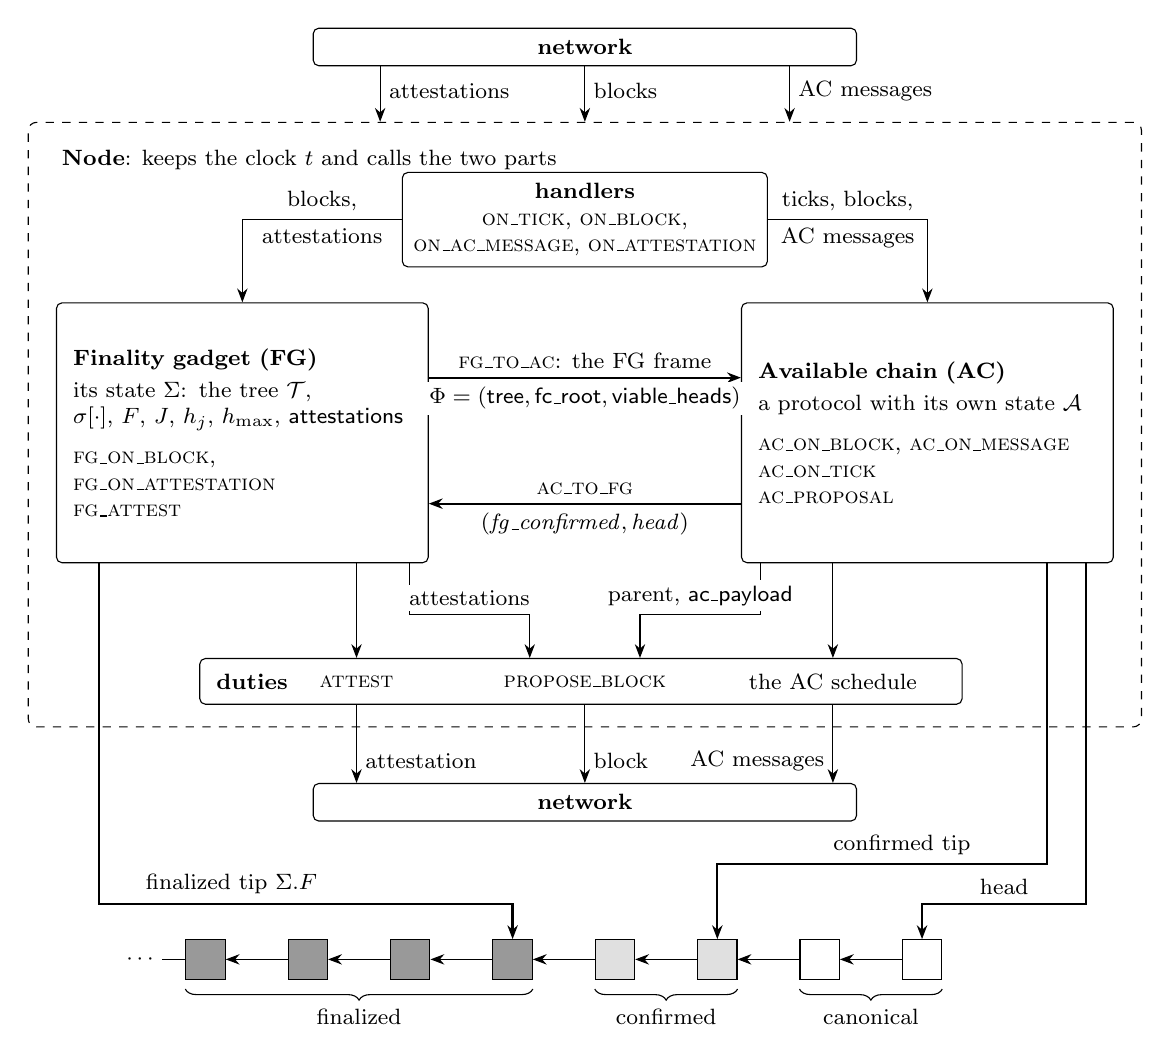
\begin{tikzpicture}[
  font=\footnotesize,
  >={Stealth[length=5pt]},
  part/.style={draw, rounded corners=2pt, align=left, inner sep=6pt,
    text width=4.3cm, minimum height=3.3cm, anchor=north west},
  small/.style={draw, rounded corners=2pt, align=center, inner sep=4pt},
  io/.style={align=center, inner sep=2pt},
  lab/.style={align=center, inner sep=2pt, fill=white},
]
% The two parts.
\node[part] (fg) at (0,0) {%
  \textbf{Finality gadget (FG)}\\[2pt]
  its state~$\Sigma$: the tree~$\T$,\\
  $\sigma[\cdot]$,\ $F$,\ $J$,\ $h_j$,\ $\hmax$, $\attestations$\\[5pt]
  $\fname{fg\_on\_block}$,\ $\fname{fg\_on\_attestation}$\\
  $\fname{fg\_attest}$};
\node[part] (ac) at (8.7,0) {%
  \textbf{Available chain (AC)}\\[2pt]
  a protocol with its own state~$\AC$\\[5pt]
  $\fname{ac\_on\_block}$,\ $\fname{ac\_on\_message}$\\
  $\fname{ac\_on\_tick}$\\
  $\fname{ac\_proposal}$};
% The interface.
\draw[->, thick] ($(fg.east)+(0,0.7)$) -- ($(ac.west)+(0,0.7)$)
  node[lab, midway, above=1pt] {$\fname{fg\_to\_ac}$: the FG frame}
  node[lab, midway, below=1pt] {$\Fr=(\tree,\fcroot,\allowed)$};
\draw[->, thick] ($(ac.west)+(0,-0.9)$) -- ($(fg.east)+(0,-0.9)$)
  node[lab, midway, above=1pt] {$\fname{ac\_to\_fg}$}
  node[lab, midway, below=1pt] {$(\mathit{fg\_confirmed},\mathit{head})$};
% Handlers.
\node[small] (hand)
  at ($(fg.north east)!0.5!(ac.north west)+(0,1.05)$)
  {\textbf{handlers}\\
   $\fname{on\_tick}$,\ $\fname{on\_block}$,\\
   $\fname{on\_ac\_message}$,\ $\fname{on\_attestation}$};
\draw[->] (hand.west) -| (fg.north)
  node[lab, pos=0.25, above=1pt] {blocks,}
  node[lab, pos=0.25, below=1pt] {attestations};
\draw[->] (hand.east) -| (ac.north)
  node[lab, pos=0.25, above=1pt] {ticks, blocks,}
  node[lab, pos=0.25, below=1pt] {AC messages};
% Duties: one box, narrower than the two parts.
\node[io] (att) at ($(fg.south)+(1.45,-1.5)$) {$\fname{attest}$};
\node[io] (prop) at ($(fg.south east)!0.5!(ac.south west)+(0,-1.5)$)
  {$\fname{propose\_block}$};
\node[io] (vote) at ($(ac.south)+(-1.2,-1.5)$) {the AC schedule};
\node[draw, rounded corners=2pt, inner sep=4pt,
  fit={($(fg.south |- att.north)+(-0.4,0)$)
       ($(ac.south |- att.south)+(0.3,0)$)}] (duties) {};
\node[anchor=west, inner sep=2pt] at ($(duties.west)+(4pt,0)$)
  {\textbf{duties}};
\draw[->] (att.north |- fg.south) -- (att.north |- duties.north);
\draw[->] ($(fg.south east)+(-0.25,0)$) -- ++(0,-0.65)
  -| ($(prop.north |- duties.north)+(-0.7,0)$)
  node[lab, pos=0.25, above=1pt] {attestations};
\draw[->] ($(ac.south west)+(0.25,0)$) -- ++(0,-0.65)
  -| ($(prop.north |- duties.north)+(0.7,0)$)
  node[lab, pos=0.25, above=1pt] {parent, $\acp$};
\draw[->] (vote.north |- ac.south) -- (vote.north |- duties.north);
% The node.
\node[anchor=south west, inner sep=2pt] (title)
  at ($(fg.north west)+(0,1.6)$)
  {\textbf{Node}: keeps the clock~$t$ and calls the two parts};
\node[draw, dashed, rounded corners=3pt, inner xsep=10pt, inner ysep=8pt,
  fit=(fg)(ac)(hand)(title)(duties)] (node) {};
% The network, above and below.
\node[small, minimum width=6.9cm] (netin)
  at ($(hand.north |- node.north)+(0,0.95)$) {\textbf{network}};
\foreach \dx/\txt in {-2.6/attestations, 0/blocks, 2.6/AC messages}
  \draw[->] ($(netin.south)+(\dx,0)$) -- ($(netin.south |- node.north)+(\dx,0)$)
    node[io, pos=0.45, right=1pt] {\txt};
\node[small, minimum width=6.9cm] (netout)
  at ($(prop.south |- node.south)+(0,-0.95)$) {\textbf{network}};
\draw[->] (att.south |- duties.south) -- (att.south |- netout.north)
  node[io, pos=0.72, right=1pt] {attestation};
\draw[->] (prop.south |- duties.south) -- (prop.south |- netout.north)
  node[io, pos=0.72, right=1pt] {block};
\draw[->] (vote.south |- duties.south) -- (vote.south |- netout.north)
  node[io, pos=0.72, left=1pt] {AC messages};
% The chain, with the outputs.
\coordinate (cy) at ($(fg.west |- netout.south)+(0,-1.75)$);
\foreach \i in {0,...,7}
  \node[draw, minimum size=0.5cm, inner sep=0pt] (b\i)
    at ($(cy)+(1.9+1.3*\i,0)$) {};
\foreach \i in {0,...,3}
  \node[draw, fill=black!40, minimum size=0.5cm, inner sep=0pt]
    at (b\i) {};
\foreach \i in {4,5}
  \node[draw, fill=black!12, minimum size=0.5cm, inner sep=0pt]
    at (b\i) {};
\node[io] at ($(b0.west)+(-0.55,0)$) {$\cdots$};
\draw (b0.west) -- ++(-0.3,0);
\foreach \i/\j in {0/1,1/2,2/3,3/4,4/5,5/6,6/7}
  \draw[<-] (b\i.east) -- (b\j.west);
\draw[decorate, decoration={brace, mirror, amplitude=4pt}]
  ($(b0.south west)+(0,-0.12)$) -- ($(b3.south east)+(0,-0.12)$)
  node[io, midway, below=5pt] {finalized};
\draw[decorate, decoration={brace, mirror, amplitude=4pt}]
  ($(b4.south west)+(0,-0.12)$) -- ($(b5.south east)+(0,-0.12)$)
  node[io, midway, below=5pt] {confirmed};
\draw[decorate, decoration={brace, mirror, amplitude=4pt}]
  ($(b6.south west)+(0,-0.12)$) -- ($(b7.south east)+(0,-0.12)$)
  node[io, midway, below=5pt] {canonical};
\draw[->, thick] ($(fg.south west)+(0.55,0)$) |- ($(b3.north)+(0,0.45)$)
  node[io, pos=0.66, above=1pt] {finalized tip $\Sigma.F$}
  -- (b3.north);
\draw[->, thick] ($(ac.south east)+(-0.85,0)$) |- ($(b5.north)+(0,0.95)$)
  node[io, pos=0.72, above=1pt] {confirmed tip}
  -- (b5.north);
\draw[->, thick] ($(ac.south east)+(-0.35,0)$) |- ($(b7.north)+(0,0.45)$)
  node[io, pos=0.75, above=1pt] {head}
  -- (b7.north);
\end{tikzpicture}
\captionof{figure}{The three parts.  The handlers feed each part from
the network, and the duties send to it.  The outputs point into one
chain: the finalized tip from the FG, and the confirmed tip and the head
from the AC.  Of the pair that $\fname{ac\_to\_fg}$ returns, the node
passes only $\mathit{fg\_confirmed}$ to the FG; the FG does not read the
head.}
\label{fig:system}
\end{center}

\paragraph{The name.}
Goldilocks is Goldfish with locks.  The name also says what the locks are
for.  Goldfish counts only the votes of one slot: it remembers too little
to keep a confirmed block when votes are missing.  A fork choice that
counts the latest vote of every validator, with no limit of age,
remembers too much.  A lock holds a confirmed block for about $k$~slots and
then expires: a memory that is neither too short nor too long.  The name
also fits the three tips of the chain.  The head is the newest, and it can
still change.  The finalized tip cannot change, but it comes late.  The
confirmed tip, the output of the available chain, is between the two: it
comes soon, and the locks protect it.

\paragraph{Pre-confirmations.}
A lock expires.  A PC does not.  At the confirmation update of slot~$s$,
at $t_s+6\Delta$, a node acks the raw result of the update when no lock
vetoes it, when it has at least $\mu=\lfloor n/2\rfloor+1$ clean early
supporters, and when the PC source of the slot-$s$ voters and the recent
PCs agree with it.  At least $\mu$ acks on one key form a PC.  A PC with
authority gives a second output, the \emph{strong} tip: the deepest common
ancestor of its target and the head.  The confirmed tip does not go below
the strong tip.  A PC with authority also moves the start of the walks of
the duties up to its target, and a lock that conflicts with the latest PC
has no effect.  The block for the FG is a supported prefix of a raw
result, not a PC.

\section{Composition}\label{sec:composition}

\subsection{Model}\label{sec:model}

A fixed set~$V$ of $n\geq1$ validators is given.  Every validator has
weight~$1$: for $S\subseteq V$, $w(S)=|S|$, and the quorum threshold is
$q=\lceil 2n/3\rceil$.  $\Delta$ is the delivery parameter of blocks and
AC messages, and $\Delta_F\geq\Delta$ is the delivery parameter of
attestations.  A bound is strict: the receiver processes the object at
a time strictly less than the deadline of the bound.  When the deadline is
a public time, the receiver thus processes the object before the tick at
that time.  Time is continuous, and the clock~$t$ of a node is the
current time.  The public times are the multiples of~$\Delta$.  A node
runs one tick at each public time.  A tick starts from the state as it
was before its public time, and each step of the tick reads the state
after the earlier steps of that tick.

A node is awake or asleep.  An asleep node receives nothing and runs no
tick, so it has no duty and no output.  An object that is sent while its
receiver sleeps, or that is not yet delivered when its receiver goes to
sleep, is delivered after the next wake: a delivery bound counts from the
later of the send time and that wake.  The node stamps an object with its
time of receipt.  A node that wakes restarts (Section~\ref{sec:store})
before it runs a tick or processes an object at that time; a crash is a
sleep.

The delivery bounds hold for every awake honest node.  An honest node
forwards an object when it accepts it: a block when the FG accepts it, an
AC message when the AC admits it, and an attestation when it passes the
checks.  This includes the objects that a block carries: a vote that the AC
admits from the payload of an accepted block, and an attestation of an
accepted block that enters the pool, are forwarded as wire objects of their
own, whether or not another node accepts the block.  So a delivery bound also counts from the time at which an honest
node first accepts the object; a receipt that is refused is not forwarded.  A node that runs
while its delivery is under the control of the adversary is faulty.

Slot~$s$ starts at the public time~$t_s$, with $t_0=0$ and
$t_s<t_{s+1}$, and has an assigned proposer.  The slot of a time~$t$, written $\slot(t)$, is
the greatest~$s$ with $t_s\leq t$.  Round~$r$ has the slots
$rR,\ldots,rR+R-1$, and $\round(s)=\lfloor s/R\rfloor$.  Its opening time
is $T_r=t_{rR}$.  Rounds are the heartbeat of the network for the
aggregation of attestations; no rule of the shared node reads them, and an
AC can use them.  The AC fixes the slot times and a lower bound on~$R$.

The local validator index is~$\valindex$.

\subsection{Blocks}\label{sec:blocks}

Every block~$B$ has a root~$B.\rootf$, slot~$B.\slot$, parent~$B.\parent$,
and proposer index~$B.\proposer$.  It has an AC payload~$B.\acp$ and a list
$B.\mathsf{attestations}$ of attestations (the FG payload).  The
order of each list and its repeated entries are part of the block.  The
block names its parent by root; the FG state must hold that parent in full,
with the same content, not only a block with the same root.  $B.\rootf$
is the fixed digest of
\[
 (B.\parent.\rootf,\ B.\slot,\ B.\mathsf{attestations},\ B.\acp).
\]
The AC fixes the encoding of its payload in this input.

The proposer signs a block with the slot key of $B.\proposer$.  A
validator signs an attestation with its fixed identity $\valindex\in V$.
A handler receives an object only when its signature is valid for its
signer and these checks pass: the signer of an attestation is in~$V$ and
its pairs have the forms of Section~\ref{sec:fg}; the slot key of
$B.\proposer$ signs a block~$B$; every attestation
that $B$ carries passes the same checks as on the wire;
$\Call{ac\_valid\_payload}{B}$ holds; an AC message passes the checks of
the AC; and $B.\rootf$ is the digest of the content of~$B$.  The check
drops an object that fails it, with no effect.

Processed blocks form a parent-closed tree rooted at~$\genesis$.  Write
$B\preceq C$ when $B=C$ or $B$ is an ancestor of~$C$, and write $B\prec C$
for strict ancestry.  Two blocks are compatible when one is an ancestor of
the other, and they conflict otherwise.  The depth of a block is the
number of parent edges from genesis.  ``Deepest'' means maximum depth;
ties use a fixed root order.

\subsection{State}\label{sec:store}

The node keeps the clock~$t$, the FG state~$\Sigma$ and the AC
state~$\AC$.  The FG state is
\[
 \Sigma=(\T,\sigma[\cdot],F,J,h_j,\hmax,\attestations).
\]
$\Sigma.\T$ is the tree of accepted blocks.  A block enters it only when
it extends~$\Sigma.F$, and no rule removes a block.
$\Sigma.\sigma[B]$ is the immutable chain state of an accepted
block.  $\Sigma.F$, $\Sigma.J$, $\Sigma.h_j$ and $\Sigma.\hmax$ are the
finality caches.  Section~\ref{sec:fg} defines the chain state and the
caches.  $\Sigma.\attestations$ holds
the processed attestations in full, one copy of each, in the order of
first acceptance, with no age limit and no limit per validator.  No rule
reads the time at which an attestation arrived; the pool serves inclusion
only.  Attestations reach the pool on the wire, through the node's own
$\Call{attest}{}$, and from the blocks that the FG accepts, after the
block's finality update.

Only the FG functions read and write~$\Sigma$, and only the AC functions
read and write~$\AC$.  The AC has no block store: the FG decides which
blocks are accepted, and the AC sees them through the FG frame.

The validator also keeps its anti-slashing record~$\Lambda$
(Section~\ref{sec:fg}).  The record belongs to the validator.  It is
durable: it persists through a restart.  A restart keeps~$\Lambda$,
$\Sigma$ and the clock, and it replaces~$\AC$ by
$\Call{ac\_restart}{\AC,\Fr,t}$, with $\Fr=\Call{fg\_to\_ac}{\Sigma}$
and $t$ the time of the restart.  The AC decides which part of its state
persists.

At initialization, $t=0$,
\[
 \Sigma.\T=\{\genesis\},\quad
 \Sigma.F=\Sigma.J=\genesis,\quad \Sigma.h_j=0,\quad \Sigma.\hmax=1,
\]
$\Sigma.\sigma[\genesis]$ is the initial chain state, the pool is empty,
and $\AC$ is the initial state of the AC.

\subsection{The FG frame}\label{sec:frame}

The FG frame is what the FG gives to the AC.  It is derived from the FG
state when used, and every call of one tick step reads the FG frame of the
same state:
\[
 \Fr=\Call{fg\_to\_ac}{\Sigma}=(\tree,\fcroot,\allowed).
\]
\begin{itemize}
\item $\Fr.\tree$ is the set of the accepted blocks that
  extend~$\Sigma.F$.  Write $\Fr.F$ for its root, the block~$\Sigma.F$.
\item $\Fr.\fcroot$ is a block of $\Fr.\tree$: the root of the fork
  choice.
\item $\Fr.\allowed$ is a set of blocks of $\Fr.\tree$ that
  extend~$\Fr.\fcroot$: the blocks on which a head walk may stop.
\end{itemize}
For a set $\mathit{tree}\subseteq\Fr.\tree$, the \emph{viable tree}
$\filtered(\Fr,\mathit{tree})$ is the set of the blocks of~$\mathit{tree}$
that extend~$\Fr.\fcroot$ and have a descendant in
$\mathit{tree}\cap\Fr.\allowed$.  It follows from the FG frame; it is not a
part of it.
$\Fr.F$ moves only to a descendant, also through a restart, because a
restart keeps~$\Sigma$.  So a block that leaves $\Fr.\tree$ does not
return.  Figure~\ref{alg:fg-store} computes the FG frame.

\subsection{The available chain}\label{sec:ac-interface}

An AC has a state~$\AC$, a set of wire messages, a block payload, and
these functions.  $t$ is the clock of the node.
\[
\begin{array}{l@{\qquad}l}
 \Call{ac\_valid\_payload}{B} & \text{stateless check of $B.\acp$},\\
 \Call{ac\_on\_message}{\AC,\Fr,t,m} & \text{an AC wire message arrives},\\
 \Call{ac\_on\_block}{\AC,\Fr,t,B} & \text{the FG accepted block $B$},\\
 \Call{ac\_on\_tick}{\AC,\Fr,t} & \text{the schedule of the AC; it can
   send AC messages},\\
 \Call{ac\_proposal}{\AC,\Fr,t} & \text{returns
   $(H,\mathit{ac\_payload})$: a parent and an AC payload, or $\bot$},\\
 \Call{ac\_to\_fg}{\AC,\Fr,t} & \text{returns
   $(\mathit{fg\_confirmed},\mathit{head})$; $\mathit{fg\_confirmed}=\bot$
   when no block is new},\\
 \Call{ac\_confirmed}{\AC,\Fr,t} & \text{returns the confirmed tip},\\
 \Call{ac\_head}{\AC,\Fr,t} & \text{returns the head},\\
 \Call{ac\_restart}{\AC,\Fr,t} & \text{returns the AC state after a restart}.
\end{array}
\]
The two receipt handlers $\Call{ac\_on\_message}{}$ and
$\Call{ac\_on\_block}{}$ can also send AC messages, as
$\Call{ac\_on\_tick}{}$ can.  These functions do not take the FG state.  The AC holds a block in its state only as
a name: the content of a block and its ancestry come from $\Fr.\tree$, or
from the block that a call supplies.  The AC must satisfy these
requirements.
\begin{enumerate}
\item Every head of a duty (the parent of a proposal, the head of a vote,
  the head that $\Call{ac\_to\_fg}{}$ returns) extends~$\Fr.\fcroot$.
  Such a head whose walk starts in $\filtered(\Fr,\mathit{tree})$ is in
  $\Fr.\allowed$.
\item A block $\mathit{fg\_confirmed}$ other than~$\bot$ is in
  $\filtered(\Fr,\Fr.\tree)$, and the returned head extends it.
\item The output of $\Call{ac\_head}{}$ extends~$\Fr.\fcroot$, and the
  confirmed tip extends~$\Fr.F$ and is an ancestor of that output.
\item The parent of a proposal is a head of the AC at that time.
\end{enumerate}

The protocol exposes three tips: the finalized tip~$\Sigma.F$, the
confirmed tip $\Call{ac\_confirmed}{\AC,\Fr,t}$ and the head
$\Call{ac\_head}{\AC,\Fr,t}$, with $\Fr=\Call{fg\_to\_ac}{\Sigma}$.  They
lie on one chain: the finalized tip is an ancestor of the confirmed tip,
and the confirmed tip is an ancestor of the head.

\subsection{Node}\label{sec:node}

The node runs the tick of a public time before it processes any object
received at that time.  It stamps an object with the time at which it
processes it, so an object received at a public time~$\tau$ counts as
received after the tick at~$\tau$.  A tick runs the schedule of the AC,
then the proposal duty at~$t_s$,
then the FG update.  A node processes its own block, its own AC
message and its own attestation at once.

The node drops a block of a future slot.  The FG then accepts the block
only when its full parent is held, no held block has its root, it
extends~$\Sigma.F$, and the assertions of its state transition hold.  A
failed test or assertion refuses the block before any write, and the AC
does not see a refused block.
No handler then runs for an object that it carries, and a later delivery
can call the handler again.  The proposer takes the parent and the AC
payload from the AC; when the AC returns~$\bot$, it makes no proposal.  It includes every attestation of its pool that is
valid against the state of the parent and is not already on the parent's
chain, in the order of its pool.

\emph{The FG update.}  After each tick the node asks the AC for an FG
update.  The AC returns a pair $(\mathit{fg\_confirmed},\mathit{head})$, with
$\mathit{fg\_confirmed}\neq\bot$ only when it has a new block to vouch
for.
$\mathit{fg\_confirmed}$ is the block up to which the AC vouches for the
chain of the head, for the FG.  The node gives the FG the block
$\mathit{fg\_confirmed}$ of each such pair, the \emph{source}, and the
client record decides whether an attestation follows: a target only as the
first vote at a height, and no entry twice (Section~\ref{sec:fg}).  The
height pair comes from the chain state of the source, and the finality
pair from the entry state of that chain state
(Section~\ref{sec:fg-client}).  The FG does not read the head.

The node functions take the input from outside the node: the time of a
tick, a received object, or the output of the AC for a duty.  They read
the clock~$t$ and pass $\Sigma$, $\AC$ and~$\Lambda$ to the two parts.

\captionof{figure}{Node: handlers and duties}\label{alg:node}
\nopagebreak
{\footnotesize
\begin{algorithmic}[1]
\Function{on\_tick}{$t$}
  \Comment{at each public time $t$}
  \State $s\gets\slot(t)$
  \State $\Fr\gets\Call{fg\_to\_ac}{\Sigma}$; \Call{ac\_on\_tick}{$\AC,\Fr,t$}
  \If{$s>0$ and $t=t_s$ and $\valindex$ is the slot-$s$ proposer}
    \State $P\gets\Call{ac\_proposal}{\AC,\Fr,t}$
    \Comment{$\bot$: the AC makes no proposal}
    \If{$P\neq\bot$} \State \Call{propose\_block}{$P$} \EndIf
  \EndIf
  \State $\Fr\gets\Call{fg\_to\_ac}{\Sigma}$;\quad
    $(\mathit{fg\_confirmed},\cdot)\gets\Call{ac\_to\_fg}{\AC,\Fr,t}$
  \Comment{$\bot$: no new block for the FG}
  \If{$\mathit{fg\_confirmed}\neq\bot$}
    \State \Call{attest}{$\mathit{fg\_confirmed}$}
    \Comment{the source; the FG does not read the head}
  \EndIf
\EndFunction
\vspace{1pt}
\Function{on\_block}{$B$}
  \If{$B.\slot>\slot(t)$} \State \Return \EndIf
  \If{not $\Call{fg\_on\_block}{\Sigma,B}$} \State \Return
    \Comment{the FG accepts or refuses the block}
  \EndIf
  \State $\Fr\gets\Call{fg\_to\_ac}{\Sigma}$; \Call{ac\_on\_block}{$\AC,\Fr,t,B$}
    \Comment{the frame after the FG accepted $B$}
\EndFunction
\vspace{1pt}
\Function{on\_ac\_message}{$m$}
  \State $\Fr\gets\Call{fg\_to\_ac}{\Sigma}$; \Call{ac\_on\_message}{$\AC,\Fr,t,m$}
\EndFunction
\vspace{1pt}
\Function{on\_attestation}{$a$}
  \State \Call{fg\_on\_attestation}{$\Sigma,a$}
\EndFunction
\vspace{1pt}
\Function{propose\_block}{$(H,\mathit{ac\_payload})$}
  \Comment{runs at $t_s$}
  \State $B\gets$ a block with $B.\parent=H$, $B.\slot=\slot(t)$,
    $B.\proposer=\valindex$, $B.\acp=\mathit{ac\_payload}$
  \State $B.\mathsf{attestations}\gets
    \Call{proposal\_attestations}{\Sigma,H}$
  \State broadcast $B$; \Call{on\_block}{$B$}
\EndFunction
\vspace{1pt}
\Function{attest}{$\mathit{fg\_confirmed}$}
  \State $a\gets\Call{fg\_attest}{\Sigma,\Lambda,\mathit{fg\_confirmed}}$
  \If{$a=\bot$} \State \Return \EndIf
  \State broadcast $a$; \Call{on\_attestation}{$a$}
\EndFunction
\end{algorithmic}
}


\section{Finality gadget}\label{sec:fg}

\subsection{Attestations and chain state}\label{sec:fg-state}

An attestation is
\[
 a=(\valindex,h,T,\tau,h_f,T_f).
\]
Its height pair $(h,T,\tau)$ is a vote at height $h\geq1$ that names the
block $T\neq\bot$ that brought the chain into height~$h$ on the
chain of $\mathit{fg\_confirmed}$: a \emph{target vote} when $\tau=\mathsf{false}$, and a
\emph{timeout} when $\tau=\mathsf{true}$.  Its finality pair $(h_f,T_f)$ is
empty, $(\bot,\bot)$, or has $T_f\neq\bot$ and $h_f<h$.
An attestation names $T$ and~$T_f$ by root, as a block names its parent.  A
test that compares $T$ or~$T_f$ with a block, or a pair with a pair of
$\sigma.\pendingFinality$, compares roots.

The chain state of an accepted block is
\[
 \begin{gathered}
 \Sigma.\sigma[B]=\Call{state\_transition}{\Sigma.\sigma[B.\parent],B},\\
 \sigma=(L,s,h,T_h,\targetParticipation,\progressBit,\pendingFinality,\finalityParticipation[\cdot],J,h_j,F,h_F).
 \end{gathered}
\]
$\sigma.L$ is the latest block, $\sigma.s=\sigma.L.\slot$, $\sigma.h$ is
the current height, and $\sigma.T_h$ is the block that brought the chain
into height~$\sigma.h$.  The arrays $\sigma.\targetParticipation$ and
$\sigma.\progressBit$ hold one Boolean value per validator.  Their quorum
sets are derived when used:
$\Qtarget(\sigma)=\{i:\sigma.\targetParticipation[i]\}$ and
$\Qprog(\sigma)=\{i:\sigma.\progressBit[i]\}$.  The pair
$(\sigma.J,\sigma.h_j)$ is the latest justification on the chain, and
$(\sigma.F,\sigma.h_F)$ is its latest finalization.  $\sigma.\pendingFinality$ is a list of at most $K_W$ pairs $(j,T)$ in
increasing order of~$j$, with $\sigma.h_F<j\leq\sigma.h_j$: the chain
justified~$T$ at height~$j$ and has not finalized it.  For each pair
$(j,T)$ of the list, the array $\sigma.\finalityParticipation[j]$ holds
one Boolean value per validator: whether a finality pair of that
validator names $(j,T)$ on the chain.  Its quorum set is
$\Qfin(\sigma,j)=\{i:\sigma.\finalityParticipation[j][i]\}$.  The
\emph{entry state} of~$\sigma$ is $\Sigma.\sigma[\sigma.T_h]$, the state
of the block that brought the chain into height~$\sigma.h$; its height
is~$\sigma.h$.  A justification ends its height, so every state with the
entry $(\sigma.h,\sigma.T_h)$ has the pair $(\sigma.J,\sigma.h_j)$ of its
entry state.  The height~$\sigma.h$ is \emph{bound} when $\sigma.h_j>0$
and $\sigma.h_j=\sigma.h-1$: the chain entered it by justifying its
predecessor $(\sigma.h_j,\sigma.J)$.  $K_W=2$, and
$\delta_{\mathrm{t}}\geq0$ is the timeout delay in slots; the AC sets its
value (Section~\ref{sec:sa-schedule}).  Initially
\[
 \sigma.L=\sigma.T_h=\sigma.J=\sigma.F=\genesis,\quad
 \sigma.s=0,\quad \sigma.h=1,\quad \sigma.h_j=\sigma.h_F=0,
\]
every array entry is false, and $\sigma.\pendingFinality$ is empty.

Every attestation that a block includes must be valid against the
parent's state: the attestation names the current entry of that state, or
it is a vote below the height of that state whose finality pair is a
pending pair of that state.

\subsection{Finality caches and frame}\label{sec:fg-frame}

$\Sigma.F$ is the accepted finalization, $(\Sigma.J,\Sigma.h_j)$ is the
lex-greatest justification of the accepted states that
extends~$\Sigma.F$, and $\Sigma.\hmax$ is the greatest accepted state
height.  With the tree, the chain states and the pool, these caches are the FG
state.  The FG frame is derived from it when used.

\emph{Frontier contest.}  The FG state is \emph{contested} when
$\Sigma.\hmax=\Sigma.h_j+1$ and some accepted block that
extends~$\Sigma.F$, with state height~$\Sigma.\hmax$, does not
extend~$\Sigma.J$.  The test reads the whole tree and the finality caches,
never the tree of a voter.  In a contest, the fork-choice root is~$\Sigma.F$ and the head height floor
is~$\Sigma.\hmax$.  Otherwise the fork-choice root is~$\Sigma.J$ when
$\Sigma.\hmax=\Sigma.h_j+1$ and $\Sigma.F$ when not, and the head height floor
is $\Sigma.\hmax-1$.  The head height floor gives the viable heads: the blocks
at or above the fork-choice root whose state height is at least the head height floor.
A block is \emph{viable} when its state height is at least the head height
floor.  Finality acceptance uses the same test: $\Sigma.F$ advances only to
a block with a viable descendant.

\captionof{figure}{FG: handlers, finality caches and frame}\label{alg:fg-store}
\nopagebreak
{\footnotesize
\begin{algorithmic}[1]
\Function{fg\_on\_block}{$\Sigma,B$}
  \Comment{returns whether $B$ is accepted}
  \If{$B.\rootf$ is the root of a block of $\Sigma.\T$ or
      $B.\parent\notin\Sigma.\T$ or $\Sigma.F\not\preceq B$}
    \State \Return $\mathsf{false}$
  \EndIf
  \State $\Sigma.\sigma[B]\gets
    \Call{state\_transition}{\Sigma.\sigma[B.\parent],B}$
  \Comment{a failed assertion: no write, return $\mathsf{false}$}
  \State add $B$ to $\Sigma.\T$
  \State \Call{update\_finality}{$\Sigma,\Sigma.\sigma[B]$}
  \ForAll{$a\in B.\mathsf{attestations}$}
    \State \Call{fg\_on\_attestation}{$\Sigma,a$}
  \EndFor
  \State \Return $\mathsf{true}$
\EndFunction
\vspace{1pt}
\Function{fg\_on\_attestation}{$\Sigma,a$}
  \State add $a$ to $\Sigma.\attestations$
  \Comment{one copy of each attestation}
\EndFunction
\vspace{1pt}
\Function{fg\_attest}{$\Sigma,\Lambda,\mathit{fg\_confirmed}$}
  \State $(h_c,T_c)\gets(\Sigma.\sigma[\mathit{fg\_confirmed}].h,
    \Sigma.\sigma[\mathit{fg\_confirmed}].T_h)$
  \State $\sigma_e\gets\Sigma.\sigma[T_c]$
  \Comment{the entry state: $\sigma_e.h=h_c$, $\sigma_e.T_h=T_c$}
  \State \Return $\Call{create\_attestation}{\Lambda,h_c,T_c,\sigma_e}$
  \Comment{an attestation or $\bot$}
\EndFunction
\vspace{1pt}
\Function{update\_finality}{$\Sigma,\sigma$}
  \State $\Sigma.\hmax\gets\max(\Sigma.\hmax,\sigma.h)$
  \If{$\Sigma.F\preceq\sigma.J$ \textbf{and}
      $(\sigma.h_j,\sigma.J.\rootf)>(\Sigma.h_j,\Sigma.J.\rootf)$}
    \Comment{lex order}
    \State $(\Sigma.J,\Sigma.h_j)\gets(\sigma.J,\sigma.h_j)$
  \EndIf
  \If{$\Sigma.F\prec\sigma.F$ \textbf{and} $\sigma.F\preceq\Sigma.J$
      \textbf{and} $\Call{has\_viable\_descendant}{\Sigma,\sigma.F}$}
    \State $\Sigma.F\gets\sigma.F$
  \EndIf
\EndFunction
\vspace{1pt}
\Function{fg\_contest}{$\Sigma$}
  \If{$\Sigma.\hmax\neq\Sigma.h_j+1$} \State \Return $\mathsf{false}$ \EndIf
  \State $\mathit{hmax\_blocks}\gets\{B\in\Sigma.\T:\Sigma.F\preceq B,\
    \Sigma.\sigma[B].h=\Sigma.\hmax\}$
  \Comment{the whole tree, never the tree of a voter}
  \State \Return $\exists B\in\mathit{hmax\_blocks},\ \Sigma.J\not\preceq B$
\EndFunction
\vspace{1pt}
\Function{head\_height\_floor}{$\Sigma$}
  \If{$\Call{fg\_contest}{\Sigma}$} \State \Return $\Sigma.\hmax$ \EndIf
  \State \Return $\Sigma.\hmax-1$
\EndFunction
\vspace{1pt}
\Function{get\_fc\_root}{$\Sigma$}
  \If{$\Sigma.\hmax=\Sigma.h_j+1$ \textbf{and not} $\Call{fg\_contest}{\Sigma}$}
    \State \Return $\Sigma.J$
  \EndIf
  \State \Return $\Sigma.F$
\EndFunction
\vspace{1pt}
\Function{is\_viable}{$\Sigma,B$}
  \State \Return $\Sigma.\sigma[B].h\geq\Call{head\_height\_floor}{\Sigma}$
\EndFunction
\vspace{1pt}
\Function{has\_viable\_descendant}{$\Sigma,B$}
  \State \Return $\exists B'\in\Sigma.\T,\ B\preceq B',\
    \Call{is\_viable}{\Sigma,B'}$
\EndFunction
\vspace{1pt}
\Function{fg\_to\_ac}{$\Sigma$}
  \State $\mathit{tree}\gets\{B\in\Sigma.\T:\Sigma.F\preceq B\}$
  \State $\mathit{fc\_root}\gets\Call{get\_fc\_root}{\Sigma}$
  \State $\mathit{viable\_heads}\gets\{B\in\mathit{tree}:
    \mathit{fc\_root}\preceq B,\ \Call{is\_viable}{\Sigma,B}\}$
  \State \Return $(\mathit{tree},\mathit{fc\_root},\mathit{viable\_heads})$
\EndFunction
\vspace{1pt}
\Function{proposal\_attestations}{$\Sigma,H$}
  \State \Return the $a\in\Sigma.\attestations$ with
    $\Call{valid\_attestation}{\Sigma.\sigma[H],a}$ that are not on $H$'s chain,
  \Statex \hspace{2em}in the order of the pool
\EndFunction
\end{algorithmic}
}

\subsection{Validator client}\label{sec:fg-client}

The anti-slashing record is
\[
 \Lambda=(\mathsf{target}[\cdot],\mathsf{timeout}[\cdot],
 \mathsf{lock}[\cdot],\mathsf{sent}):
\]
for each height~$h$, the first target that the validator sent at~$h$,
the set of the blocks that its timeouts at~$h$ name, and the target of
its first finality pair at~$h$, initially $(\bot,\emptyset,\bot)$; and
the set of the contents (height pair and finality pair) of the
attestations that it sent, initially empty.
$\Call{record\_attestation}{}$ is its only writer.  The tests read only
whether $\mathsf{timeout}[h]$ is empty, one block, or more, so a client
can store it as $\bot$, a root, or a mark for two or more blocks.  A
record that stores a Boolean at $\mathsf{timeout}[h]$, as an earlier
version of this client did, gives no root: false reads as the empty set,
and true reads as two or more blocks, never as a set within~$\{T\}$.

The client sends an attestation only with a height pair.  It sends a
target at a height only as its first vote at that height, and it names
each entry at most once at a height.  After a finality pair $(h,T)$ it
sends no row at~$h$, timeout or target vote, that names another block.
It reads the finality pair from the entry state of its source, not from
the head.  At a bound height the
pair is the predecessor $(h_j,J)$ when the record allows it, also when a
later state has finalized it, and empty otherwise.  At another height it
is the newest pending pair of the entry state that the record allows, or
empty.  So the pair is below the height of the height pair.

\captionof{figure}{FG: validator client}\label{alg:attn-full}
\nopagebreak
{\footnotesize
\begin{algorithmic}[1]
\Function{finality\_pair}{$\Lambda,\sigma_e$}
  \Comment{$\sigma_e$: the entry state of the source}
  \If{$\Call{bound}{\sigma_e}$}
    \Comment{the predecessor, even if a later state finalized it}
    \If{$\Call{permits}{\Lambda,\sigma_e.h_j,\sigma_e.J}$}
      \State \Return $(\sigma_e.h_j,\sigma_e.J)$
    \EndIf
    \State \Return $(\bot,\bot)$
  \EndIf
  \If{some $(j,T)\in\sigma_e.\pendingFinality$ has
      $\Call{permits}{\Lambda,j,T}$}
    \State \Return the one with the greatest~$j$
    \Comment{the newest permitted pair}
  \EndIf
  \State \Return $(\bot,\bot)$
\EndFunction
\vspace{1pt}
\Function{permits}{$\Lambda,j,T$}
  \Comment{the record allows the finality pair $(j,T)$}
  \State \Return $\Lambda.\mathsf{target}[j]\in\{\bot,T\}$ and
    $\Lambda.\mathsf{timeout}[j]\subseteq\{T\}$ and
    $\Lambda.\mathsf{lock}[j]\in\{\bot,T\}$
\EndFunction
\vspace{1pt}
\Function{height\_pair}{$\Lambda,h_c,T_c$}
  \If{$h_c=\bot$} \State \Return $(\bot,\bot,\bot)$ \EndIf
  \State $\mathit{lock}\gets\Lambda.\mathsf{lock}[h_c]$
  \If{$\mathit{lock}\notin\{\bot,T_c\}$}
    \State \Return $(\bot,\bot,\bot)$
    \Comment{locked elsewhere: wait out the height}
  \EndIf
  \If{$\Lambda.\mathsf{timeout}[h_c]\neq\emptyset$}
    \State \Return $(h_c,T_c,\mathsf{true})$
    \Comment{select a timeout for the current entry}
  \EndIf
  \If{$\Lambda.\mathsf{target}[h_c]\in\{\bot,T_c\}$}
    \State \Return $(h_c,T_c,\mathsf{false})$
    \Comment{vote for the target of that chain}
  \EndIf
  \State \Return $(h_c,T_c,\mathsf{true})$
  \Comment{otherwise time out at $h_c$}
\EndFunction
\vspace{1pt}
\Function{create\_attestation}{$\Lambda,h_c,T_c,\sigma_e$}
  \Comment{validator-client side: one chain state, no access to $\Sigma$}
  \State $(h_f,T_f)\gets\Call{finality\_pair}{\Lambda,\sigma_e}$
  \Comment{below $\sigma_e.h=h_c$}
  \State $(h,T,\tau)\gets\Call{height\_pair}{\Lambda,h_c,T_c}$
  \If{$h=\bot$} \State \Return $\bot$
    \Comment{no attestation without a height pair}
  \EndIf
  \If{some $b\in\Lambda.\mathsf{sent}$ has $b.h=h$ and ($\neg\tau$ or
      $b.T=T$)}
    \State \Return $\bot$
    \Comment{a target only as the first vote at $h$; no entry twice}
  \EndIf
  \State $a\gets(\valindex,h,T,\tau,h_f,T_f)$
  \State \Call{record\_attestation}{$\Lambda,a$}; \Return $a$
  \Comment{record, then send}
\EndFunction
\vspace{1pt}
\Function{record\_attestation}{$\Lambda,a$}
  \Comment{the only writer of $\Lambda$}
  \State add the content of $a$ to $\Lambda.\mathsf{sent}$
  \State $(h,T,\tau,h_f,T_f)\gets a$'s height and finality pairs
  \If{$T_f\neq\bot$} \State $\Lambda.\mathsf{lock}[h_f]\gets T_f$ \EndIf
  \If{$h\neq\bot$}
    \If{not $\tau$ and $\Lambda.\mathsf{target}[h]=\bot$}
      \State $\Lambda.\mathsf{target}[h]\gets T$
    \EndIf
    \If{$\tau$}
      \State $\Lambda.\mathsf{timeout}[h]\gets\Lambda.\mathsf{timeout}[h]\cup\{T\}$
    \EndIf
  \EndIf
\EndFunction
\end{algorithmic}
}

\captionof{figure}{FG: state transition}\label{alg:chain-full}
\nopagebreak
{\footnotesize
\begin{algorithmic}[1]
\Function{state\_transition}{$\sigma,B$}
  \State \textbf{assert} $B.\proposer=\operatorname{proposer}(B.\slot)$
  \State \textbf{assert} $B.\parent.\slot<B.\slot$
  \State \textbf{assert} every $a\in B.\mathsf{attestations}$ has
    $\Call{valid\_attestation}{\sigma,a}$
  \Comment{against the parent's state}
  \State $\sigma.s\gets B.\slot$
  \ForAll{$a\in B.\mathsf{attestations}$}
    \State $\sigma\gets\Call{process\_attestation}{\sigma,a}$
  \EndFor
  \State $\sigma.L\gets B$
  \State \Return $\Call{process\_height\_events}{\sigma}$
\EndFunction
\vspace{1pt}
\Function{valid\_attestation}{$\sigma,a$}
  \State $(h,T,\tau,h_f,T_f)\gets a$'s height and finality pairs
  \If{$(h,T)=(\sigma.h,\sigma.T_h)$}
    \State \Return $\mathsf{true}$
    \Comment{names the chain's own entry}
  \EndIf
  \State \Return $(h_f,T_f)\in\sigma.\pendingFinality$ and
    $h_f<h<\sigma.h$
  \Comment{an older vote with a useful finality pair}
\EndFunction
\vspace{1pt}
\Function{process\_attestation}{$\sigma,a$}
  \State $v\gets a.\valindex$;\quad
    $(h,T,\tau,h_f,T_f)\gets a$'s height and finality pairs
  \If{$(h_f,T_f)\in\sigma.\pendingFinality$}
    \State $\sigma.\finalityParticipation[h_f][v]\gets\mathsf{true}$
  \EndIf
  \If{$h=\sigma.h$ and $T=\sigma.T_h$}
    \Comment{names the chain's own entry}
    \State $\sigma.\progressBit[v]\gets\mathsf{true}$
    \If{not $\tau$}
      \State $\sigma.\targetParticipation[v]\gets\mathsf{true}$
    \EndIf
  \EndIf
  \State \Return $\sigma$
\EndFunction
\vspace{1pt}
\Function{process\_height\_events}{$\sigma$}
  \If{some $(j,T)\in\sigma.\pendingFinality$ has
      $w(\Qfin(\sigma,j))\geq q$}
    \State $(\sigma.F,\sigma.h_F)\gets(T,j)$ for the greatest such~$j$
  \EndIf
  \State remove from $\sigma.\pendingFinality$ every pair $(j,T)$ with
    $j\leq\sigma.h_F$
  \If{$w(\Qtarget(\sigma))\geq q$ \textbf{and}
      (not $\Call{bound}{\sigma}$ or $\sigma.h_F=\sigma.h_j$)}
    \Comment{a bound height waits for its predecessor}
    \State $(\sigma.J,\sigma.h_j)\gets(\sigma.T_h,\sigma.h)$
    \State append $(\sigma.h,\sigma.T_h)$ to $\sigma.\pendingFinality$;
      $\sigma.\finalityParticipation[\sigma.h]\gets\mathsf{false}^{V}$
    \State keep the newest $K_W$ pairs of $\sigma.\pendingFinality$
    \State \Return $\Call{advance\_height}{\sigma}$
  \EndIf
  \If{$w(\Qprog(\sigma))\geq q$ \textbf{and}
      $\sigma.s\geq\sigma.T_h.\slot+\delta_{\mathrm{t}}$}
    \Comment{timeouts count only after the delay}
    \State \Return $\Call{advance\_height}{\sigma}$
  \EndIf
  \State \Return $\sigma$
\EndFunction
\vspace{1pt}
\Function{advance\_height}{$\sigma$}
  \State $\sigma.h\gets\sigma.h+1$; \quad $\sigma.T_h\gets\sigma.L$
  \State $\sigma.\targetParticipation,
    \sigma.\progressBit\gets\mathsf{false}^{V}$
  \State \Return $\sigma$
\EndFunction
\vspace{1pt}
\Function{bound}{$\sigma$}
  \Comment{the chain entered $\sigma.h$ by justifying $\sigma.h-1$}
  \State \Return $\sigma.h_j>0$ and $\sigma.h_j=\sigma.h-1$
\EndFunction
\end{algorithmic}
}

\emph{Why a bound height waits for its predecessor.}  Faulty validators
can help to justify a height with target votes and withhold their
finality pairs.  Without the gate, the heights then advance before the
finality pairs of late honest validators arrive, and the window drops
each pair before it has a quorum.  With the gate, a justification at a
bound height~$h$ needs its predecessor $(\sigma.h_j,\sigma.J)$, with
$\sigma.h_j=h-1$, finalized in its block or before.  The gate reads
$\sigma.h_F$ after the finality step of the block, and the target bits
persist while the height is current, so a blocked target quorum
justifies in the first block that finalizes the predecessor, unless a
timeout has ended the height before.  While a bound height is current
and its predecessor is pending, the predecessor is the newest pair of the
window, and only an append, which ends the height, drops it; so a window
of one pair already keeps it, at every~$\Delta_F$.  A bound height that
cannot finalize its predecessor stays current until a block at least
$\delta_{\mathrm{t}}$ slots after its entry has a progress quorum, and
for ever when no such block comes.  That block crosses by timeout and
appends nothing: the predecessor stays pending at the crossing, and the
next height is unbound.  $K_W=2$ keeps the predecessor also through the next
append, the justification of that unbound height; a later append can
drop it.  A later finalization at a height of at least~$h-1$ covers it,
for example the finalization of that unbound justification at the bound
height that it enters.  The gate only withholds justifications: target
counting is unchanged, a justification still needs a target quorum and a
crossing a progress quorum, and the slashing conditions are unchanged.

\emph{Why the client reads the entry state.}  The pair $(h_j,J)$ is
the same in the source state and in its entry state, and the pending
pairs of the entry state are fixed by the entry.  So the finality pair
that a validator selects for an entry depends on its record, not on the
state of its source or of the head.  At a bound entry, the target votes
of the validators whose records allow the predecessor have the same
height pair and the same finality pair, also when a later state has
finalized the predecessor, so they aggregate.  The entry state of a bound
height has not finalized the predecessor, because the finality step of a
block precedes its append; the client carries the pair also when a later
state or the head has finalized it, so every row for the entry counts
toward the predecessor wherever it is still pending.  A validator whose
record does not allow the predecessor selects its height pair as before
and sends the empty finality pair: the predecessor does not turn its
target vote into a timeout.  At an unbound entry, records can select
different pending pairs, or none, so rows for one entry need not
aggregate.  A read of the head could give the pair of another height, or
none.  The pair is below the height of the height pair, so the client
needs no further test.

\subsection{Slashing conditions}\label{sec:fg-slashing}

Two attestations $a$ and~$b$ of one validator are \emph{slashable} when
one of two conditions holds.  The two attestations can be the same one.
\begin{description}
 \item[E1:] the finality pair of one is $(h,T)$, and the height pair of
   the other is at height~$h$ and names a block $T'\neq T$, as a timeout
   or as a target vote;
 \item[E2:] both height pairs are target votes at one height~$h$, for
   different blocks.
\end{description}
A timeout and a target vote at one height are not slashable, and two
timeouts at one height are not slashable.  A timeout $(h,T,\mathsf{true})$
and a finality pair $(h,T)$ are not slashable.  A validator is slashable in a
set of attestations when the set holds a slashable pair of that validator.
A validator that follows the client rules and keeps~$\Lambda$ sends no
slashable pair: it sends a target only as its first vote at a height, and
$\Call{finality\_pair}{}$ and $\Call{height\_pair}{}$ read the record
before they return a pair.

\captionof{figure}{FG: slashing conditions}\label{alg:fg-slashing}
\nopagebreak
{\footnotesize
\begin{algorithmic}[1]
\Function{e1}{$a,b$}
  \Comment{$a$'s finality pair against $b$'s height pair}
  \State $(h_f,T_f)\gets a$'s finality pair;\quad
    $(h',T',\tau')\gets b$'s height pair
  \State \Return $T_f\neq\bot$ and $h'=h_f$ and $T'\neq T_f$
\EndFunction
\vspace{1pt}
\Function{e2}{$a,b$}
  \Comment{two target votes at one height}
  \State $(h,T,\tau)\gets a$'s height pair;\quad
    $(h',T',\tau')\gets b$'s height pair
  \State \Return $h=h'$ and not $\tau$ and not $\tau'$ and $T\neq T'$
\EndFunction
\vspace{1pt}
\Function{slashable}{$a,b$}
  \If{$a.\valindex\neq b.\valindex$} \State \Return $\mathsf{false}$ \EndIf
  \State \Return $\Call{e1}{a,b}$ or $\Call{e1}{b,a}$ or $\Call{e2}{a,b}$
\EndFunction
\end{algorithmic}
}


\section{Available chain: PC-Goldilocks}\label{sec:sa}

The available chain of PC-Goldilocks is Goldfish with locks on confirmed
blocks and with PCs.  It reads the PC frame~$\Fr$ of the PC-SA node
(Section~\ref{sec:pc-node}), the clock and its own state~$\AC$.  The PC
frame is the FG frame with read-only access to the accepted blocks
of~$\Sigma.\T$ and to the refused roots.
Figure~\ref{fig:goldilocks} shows the protocol of
Figure~\ref{fig:system} with PC-Goldilocks in the place of the AC.
\begin{figure}[!ht]
\centering
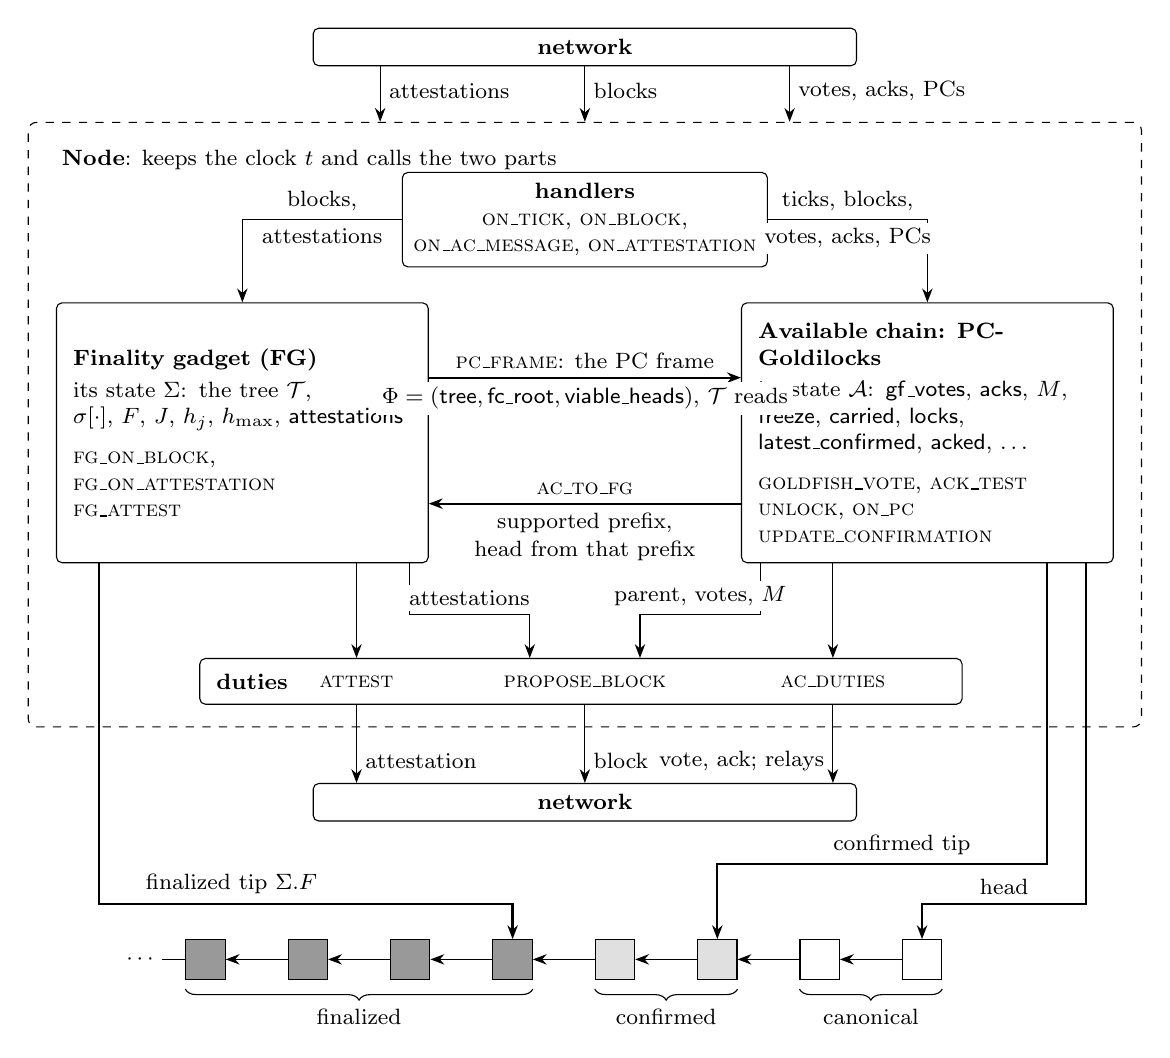
\begin{tikzpicture}[
  font=\footnotesize,
  >={Stealth[length=5pt]},
  part/.style={draw, rounded corners=2pt, align=left, inner sep=6pt,
    text width=4.3cm, minimum height=3.3cm, anchor=north west},
  small/.style={draw, rounded corners=2pt, align=center, inner sep=4pt},
  io/.style={align=center, inner sep=2pt},
  lab/.style={align=center, inner sep=2pt, fill=white},
]
% The two parts.
\node[part] (fg) at (0,0) {%
  \textbf{Finality gadget (FG)}\\[2pt]
  its state~$\Sigma$: the tree~$\T$,\\
  $\sigma[\cdot]$,\ $F$,\ $J$,\ $h_j$,\ $\hmax$, $\attestations$\\[5pt]
  $\fname{fg\_on\_block}$,\ $\fname{fg\_on\_attestation}$\\
  $\fname{fg\_attest}$};
\node[part] (ac) at (8.7,0) {%
  \textbf{Available chain: PC-Goldilocks}\\[2pt]
  its state~$\AC$: $\gfPool$, $\acks$, $M$,\\
  $\mathsf{freeze}$, $\mathsf{carried}$, $\locks$,\\
  $\latestConfirmed$, $\acked$, \ldots\\[5pt]
  $\fname{goldfish\_vote}$,\ $\fname{ack\_test}$\\
  $\fname{unlock}$,\ $\fname{on\_pc}$\\
  $\fname{update\_confirmation}$};
% The interface.
\draw[->, thick] ($(fg.east)+(0,0.7)$) -- ($(ac.west)+(0,0.7)$)
  node[lab, midway, above=1pt] {$\fname{pc\_frame}$: the PC frame}
  node[lab, midway, below=1pt] {$\Fr=(\tree,\fcroot,\allowed)$, $\T$ reads};
\draw[->, thick] ($(ac.west)+(0,-0.9)$) -- ($(fg.east)+(0,-0.9)$)
  node[lab, midway, above=1pt] {$\fname{ac\_to\_fg}$}
  node[lab, midway, below=1pt] {supported prefix,}
  node[lab, midway, below=11pt] {head from that prefix};
% Handlers.
\node[small] (hand)
  at ($(fg.north east)!0.5!(ac.north west)+(0,1.05)$)
  {\textbf{handlers}\\
   $\fname{on\_tick}$,\ $\fname{on\_block}$,\\
   $\fname{on\_ac\_message}$,\ $\fname{on\_attestation}$};
\draw[->] (hand.west) -| (fg.north)
  node[lab, pos=0.25, above=1pt] {blocks,}
  node[lab, pos=0.25, below=1pt] {attestations};
\draw[->] (hand.east) -| (ac.north)
  node[lab, pos=0.25, above=1pt] {ticks, blocks,}
  node[lab, pos=0.25, below=1pt] {votes, acks, PCs};
% Duties: one box, narrower than the two parts.
\node[io] (att) at ($(fg.south)+(1.45,-1.5)$) {$\fname{attest}$};
\node[io] (prop) at ($(fg.south east)!0.5!(ac.south west)+(0,-1.5)$)
  {$\fname{propose\_block}$};
\node[io] (vote) at ($(ac.south)+(-1.2,-1.5)$) {$\fname{ac\_duties}$};
\node[draw, rounded corners=2pt, inner sep=4pt,
  fit={($(fg.south |- att.north)+(-0.4,0)$)
       ($(ac.south |- att.south)+(0.3,0)$)}] (duties) {};
\node[anchor=west, inner sep=2pt] at ($(duties.west)+(4pt,0)$)
  {\textbf{duties}};
\draw[->] (att.north |- fg.south) -- (att.north |- duties.north);
\draw[->] ($(fg.south east)+(-0.25,0)$) -- ++(0,-0.65)
  -| ($(prop.north |- duties.north)+(-0.7,0)$)
  node[lab, pos=0.25, above=1pt] {attestations};
\draw[->] ($(ac.south west)+(0.25,0)$) -- ++(0,-0.65)
  -| ($(prop.north |- duties.north)+(0.7,0)$)
  node[lab, pos=0.25, above=1pt] {parent, votes, $M$};
\draw[->] (vote.north |- ac.south) -- (vote.north |- duties.north);
% The node.
\node[anchor=south west, inner sep=2pt] (title)
  at ($(fg.north west)+(0,1.6)$)
  {\textbf{Node}: keeps the clock~$t$ and calls the two parts};
\node[draw, dashed, rounded corners=3pt, inner xsep=10pt, inner ysep=8pt,
  fit=(fg)(ac)(hand)(title)(duties)] (node) {};
% The network, above and below.
\node[small, minimum width=6.9cm] (netin)
  at ($(hand.north |- node.north)+(0,0.95)$) {\textbf{network}};
\foreach \dx/\txt in {-2.6/attestations, 0/blocks, 2.6/{votes, acks, PCs}}
  \draw[->] ($(netin.south)+(\dx,0)$) -- ($(netin.south |- node.north)+(\dx,0)$)
    node[io, pos=0.45, right=1pt] {\txt};
\node[small, minimum width=6.9cm] (netout)
  at ($(prop.south |- node.south)+(0,-0.95)$) {\textbf{network}};
\draw[->] (att.south |- duties.south) -- (att.south |- netout.north)
  node[io, pos=0.72, right=1pt] {attestation};
\draw[->] (prop.south |- duties.south) -- (prop.south |- netout.north)
  node[io, pos=0.72, right=1pt] {block};
\draw[->] (vote.south |- duties.south) -- (vote.south |- netout.north)
  node[io, pos=0.72, left=1pt] {vote, ack; relays};
% The chain, with the outputs.
\coordinate (cy) at ($(fg.west |- netout.south)+(0,-1.75)$);
\foreach \i in {0,...,7}
  \node[draw, minimum size=0.5cm, inner sep=0pt] (b\i)
    at ($(cy)+(1.9+1.3*\i,0)$) {};
\foreach \i in {0,...,3}
  \node[draw, fill=black!40, minimum size=0.5cm, inner sep=0pt]
    at (b\i) {};
\foreach \i in {4,5}
  \node[draw, fill=black!12, minimum size=0.5cm, inner sep=0pt]
    at (b\i) {};
\node[io] at ($(b0.west)+(-0.55,0)$) {$\cdots$};
\draw (b0.west) -- ++(-0.3,0);
\foreach \i/\j in {0/1,1/2,2/3,3/4,4/5,5/6,6/7}
  \draw[<-] (b\i.east) -- (b\j.west);
\draw[decorate, decoration={brace, mirror, amplitude=4pt}]
  ($(b0.south west)+(0,-0.12)$) -- ($(b3.south east)+(0,-0.12)$)
  node[io, midway, below=5pt] {finalized};
\draw[decorate, decoration={brace, mirror, amplitude=4pt}]
  ($(b4.south west)+(0,-0.12)$) -- ($(b5.south east)+(0,-0.12)$)
  node[io, midway, below=5pt] {confirmed};
\draw[decorate, decoration={brace, mirror, amplitude=4pt}]
  ($(b6.south west)+(0,-0.12)$) -- ($(b7.south east)+(0,-0.12)$)
  node[io, midway, below=5pt] {canonical};
\draw[->, thick] ($(fg.south west)+(0.55,0)$) |- ($(b3.north)+(0,0.45)$)
  node[io, pos=0.66, above=1pt] {finalized tip $\Sigma.F$}
  -- (b3.north);
\draw[->, thick] ($(ac.south east)+(-0.85,0)$) |- ($(b5.north)+(0,0.95)$)
  node[io, pos=0.72, above=1pt] {confirmed tip}
  -- (b5.north);
\draw[->, thick] ($(ac.south east)+(-0.35,0)$) |- ($(b7.north)+(0,0.45)$)
  node[io, pos=0.75, above=1pt] {head}
  -- (b7.north);
\end{tikzpicture}
\caption{Figure~\ref{fig:system} with PC-Goldilocks as the available
chain.  The AC messages are Goldfish votes, acks and PCs.  The block
payload is the list of previous-slot votes with its support subset and
the latest PC maximum~$M$.  $\mathit{fg\_confirmed}$ is a supported prefix
of the raw result of the opening slot, and the head of the pair starts at
that prefix; the FG does not read that head.  The confirmed tip and the
strong tip are ancestors of the head (D17).}
\label{fig:goldilocks}
\end{figure}

\subsection{Schedule}\label{sec:sa-schedule}

Slot~$s$ starts at $t_s=4\Delta s$, so $\slot(t)=\lfloor t/(4\Delta)\rfloor$,
and it has the committee $\committee_s=V$.  Slot~$s$ has these public
actions:
\[
\begin{array}{c@{\qquad}l}
 t_s             & \text{proposal, for $s>0$; the carrier arm of slot $s$ opens},\\
 t_s+\Delta      & \text{Goldfish vote},\\
 t_s+2\Delta     & \text{confirmation freeze; early PC cut},\\
 t_s+3\Delta     & \text{vote freeze; PC freeze},\\
 t_s+5\Delta     & \text{unlocking against slot-$s$ votes},\\
 t_s+6\Delta     & \text{confirmation update of slot $s$; ack of slot $s$}.
\end{array}
\]
The last two actions of slot~$s$ occur in slot~$s+1$:
$t_s+5\Delta=t_{s+1}+\Delta$ is the vote time of slot~$s+1$, and
$t_s+6\Delta=t_{s+1}+2\Delta$ is its confirmation freeze.
Figure~\ref{fig:sa-timeline} shows the two slots.  The formula
$t_s=4\Delta s$ also gives the times of negative~$s$; the pools of a
negative slot are empty.  Write $v_s=t_s+\Delta$, $e_s=t_s+2\Delta$,
$z_s=t_s+3\Delta$, $q_s=t_s+5\Delta$ and $d_s=t_s+6\Delta$; so $q_s=v_{s+1}$
and $d_s=e_{s+1}$.

The parameters are these.
\begin{itemize}
\item $R\geq\lceil(6\Delta+\Delta_F)/(4\Delta)\rceil$ slots per round.  This
  is at least~$2$, because $\Delta_F\geq\Delta$.
\item The action time $a_r=T_r+6\Delta=d_{rR}$.  It is the time of the
  confirmation update of slot~$rR$.
\item The slow window of $k\geq2$ slots (S2 writes~$\ell$).  A lock that
  the confirmation update of slot~$s$ writes has the deadline
  $t_{s+k}+5\Delta=d_s+L$, with $L=(4k-1)\Delta$.
\item The absolute threshold $\mu=\lfloor n/2\rfloor+1$, a strict majority
  of the committee.  A PC needs $\mu$ acks, the ack test needs $\mu$ clean
  early supporters, and the unlocking and the opposition test count $\mu$
  opponents.  The fault bound is $a<\lceil n/2\rceil$, so $a<\mu$.
\item The FG window $K_W=2$ and the timeout delay
  $\delta_{\mathrm{t}}\geq e+c_F+k_F$ slots
  (Section~\ref{sec:fg-state}), with
  $c_F=\lceil(6\Delta+\Delta_F)/(4\Delta)\rceil$, the FG slack
  $k_F\geq0$, and the source exposure~$e$ of an entry
  (Section~\ref{sec:claims}, Loose BJ).  The candidate value
  $\delta_{\mathrm{t}}=R-1+c_F+k_F$ needs $e\leq R-1$, which is open.
\end{itemize}
The faulty set is static, in both roles.

\emph{The order at $d_s$.}  The tick at $d_s=e_{s+1}$ runs, in this order:
the confirmation update of slot~$s$ and its lock writes; the early PC cut
of slot~$s+1$; the ack test of slot~$s$; the preparation of the FG source
of slot~$s$.  Then the node selects all due outputs from that one state:
the ack of slot~$s$ and, when $d_s=a_r$, the FG action
(Section~\ref{sec:pc-node}).  No own object is processed between the
selection of the ack and the FG read.

\PCdiv{V1}{The ack of slot~$s$ is a new duty at $d_s$, on the raw result
of the confirmation update of slot~$s$.  The tick computes it, and the FG
row at $a_r$, from the same state after the update (S17, S29).  The early
PC cut at $e_s$ and the PC freeze at $z_s$ are new cuts at the existing
times of the confirmation freeze and the vote freeze.}

\PCdiv{V20}{The hidden seat bijection and the static faulty set are
model premises of PC-SA.  The threshold~$\mu$ is new: Goldilocks counts
``half of the committee or more'' for its fast test and unlocking.  For
odd~$n$ the two counts agree; for even~$n$, $\mu=n/2+1$ removes the tie at
$n/2$.}

\begin{figure}[!ht]
\centering
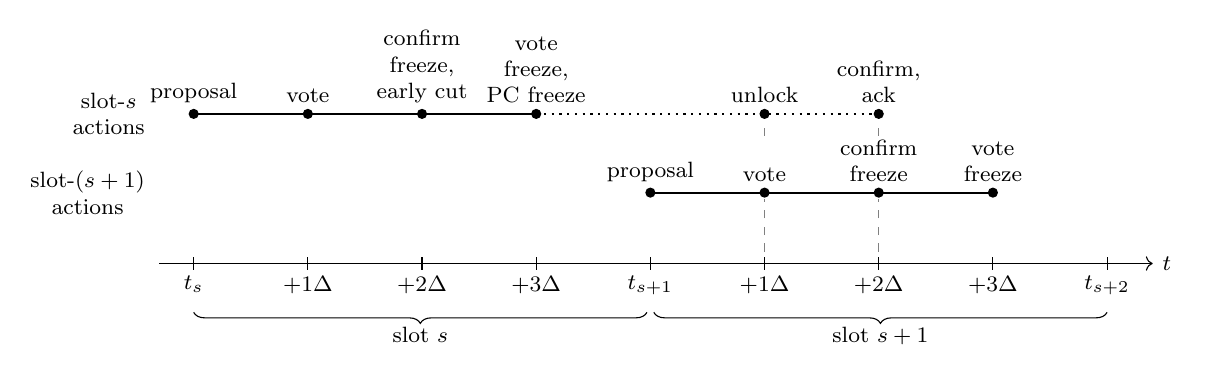
\begin{tikzpicture}[font=\footnotesize, x=1.45cm, y=1cm,
  ev/.style={circle, fill=black, inner sep=1.3pt},
  lab/.style={align=center, inner sep=1pt}]
% Time axis, t_s to t_{s+2}.
\draw[->] (-0.3,0) -- (8.4,0) node[right] {$t$};
\foreach \i in {0,...,8} \draw (\i,0.08) -- (\i,-0.08);
\node[lab, below] at (0,-0.12) {$t_s$};
\foreach \i in {1,2,3} \node[lab, below] at (\i,-0.12) {$+\i\Delta$};
\node[lab, below] at (4,-0.12) {$t_{s+1}$};
\foreach \i/\j in {5/1,6/2,7/3} \node[lab, below] at (\i,-0.12) {$+\j\Delta$};
\node[lab, below] at (8,-0.12) {$t_{s+2}$};
% Slot brackets.
\draw[decorate, decoration={brace, amplitude=4pt, mirror}]
  (0,-0.62) -- (3.97,-0.62) node[lab, midway, below=4pt] {slot $s$};
\draw[decorate, decoration={brace, amplitude=4pt, mirror}]
  (4.03,-0.62) -- (8,-0.62) node[lab, midway, below=4pt] {slot $s+1$};
% Actions of slot s.
\node[lab, anchor=east] at (-0.4,1.9) {slot-$s$\\actions};
\foreach \x/\txt in {0/proposal, 1/vote, 2/{confirm\\freeze,\\early cut}, 3/{vote\\freeze,\\PC freeze}, 5/unlock, 6/{confirm,\\ack}}
  { \node[ev] at (\x,1.9) {}; \node[lab, above] at (\x,2.0) {\txt}; }
\draw[thick] (0,1.9) -- (3,1.9);
\draw[thick, dotted] (3,1.9) -- (6,1.9);
% Actions of slot s+1.
\node[lab, anchor=east] at (-0.4,0.9) {slot-$(s+1)$\\actions};
\foreach \x/\txt in {4/proposal, 5/vote, 6/{confirm\\freeze}, 7/{vote\\freeze}}
  { \node[ev] at (\x,0.9) {}; \node[lab, above] at (\x,1.0) {\txt}; }
\draw[thick] (4,0.9) -- (7,0.9);
% The two coincidences.
\foreach \x in {5,6} { \draw[dashed, gray] (\x,0.15) -- (\x,0.82);
  \draw[dashed, gray] (\x,1.62) -- (\x,1.82); }
\end{tikzpicture}
\caption{The public actions of slots $s$ and~$s+1$.  The unlocking, the
confirmation update and the ack of slot~$s$ run in the ticks of the vote
and of the confirmation freeze of slot~$s+1$, before those actions
(Section~\ref{sec:sa-handlers}).}
\label{fig:sa-timeline}
\end{figure}

\subsection{State}\label{sec:sa-state}

\[
\begin{split}
 \AC=(&\gfPool[\cdot],\acks[\cdot],\timestamp[\cdot],
 \savedConfirmation[\cdot],\mathsf{gate\_ok}[\cdot],\mathsf{ft}[\cdot],
 \mathsf{ack\_ok}[\cdot],\locks,\latestConfirmed,\\
 &M,\mathsf{early},\mathsf{recent},\mathsf{unknown\_recent},
 \mathsf{interval},\mathsf{freeze}[2],\mathsf{carried}[2],\\
 &\mathsf{last\_freeze},\mathsf{fg\_candidate},\mathsf{sent\_keys},\acked[\cdot],\restartTime).
\end{split}
\]
Table~\ref{tab:sa-state} lists the fields.

\emph{PCs and roles.}  A PC is a certificate with a key
$(s,X,\delta)$: a slot, a block root and a signed depth
(Section~\ref{sec:sa-handlers}).  The AC keeps no set of PCs.  It keeps
\emph{roles}, and each role is a \emph{pair} $R=(R.\mathsf{latest},
R.\mathsf{held})$ of two PCs or~$\bot$.  $R.\mathsf{latest}$ is the
greatest-rank PC that entered the role.  $R.\mathsf{held}$ is a bounded
companion: a PC of the role whose target the node held when it entered,
with a rank at most that of $R.\mathsf{latest}$, and equal to it when the
target of $R.\mathsf{latest}$ is held.  The roles are~$M$, the two freeze
pairs and the two carrier pairs; $\mathsf{early}$ and the two PCs of
$\mathsf{recent}$ are single PCs.  These are the 13 PC records of
S2~\S4.9: $2+1+2+4+4$.

\begin{table}[!ht]
\centering
\footnotesize
\begin{tabular}{@{}>{\raggedright\arraybackslash}p{2.9cm}>{\raggedright\arraybackslash}p{3.4cm}>{\raggedright\arraybackslash}p{3.3cm}>{\raggedright\arraybackslash}p{2.7cm}>{\raggedright\arraybackslash}p{1.1cm}@{}}
\hline
Field & Holds & Written by & Read by & Restart\\
\hline
$\gfPool[s]$ & the accepted slot-$s$ votes, at most two distinct heads
  per validator, in the order of acceptance &
  \fname{on\_goldfish\_vote} & vote views, unlocking, confirmation,
  opposition & reset\\
$\acks[s]$ & the accepted slot-$s$ acks, at most two distinct
  $(X,\delta)$ per validator & \fname{on\_ack} & assembly & reset\\
$\timestamp[x]$ & the time at which the AC accepted the vote or the
  block~$x$; $\timestamp[\genesis]=-\infty$ &
  \fname{on\_goldfish\_vote}, \fname{ac\_on\_block} &
  resolution, voter block tree & reset\\
$\savedConfirmation[s]$, $\mathsf{gate\_ok}[s]$, $\mathsf{ft}[s]$ & the
  raw result of the slot-$s$ update, a block or~$\bot$, also when a lock
  vetoes it; whether no lock vetoed it; whether it has $\mu$ clean early
  supporters & \fname{update\_confirmation} & the slow test, the ack test,
  the source & reset\\
$\mathsf{ack\_ok}[s]$ & the result of the ack test of slot~$s$ &
  \fname{ac\_on\_tick} & \fname{ac\_duties} & reset\\
$\locks$ & the locks $(B,d)$: a block and a deadline, at most one per
  block & \fname{write\_lock}, \fname{unlock} & anchor, veto, unlocking &
  kept\\
$\latestConfirmed$ & the record of the confirmed tip &
  \fname{update\_confirmation} & \fname{ac\_confirmed} & kept\\
$M$ & the role pair of all processed PCs & \fname{on\_pc},
  \fname{target\_accepted} & authority, outputs, payload, B-HWC, freeze &
  kept\\
$\mathsf{early}$, $\mathsf{recent}$, $\mathsf{unknown\_recent}$,
  $\mathsf{interval}$ & the early cut $M.\mathsf{latest}$ at $e_w$, the
  summary of the PCs above it since $e_w$, and its slot~$w$ &
  \fname{early\_cut}, \fname{on\_pc} & B-HWC & reset\\
$\mathsf{freeze}[2]$, $\mathsf{last\_freeze}$ & two labelled pairs:
  $M$ at the PC freeze of a slot; the label of the last saved freeze &
  \fname{save\_freeze}, \fname{target\_accepted}, \fname{ac\_restart} & PC
  views, W, restart & kept\\
$\mathsf{carried}[2]$ & two labelled pairs: the PCs that the accepted
  blocks of a slot carry & \fname{open\_carrier}, \fname{on\_pc},
  \fname{target\_accepted} & PC views, W & rebuilt\\
$\mathsf{fg\_candidate}$ & the supported prefix of a slot, with its slot,
  or~$\bot$ & \fname{prepare\_fg\_source} & \fname{ac\_to\_fg} & reset\\
$\mathsf{sent\_keys}$ & the PC keys that the node relayed & \fname{on\_pc} &
  \fname{on\_pc} & kept\\
$\acked[s]$ & the block of the own ack of slot~$s$, or~$\bot$ &
  \fname{ac\_duties} & \fname{ack\_test} & kept\\
$\restartTime$ & the time of the latest restart & \fname{ac\_restart} &
  \fname{joined} & set\\
\hline
\end{tabular}
\caption{The fields of the PC-Goldilocks state.  The last column says what
a restart does to the field (Section~\ref{sec:sa-joining}).}
\label{tab:sa-state}
\end{table}

\emph{Target status.}  A role reads the target of its PC through the PC
frame.  A PC~$Q$ is \emph{active} when its target is a block of
$\Fr.\tree$; \emph{inert} when $Q=\bot$, or its target is held in
$\Sigma.\T$ but not in $\Fr.\tree$, or its target is refused; and
\emph{pending} otherwise.  The \emph{authority} of a role~$R$ is
$R.\mathsf{latest}$ when it is active, $R.\mathsf{held}$ when
$R.\mathsf{latest}$ is pending and $R.\mathsf{held}$ is active, and~$\bot$
otherwise (S14).  An inert latest gives no authority, and no lower PC takes
its place.  A frame move changes the status, never the rank.

\PCdiv{V4}{The PC roles are new state.  The AC keeps a fixed number of PC
records, not a set of held PCs, and it updates a role at the receipt of a
valid certificate, also when its target is missing (S18, S26).  The status
reads the frame at each use, as the liveness test of a lock does
(S14).}

\PCdiv{V7}{The gate flags, the ack flag, the early cut and its summary, the
source candidate, the sent keys and the own-ack record are new.  r5 keeps
the own-ack record in~$\Lambda$; here it is in~$\AC$, and a restart keeps
it (S21).  Goldilocks has $\AC.\fastConfirmed$; PC-Goldilocks has no such
field (V6).}

The other objects of the rules are derived when they are used, from the
current frame, the AC state and the time tests of their rules: a voter
block tree, a viable tree, a vote view, a score, a set of opponents, a
framed base, the anchor, the outputs and $\mathit{fg\_confirmed}$.

Initially the pools and the locks are empty, every role and PC record
is~$\bot$, and the freeze and carrier pairs have no label.  The saved
confirmation of every integer slot, also a negative one, is~$\bot$, every
flag is false, every own ack is~$\bot$, the record of the confirmed tip
is~$\genesis$, $\AC.\mathsf{last\_freeze}=-\infty$, and $\AC.\restartTime=t_0=0$
(S34).

\subsection{Messages and handlers}\label{sec:sa-handlers}

\emph{The vote.}  The wire message is the Goldfish vote, a tuple
$(\valindex,s,B)$ with $s\geq0$, from validator $\valindex\in\committee_s$
with head~$B$; it names its head by root.  The signer of a slot-$s$ vote
signs it with the slot-$s$ seat of~$\valindex$, under a bijection for each
slot between the seats and $\committee_s=V$.  For PC-SA the bijection is
hidden.  S2 and the Lean model call a Goldfish vote a \emph{HEAD}.

\emph{The ack.}  The second wire message is the \emph{ack}, a tuple
$(\valindex,s,X,\delta)$, from validator $\valindex\in\committee_s$: a
slot, a block root and a depth.  The signer signs all four fields with the
slot-$s$ seat of~$\valindex$, under the ack label, which is not the vote
label.  An honest node acks only its raw result~$X$ of slot~$s$, with the
depth $\delta=\depth(X)$ that it computes (Section~\ref{sec:sa-pc}).  An ack
counts only for exactly its key $(s,X,\delta)$.

\emph{The PC.}  The third wire message is the PC, a pair $P=(\kappa,A)$ of
a key $\kappa=(s,X,\delta)$ and an ordered list~$A$ of acks.  $P$ is
\emph{valid} when $A$ has at least $\mu$ acks from distinct validators and
each ack signs exactly~$\kappa$.  The check needs no block: it reads
neither the target, nor its slot, nor the frame.  Write $P.\slot=s$,
$P.\mathsf{target}=X$ and $P.\depth=\delta$.  The \emph{rank} of a PC is
$\rank(P)=(s,\delta,X)$, in lexicographic order, with the fixed root order
last.  A greater rank is preferred, and $\bot$ is below every PC.  Two PCs
with one key have the same rank; a role keeps the PC that it holds.  Every
valid PC has an honest signer, because $a<\mu$, so its signed depth is the
depth of its target, and a PC of slot~$s$ cannot exist before $d_s$.  A
later equivocation does not revoke a PC.

\PCdiv{V2}{The ack and the PC are new wire messages.  The ack signs the
depth of its target, so that the rank of a PC is known without its target
(S2~\S2.4).  A PC also arrives in a block (V3) and from local assembly
(V14).}

\emph{The payload.}  The payload of a block is
$B.\acp=(B.\mathsf{votes},B.\mathsf{support\_votes},B.\pc)$: a list of
slot-$(B.\slot-1)$ votes, a list whose entries occur in
$B.\mathsf{votes}$, and $B.\pc$, which is $\bot$ or a valid PC.  $B.\pc$
need not name an ancestor of~$B$, and its target can be missing at the
receiver.  The payload of~$\genesis$ is two empty lists and~$\bot$.  With
this payload the digest input of a block is
\[
 (B.\parent.\rootf,\ B.\slot,\ B.\mathsf{attestations},\
 B.\mathsf{votes},\ B.\mathsf{support\_votes},\ B.\pc).
\]
The digest commits to the full PC, with its key and its ack list.  The
support list records the proposer's view; it is not a second set of votes
to process.  A count reads distinct votes.

\emph{The payload check.}  $\Call{ac\_valid\_payload}{B}$ holds when every
vote in $B.\mathsf{votes}$ has slot $B.\slot-1$ and passes the stateless
checks of a wire vote, every entry of $B.\mathsf{support\_votes}$ occurs in
$B.\mathsf{votes}$, and $B.\pc$ is $\bot$ or a valid PC.  The check reads
neither the clock nor the pools nor the frame.  An AC message passes the
checks of the AC (Section~\ref{sec:blocks}) when it is a vote, an ack or a
PC that passes these stateless checks.

\PCdiv{V3}{The payload carries the latest maximum $M.\mathsf{latest}$ of
the proposer, also when it is inert or pending, so that the voters of the
slot read the same PC (S3).  The payload has no application value (S11):
S2 and the Lean model have one, but no rule of the AC reads it, and
Goldilocks has none.  A carried PC has no slot test: a valid certificate
is accepted with any target (S28, item~(u) of the Lean notes).}

\emph{Admission.}  $\Call{on\_goldfish\_vote}{}$ accepts a vote at time~$t$
when four conditions hold: its slot is $\slot(t)-1$ or $\slot(t)$, its
validator is in the committee of its slot, the pool does not hold it, and
the pool holds fewer than two distinct heads of its validator for that
slot.  An accepted vote enters the pool with the stamp~$t$, and the node
relays it.  $\Call{on\_ack}{}$ accepts an ack of any slot at most
$\slot(t)$, with no lower bound, when its validator is in the committee of
its slot, the pool does not hold its exact key from that validator, and
the pool holds fewer than two distinct $(X,\delta)$ of that validator for
that slot.  It reads no block.  The node relays an accepted ack, and then
it tries assembly on the key of the ack (Section~\ref{sec:sa-pc}).
$\Call{on\_pc}{}$ is the admission of a PC (Section~\ref{sec:sa-pc}).

\emph{Blocks.}  When the FG accepts a block~$B$, the node calls
$\Call{ac\_on\_block}{}$ with the frame after the FG step.  It stamps $B$
with the clock, gives each vote of $B.\mathsf{votes}$ to the admission
test, gives $B.\pc$ to $\Call{on\_pc}{}$ with the carrier slot $B.\slot$,
and then tells the roles that the target~$B$ arrived
($\Call{target\_accepted}{}$).

\emph{The tick.}  The tick runs the cuts of the PC roles at every awake
node, and the other steps only when the node is joined
(Section~\ref{sec:sa-joining}).  At $t_s$ it opens the carrier arm of
slot~$s$.  At $t_s+\Delta$, for $s>0$, a joined node unlocks against the
slot-$(s-1)$ votes.  At $t_s+2\Delta$, for $s>0$, a joined node runs the
confirmation update of slot~$s-1$; then every node makes the early PC cut
of slot~$s$; then a joined node runs the ack test of slot~$s-1$ and
prepares the FG source of slot~$s-1$.  At $t_s+3\Delta$ every node saves
the PC freeze of slot~$s$.  A tick runs before the objects of its time
(Section~\ref{sec:node}), so these steps read only objects with an earlier
stamp.  The vote, the ack, the proposal and the FG action are duties: the
PC-SA node selects them after the tick, from the state that the tick left
(Section~\ref{sec:pc-node}).  $\Call{ac\_duties}{}$ returns the vote and
the ack.

\PCdiv{V22}{The handlers also take the frame (S16), because the status of
a PC and the resolution of a vote read it.  The ack admission has no lower
slot bound, unlike the vote admission, because assembly reads old acks.
The ack admission has no slot test of the target (S2, \nm{Pools}).  The
handlers relay each accepted object (S20).  $\Call{ac\_on\_block}{}$ also
handles the carried PC and the target event.  The tick has the PC cuts,
the ack test and the source step, and the duties are selected after it
(S17).}

\captionof{figure}{PC-Goldilocks: tick and handlers}\label{alg:sa-interface}
\nopagebreak
{\footnotesize
\begin{algorithmic}[1]
\Function{ac\_on\_tick}{$\AC,\Fr,t$}
  \State $s\gets\slot(t)$;\quad $j\gets\Call{joined}{\AC,t}$
  \If{$t=t_s$} \State \Call{open\_carrier}{$\AC,s$} \EndIf
  \If{$t=t_s+\Delta$ and $s>0$ and $j$}
    \State \Call{unlock}{$\AC,\Fr,t,s-1$}
    \Comment{before the vote is selected}
  \EndIf
  \If{$t=t_s+2\Delta$}
    \If{$s>0$ and $j$}
      \State \Call{update\_confirmation}{$\AC,\Fr,t,s-1$}
      \Comment{reads the old early cut}
    \EndIf
    \State \Call{early\_cut}{$\AC,s$}
    \If{$s>0$ and $j$}
      \State $\AC.\mathsf{ack\_ok}[s-1]\gets\Call{ack\_test}{\AC,\Fr,s-1}$
      \State \Call{prepare\_fg\_source}{$\AC,\Fr,t,s-1$}
    \EndIf
  \EndIf
  \If{$t=t_s+3\Delta$} \State \Call{save\_freeze}{$\AC,s$} \EndIf
\EndFunction
\vspace{1pt}
\Function{ac\_duties}{$\AC,\Fr,t$}
  \Comment{PC: selected from the state after the tick (S17)}
  \State $s\gets\slot(t)$;\quad $\mathit{out}\gets[\,]$
  \If{not \Call{joined}{$\AC,t$} or $\valindex\notin\committee_s$}
    \State \Return $\mathit{out}$ \EndIf
  \If{$t=t_s+\Delta$}
    \State append $(\valindex,s,\Call{goldfish\_vote}{\AC,\Fr,t})$ to $\mathit{out}$
  \EndIf
  \If{$t=t_s+2\Delta$ and $s>0$ and $\AC.\mathsf{ack\_ok}[s-1]$}
    \State $X\gets\AC.\savedConfirmation[s-1]$;\quad $\AC.\acked[s-1]\gets X$
    \Comment{record, then send (D16)}
    \State append $(\valindex,s-1,X.\rootf,\depth(X))$ to $\mathit{out}$
  \EndIf
  \State \Return $\mathit{out}$
  \Comment{the node sends them; it admits them at delivery}
\EndFunction
\vspace{1pt}
\Function{ac\_on\_message}{$\AC,\Fr,t,m$}
  \Comment{PC: $\Fr$ is the receipt frame (S16)}
  \If{$m$ is a Goldfish vote}
    \Call{on\_goldfish\_vote}{$\AC,t,m$} \EndIf
  \If{$m$ is an ack} \Call{on\_ack}{$\AC,\Fr,t,m$} \EndIf
  \If{$m$ is a PC} \Call{on\_pc}{$\AC,\Fr,t,m,\bot$} \EndIf
\EndFunction
\vspace{1pt}
\Function{ac\_on\_block}{$\AC,\Fr,t,B$}
  \Comment{$\Fr$: the frame after the FG step (D18)}
  \If{$\AC.\timestamp[B]$ is not defined} \State $\AC.\timestamp[B]\gets t$ \EndIf
  \ForAll{$\mathit{vote}\in B.\mathsf{votes}$}
    \State \Call{on\_goldfish\_vote}{$\AC,t,\mathit{vote}$}
  \EndFor
  \If{$B.\pc\neq\bot$} \State \Call{on\_pc}{$\AC,\Fr,t,B.\pc,B.\slot$} \EndIf
  \State \Call{target\_accepted}{$\AC,B$}
  \Comment{the dependency arrived}
\EndFunction
\vspace{1pt}
\Function{on\_goldfish\_vote}{$\AC,t,\mathit{vote}$}
  \State $s\gets\slot(t)$
  \If{$\mathit{vote}.\slot<s-1$ or $\mathit{vote}.\slot>s$ or
    $\mathit{vote}.\valindex\notin\committee_{\mathit{vote}.\slot}$ or
    $\mathit{vote}\in\AC.\gfPool[\mathit{vote}.\slot]$}
    \State \Return \EndIf
  \If{$\AC.\gfPool[\mathit{vote}.\slot]$ holds two distinct votes by
    $\mathit{vote}.\valindex$}
    \State \Return \EndIf
  \State add $\mathit{vote}$ to $\AC.\gfPool[\mathit{vote}.\slot]$;
    $\AC.\timestamp[\mathit{vote}]\gets t$;\quad relay $\mathit{vote}$
\EndFunction
\vspace{1pt}
\Function{on\_ack}{$\AC,\Fr,t,\mathit{ack}$}
  \Comment{ingress: no join test}
  \State $(v,j,X,\delta)\gets\mathit{ack}$
  \If{$j>\slot(t)$ or $v\notin\committee_j$ or
    $\AC.\acks[j]$ holds $(v,j,X,\delta)$}
    \State \Return
    \Comment{no lower slot bound; no block read}
  \EndIf
  \If{$\AC.\acks[j]$ holds two distinct $(X',\delta')$ by $v$} \State \Return \EndIf
  \State add $\mathit{ack}$ to $\AC.\acks[j]$;\quad relay $\mathit{ack}$
  \State \Call{try\_assemble}{$\AC,\Fr,t,(j,X,\delta)$}
  \Comment{every new ack; no wait for the target (S26)}
\EndFunction
\end{algorithmic}
}

\subsection{Fork choice}\label{sec:sa-fc}

\emph{Resolution.}  A vote with head~$H$ is \emph{resolved} when
$\Sigma.\T$ holds a block with that root.  There is no test of $H.\slot$
against the slot of the vote (S41).  The test reads the accepted blocks of
the PC frame, not only $\Fr.\tree$.  The latest view and the merged view
of the vote keep a slot test of their own (Section~\ref{sec:sa-duties}).  The resolution time of a resolved vote is the later of its
stamp and the stamp of~$H$; a held block that the AC did not stamp in this
epoch has the stamp $\AC.\restartTime$.  The resolution time of any other
vote is~$+\infty$.

\PCdiv{V23}{Resolution, support, opposition and unlocking read the
cumulative tree $\Sigma.\T$ (S2~\S2.1).  Goldilocks reads $\Fr.\tree$.  A
vote whose head left $\Fr.\tree$ supports no block of $\Fr.\tree$ in both
forms; it can oppose a block of $\Fr.\tree$ only in PC-Goldilocks.  A frame
move thus cannot turn an ambiguous name into a resolved one.  Goldilocks
also requires $H.\slot$ to be at most the slot of the vote; PC-Goldilocks,
as the Lean, has no such test in resolution (S41).  A block of slot $w+1$
is accepted only from $t_{w+1}$, after the cut $t_w+2\Delta$ of the
confirmation update, of FT, of the source and of A2.  So the difference
reaches only the unlocking at $t_w+5\Delta$: a faulty slot-$w$ vote that
names an accepted block of slot $w+1$ can be an opponent there.  The latest
view and the merged view keep the slot test.}

\emph{Counting.}  In a set of votes, an \emph{equivocator} is a validator
with two distinct votes.  The \emph{supporters} of a block~$B$ are the
validators that are not equivocators and have a resolved vote in the
support set whose head extends~$B$.  The \emph{opponents} of~$B$ are the
validators that are not equivocators and have a resolved vote in the
support set whose head conflicts with~$B$.  The Goldfish score of~$B$ is
the number of its supporters plus the number of equivocators.  An
unresolved vote counts as a participant and can make an equivocator.

\emph{Vote views.}  A view is a pair of a vote set and its support subset.
$\Call{vote\_view}{}$ takes the slot-$s$ votes held before a cutoff, and as
support the members resolved before another cutoff.
$\Call{latest\_view}{}$ takes every held vote of the latest slot whose
votes are due: slot~$s-1$ before $t_s+2\Delta$, and slot~$s$ from then
on.  The head, the proposal and the head for the FG read the latest view.
The vote reads the merged view (Section~\ref{sec:sa-duties}).  A2 of the
ack test reads the gate view of the previous slot (Section~\ref{sec:sa-pc},
S32).

\emph{The walk.}  A walk starts at a block and descends through the
eligible children: at each step it takes the eligible child with the
greatest score, with ties by root order, and it stops when no child is
eligible.  A child is eligible when its parent is not a viable head, or it
holds a strict majority of the voters, or it is a block of the current
slot.  A walk starts at its start block also when that block is not in the
tree that it walks.

\emph{The framed base.}  Every walk of a duty starts from a role~$R$, a
view~$H$ and an age slot~$b$.  Let $Q$ be the authority of~$R$.  If
$Q=\bot$, the base is~$\Fr.\fcroot$.  Otherwise let $Y=\Call{anc}{}$ of $Q$:
the target of~$Q$ when $Q.\slot\geq b$, and else the deepest ancestor of
the target with fewer than $\mu$ opponents in~$H$ (the opposition release,
D21).  The base is the deepest block of the full viable tree
$U=\filtered(\Fr,\Fr.\tree)$ that is an ancestor of~$Y$, or
$\Fr.\fcroot$ when there is no such block.

\emph{The anchor.}  The anchor is the deepest effective locked block
(Section~\ref{sec:sa-locks}) of~$U$ that extends the base, or the base when
there is no such block.  The walk starts at the anchor and walks the viable
tree of its own domain.

\PCdiv{V10}{With no PC, the framed base is~$\Fr.\fcroot$ and the anchor
is the anchor of Goldilocks.  A PC with authority moves the start up to
the frame prefix of its target, so the walks of the duties stay above it
(r4 R8).  The opposition release projects the target down when $\mu$
current opponents oppose it (LATEST-ANC, D21); it never selects another
PC.  An inert or refused PC has no authority, and a pending PC uses the
held companion of its role (S14).  The locks above the base count from the
full viable tree, also for the vote.}

\emph{The head.}  $\Call{ac\_head}{}$ computes the head when it is read: at
slot~$0$ it is $\Fr.\fcroot$ (S23); otherwise a walk of the full viable
tree with the latest view, from the anchor of~$M$ with the age slot of
that view.  It reads the current frame, the current locks and the current
roles, so a change of~$\Fr$ moves it at once.  At~$t_s$ it is the parent
of the proposal.  The vote reads a frozen voter block tree, the merged view
and its own PC source, so its head can differ.  The head of the pair for
the FG starts at the source (D04), so it can also differ.

\emph{Why every duty head extends $\Fr.\fcroot$.}  The base extends
$\Fr.\fcroot$, the anchor extends the base, and a walk only descends.  A
walk that starts in the viable tree of a parent-closed domain ends on a
viable head, because a viable vertex that is not a viable head has an
eligible child toward its viable descendant (S2~\S2.6).

\emph{Why the head waits for no honest vote.}  When the delivery bounds
hold from $t_s+\Delta$ and the node is awake from $t_s+\Delta$, every honest
vote of slot~$s$ reaches it before $t_s+2\Delta$, the time from which the
head reads slot~$s$.

\captionof{figure}{PC-Goldilocks: fork choice}\label{alg:sa-fc}
\nopagebreak
{\footnotesize
\begin{algorithmic}[1]
\Function{resolution\_time}{$\AC,\Fr,\mathit{vote}$}
  \State $(v,s,H)\gets\mathit{vote}$
  \If{$H\notin\Fr.\T$}
    \Comment{PC: the cumulative tree; no slot test (V23, S41)}
    \State \Return $+\infty$
  \EndIf
  \State \Return $\max\{\AC.\timestamp[\mathit{vote}],\AC.\timestamp[H]\}$
  \Comment{an unstamped held block: $\AC.\restartTime$}
\EndFunction
\vspace{1pt}
\Function{equivocators}{$\mathit{votes}$}
  \State \Return $\{v:\mathit{votes}\text{ holds two distinct votes by }v\}$
\EndFunction
\vspace{1pt}
\Function{supporters}{$\mathit{votes},\mathit{support\_votes},s,B$}
  \State \Return $\{v\notin\Call{equivocators}{\mathit{votes}}:
    (v,s,B')\in\mathit{support\_votes}\text{ with }B\preceq B'\}$
\EndFunction
\vspace{1pt}
\Function{opponents}{$\mathit{votes},\mathit{support\_votes},s,B$}
  \Comment{PC: also for the opposition release}
  \State \Return $\{v\notin\Call{equivocators}{\mathit{votes}}:
    (v,s,B')\in\mathit{support\_votes}\text{ with $B'$ conflicting with }B\}$
\EndFunction
\vspace{1pt}
\Function{goldfish\_score}{$\mathit{votes},\mathit{support\_votes},s,B$}
  \State \Return $|\Call{equivocators}{\mathit{votes}}|+
    |\Call{supporters}{\mathit{votes},\mathit{support\_votes},s,B}|$
\EndFunction
\vspace{1pt}
\Function{vote\_view}{$\AC,\Fr,s,c_1,c_2$}
  \Comment{held before $c_1$; support resolved before $c_2$}
  \State $\mathit{votes}\gets\{\mathit{vote}\in\AC.\gfPool[s]:
    \AC.\timestamp[\mathit{vote}]<c_1\}$, in the order of the pool
  \State $\mathit{support\_votes}\gets\{\mathit{vote}\in\mathit{votes}:
    \Call{resolution\_time}{\AC,\Fr,\mathit{vote}}<c_2\}$
  \State \Return $(\mathit{votes},\mathit{support\_votes})$
\EndFunction
\vspace{1pt}
\Function{latest\_view}{$\AC,\Fr,t$}
  \State $s\gets\slot(t)$;\quad
    $s^*\gets s$ if $t\geq t_s+2\Delta$, else $s-1$
  \State $(\mathit{votes},\mathit{support\_votes})\gets
    \Call{vote\_view}{\AC,\Fr,s^*,+\infty,+\infty}$
  \State remove from $\mathit{support\_votes}$ each vote whose head has a
    slot above $s^*$
  \Comment{PC: \nm{outputBatch} (S41)}
  \State \Return $(\mathit{votes},\mathit{support\_votes},s^*)$
\EndFunction
\vspace{1pt}
\Function{ghost}{$\mathit{anchor},\mathit{tree},
  \mathit{score},\mathit{eligible}$}
  \State $H\gets\mathit{anchor}$
  \Loop
    \State $\mathit{children}\gets\{B:B\text{ is a child of }H\text{ in }
      \mathit{tree},\ \mathit{eligible}(B)\}$
    \If{$\mathit{children}=\emptyset$} \State \Return $H$ \EndIf
    \State $H\gets\arg\max_{B\in\mathit{children}}\mathit{score}(B)$,
      ties by root order
  \EndLoop
\EndFunction
\vspace{1pt}
\Function{goldfish\_eligible}{$\Fr,t,\mathit{votes},
  \mathit{support\_votes},s,B$}
  \If{$B.\parent\notin\Fr.\allowed$ or $B.\slot=\slot(t)$}
    \State \Return $\mathsf{true}$ \EndIf
  \State \Return $2\,\Call{goldfish\_score}{\mathit{votes},
    \mathit{support\_votes},s,B}>|\{v:\mathit{votes}\text{ holds a vote by }v\}|$
\EndFunction
\vspace{1pt}
\Function{viable\_tree}{$\Fr,\mathit{tree}$}
  \State \Return $\{B\in\mathit{tree}:\Fr.\fcroot\preceq B,\
    \exists W\in\mathit{tree}\cap\Fr.\allowed,\ B\preceq W\}$
\EndFunction
\vspace{1pt}
\Function{status}{$\Fr,Q$}
  \Comment{PC: three target states (S14)}
  \If{$Q=\bot$} \State \Return inert \EndIf
  \If{$Q.\mathsf{target}\in\Fr.\tree$} \State \Return active \EndIf
  \If{$Q.\mathsf{target}\in\Fr.\T$ or $\Fr.\mathsf{refused}(Q.\mathsf{target})$}
    \State \Return inert \EndIf
  \State \Return pending
\EndFunction
\vspace{1pt}
\Function{authority}{$\Fr,R$}
  \Comment{PC: $R=(R.\mathsf{latest},R.\mathsf{held})$}
  \State $Q\gets R.\mathsf{latest}$
  \If{$\Call{status}{\Fr,Q}=$ pending} \State $Q\gets R.\mathsf{held}$ \EndIf
  \State \Return $Q$ if $\Call{status}{\Fr,Q}=$ active, else $\bot$
\EndFunction
\vspace{1pt}
\Function{anc}{$Q,\mathit{votes},\mathit{support\_votes},b$}
  \Comment{PC: LATEST-ANC, the opposition release (D21)}
  \State $Y\gets Q.\mathsf{target}$
  \If{$Q.\slot\geq b$} \State \Return $Y$ \Comment{the age bypass} \EndIf
  \While{$|\Call{opponents}{\mathit{votes},\mathit{support\_votes},b,Y}|\geq\mu$}
    \State $Y\gets Y.\parent$
    \Comment{genesis has no opponents}
  \EndWhile
  \State \Return $Y$
\EndFunction
\vspace{1pt}
\Function{get\_anchor}{$\AC,\Fr,t,R,\mathit{votes},\mathit{support\_votes},b$}
  \State $U\gets\filtered(\Fr,\Fr.\tree)$;\quad $Q\gets\Call{authority}{\Fr,R}$
  \If{$Q=\bot$} \State $Y\gets\Fr.\fcroot$
  \Else
    \State $X\gets\Call{anc}{Q,\mathit{votes},\mathit{support\_votes},b}$
    \State $Y\gets$ the deepest $B\in U$ with $B\preceq X$, or $\Fr.\fcroot$
      if there is none
    \Comment{the framed base}
  \EndIf
  \State \Return the deepest $B\in U$ with $\Call{effective}{\AC,\Fr,t,B}$
    and $Y\preceq B$, or $Y$ if there is none
\EndFunction
\vspace{1pt}
\Function{get\_head}{$\AC,\Fr,t,\mathit{tree},
  \mathit{votes},\mathit{support\_votes},s,R,b$}
  \State $\mathit{anchor}\gets\Call{get\_anchor}{\AC,\Fr,t,R,\mathit{votes},
    \mathit{support\_votes},b}$
  \Comment{of the full viable tree}
  \State define $\mathit{score}(B)$ as
    $\Call{goldfish\_score}{\mathit{votes},\mathit{support\_votes},s,B}$
  \State define $\mathit{eligible}(B)$ as
    $\Call{goldfish\_eligible}{\Fr,t,\mathit{votes},
      \mathit{support\_votes},s,B}$
  \State \Return $\Call{ghost}{\mathit{anchor},\mathit{tree},
    \mathit{score},\mathit{eligible}}$
\EndFunction
\vspace{1pt}
\Function{ac\_head}{$\AC,\Fr,t$}
  \If{$\slot(t)=0$} \State \Return $\Fr.\fcroot$ \Comment{S23} \EndIf
  \State $(\mathit{votes},\mathit{support\_votes},s^*)\gets
    \Call{latest\_view}{\AC,\Fr,t}$
  \State \Return $\Call{get\_head}{\AC,\Fr,t,\filtered(\Fr,\Fr.\tree),
    \mathit{votes},\mathit{support\_votes},s^*,\AC.M,s^*}$
\EndFunction
\end{algorithmic}
}

\subsection{Locks}\label{sec:sa-locks}

\emph{Locks.}  $\AC.\locks$ is a set of locks $(B,d)$, a block and a
deadline, at most one per block.  A lock is \emph{live} when $d>t$ and
$B\in\Fr.\tree$.  A lock is \emph{effective} when it is live and the
target of $M.\mathsf{latest}$ does not conflict with~$B$; an unknown target
conflicts with nothing, so it keeps the lock.  A block is \emph{locked} when
it is the block of an effective lock.  This lock is not the finality lock
$\Lambda.\mathsf{lock}[h]$ of the record.

\emph{Effects.}  An effective lock has two effects.  It can be the anchor
of a walk (Section~\ref{sec:sa-fc}), and it vetoes a confirmation result
that conflicts with it (Section~\ref{sec:sa-confirmation}).  A PC changes
no lock: a lock that conflicts with the target of $M.\mathsf{latest}$ is
not effective while that PC is the maximum, and it is effective again
when a higher compatible PC replaces it.

\emph{Deadlines.}  A write on a block that already has a lock keeps the
later of the two deadlines, so no step moves a deadline back.  A lock is
not live from its deadline on.  A lock that is not live changes no
decision; a restart can keep it.

\emph{Unlocking.}  At $t_s+5\Delta$, unlocking removes each stored lock
$(B,d)$ with $d>t$ for which $\mu$ or more validators are non-equivocating
opponents: validators with a slot-$s$ vote received and resolved before
$t_s+5\Delta$ whose head conflicts with~$B$.  It inspects every stored
unexpired lock, also one that is not effective.  It keeps the deadline of
every other lock.

\emph{Why unlocking is well defined.}  The opponents of an ancestor are a
subset of the opponents of a descendant, so the locks on one chain that
survive are on a prefix of that chain.  A lock on~$\Fr.F$ or below it has
no effect: it vetoes no result, because every result extends~$\Fr.F$, and
it is never the anchor.  No rule acts on the locks when $\Fr.F$ advances.

\PCdiv{V5}{Goldilocks keeps at most one lock per deadline, a block is
locked when it is an ancestor of the block of a live lock, and unlocking
moves a lock back to the deepest block with fewer opponents than half of
the committee.  PC-Goldilocks keeps one lock per block and writes a lock
on each block of the path that it locks, so for the same writes the two
forms lock the same blocks.  Unlocking removes a lock with $\mu$
opponents and does not move it back.  A lock has no rank.  The PC test of
the old text (L*$'$) is replaced by the M-veto: a lock that conflicts with
$M.\mathsf{latest}$ is not effective (S13, S30).}

\captionof{figure}{PC-Goldilocks: locks}\label{alg:sa-unlock}
\nopagebreak
{\footnotesize
\begin{algorithmic}[1]
\Function{effective}{$\AC,\Fr,t,B$}
  \State \Return $\AC.\locks$ holds $(B,d)$ with $d>t$, $B\in\Fr.\tree$, and
  \Statex \hspace{2em}$\Call{lock\_compatible}{\Fr,\AC.M.\mathsf{latest},B}$
  \Comment{PC: the M-veto (S30)}
\EndFunction
\vspace{1pt}
\Function{unlock}{$\AC,\Fr,t,s$}
  \Comment{at $t_s+5\Delta$, against the slot-$s$ votes}
  \State $(\mathit{votes},\mathit{support\_votes})\gets
    \Call{vote\_view}{\AC,\Fr,s,t,t}$
  \Comment{every stamp is below $t_s+5\Delta$}
  \ForAll{$(B,d)\in\AC.\locks$ with $d>t$}
    \Comment{PC: every stored unexpired lock}
    \If{$|\Call{opponents}{\mathit{votes},\mathit{support\_votes},s,B}|\geq\mu$}
      \State remove $(B,d)$ from $\AC.\locks$
      \Comment{PC: remove; no move back}
    \EndIf
  \EndFor
\EndFunction
\vspace{1pt}
\Function{write\_lock}{$\AC,B,d$}
  \Comment{PC: one lock per block}
  \If{$\AC.\locks$ holds a lock $(B,d')$}
    \State replace it by $(B,\max\{d',d\})$
  \Else
    \State add $(B,d)$ to $\AC.\locks$
  \EndIf
\EndFunction
\end{algorithmic}
}

\subsection{Confirmation}\label{sec:sa-confirmation}

At $t_s+6\Delta$ the AC evaluates slot~$s$ once.  The update runs in the
tick at $t_s+6\Delta$, before the objects of that time, so every vote and
block that it reads has an earlier stamp.  Only a joined node runs it; the
saved result of a node that is not joined stays~$\bot$.

\emph{The result.}  The walk of the update starts at~$\Fr.F$ and descends
in $\Fr.\tree$ through the children that hold a strict majority of the
participants of the slot.  Support counts only the votes resolved before
$t_s+2\Delta$, the confirmation freeze, of validators with no second vote, and
the participants are the validators with a vote.  The result is the end of
the walk when that block holds the majority, $\Fr.F$ included, and $\bot$
otherwise.  The walk has no current-slot exception and no viable-head
exception.

\emph{The saved result, the flags and the veto.}  The update saves the
result in $\AC.\savedConfirmation[s]$, also when a lock vetoes it, for the
slow test of later slots and for the ack.  It sets $\AC.\mathsf{ft}[s]$
when the result has at least $\mu$ supporters.  An effective lock that
conflicts with the result vetoes it, and $\AC.\mathsf{gate\_ok}[s]$
records that no lock vetoed it.  An update with no result or with a vetoed
result stops there.

\emph{The record.}  Otherwise the update advances the record
$\AC.\latestConfirmed$ by the $\Call{advance}{}$ rule: an ancestor of the
record leaves it unchanged, and an extension or a conflicting block
replaces it.  No voting rule reads the record.

\emph{The lock.}  Then the update writes a lock with the deadline
$t_{s+k}+5\Delta$ on each non-genesis block~$B$ of the result's chain that
passes two tests.  The slow test: the saved results of slot~$s$ and of
the previous $k-1$ slots are all blocks that extend~$B$.  The history test
(B-HWC): $B$ is compatible with the targets of $M.\mathsf{latest}$ and of
the early cut $\AC.\mathsf{early}$, and with every PC that the summary
$\AC.\mathsf{recent}$ holds, and no PC with an unknown target entered the
summary.  A PC whose target is not held fails the test: an unknown history
grants no new write.  Each test holds for the ancestors of a block that
passes it, so the update locks a prefix of the path.

\emph{Why the history test.}  The test is the MC-HWC rule of r4: a write
on~$B$ is permitted only if each PC accepted before $t_s+6\Delta$ that
conflicts with~$B$ has a greater, compatible PC accepted before
$t_s+2\Delta$.  The early cut keeps the maximum at $t_s+2\Delta$, and the
summary keeps every constraint of the PCs above it that arrived in
$[t_s+2\Delta,t_s+6\Delta)$ with two PCs and one block (S2~\S4.6--4.7).

\PCdiv{V9}{Goldilocks writes one lock, on the deepest block that passes
the fast test or the slow test.  PC-Goldilocks has no fast test (V6), it
adds the history test, and it writes a lock on each block of the path
(V5).  The history test keeps the update from writing a lock across a PC
that the next voters can read.  Two smaller changes follow S2 and the
Lean (Gate:22--23, Walks:56--62): the path is taken in $\Sigma.\T$, not in
$\Fr.\tree$, and the slow test does not require each saved result to be in
$\Fr.\tree$.  For a block $B\in\Fr.\tree$ the two forms agree: a saved
result that extends~$B$ extends $\Fr.F$, so it is in $\Fr.\tree$.  A block
of the path below $\Fr.F$ can get a lock here and not in Goldilocks; that
lock is never effective, because an effective lock is in $\Fr.\tree$.
The slow test here includes slot~$s$ itself; in Goldilocks slot~$s$
passes because $B\preceq C$.}

\PCdiv{V6}{Goldilocks saves in $\AC.\fastConfirmed$ the blocks that pass
the fast test, for the block for the FG.  PC-Goldilocks has no fast test
and no such set: the PC takes the place of the fast lock, and the block
for the FG is a supported prefix (Section~\ref{sec:sa-duties}).}

\emph{The outputs.}  At each awake output read, the AC uses the current
frame and does not change its state.  Let $H=\Call{ac\_head}{}$, let $Q$ be
the authority of~$M$, $P=Q.\mathsf{target}$ when $Q\neq\bot$ and
$P=\Fr.F$ otherwise, $S$ the record when it extends~$\Fr.F$ and $\Fr.F$
otherwise, and $C=S$ when $P\preceq S$ and $C=P$ otherwise.  Then
\[
 \mathit{strong}=\operatorname{dca}(P,H),\qquad
 \mathit{confirmed}=\mathit{stable}=\operatorname{dca}(C,H),
\]
where dca is the deepest common ancestor.  $\Call{ac\_confirmed}{}$ and the
stable output return the confirmed tip, $\Call{ac\_strong}{}$ returns the
strong tip, and the finalized output is~$\Fr.F$.  Both $P$ and $S$ extend
$\Fr.F$, $P\preceq C$, and $\Fr.F\preceq\Fr.\fcroot\preceq H$, so
\[
 \Fr.F\preceq\mathit{strong}\preceq\mathit{confirmed}=\mathit{stable}\preceq H
\]
at every awake read, also across a wake (S2~\S2.7).

\PCdiv{V17}{Goldilocks returns the deepest common ancestor of its record
and the head.  PC-Goldilocks does the same with the PC floor~$C$, and it
has the strong tip as a second output (D17).  Both are ancestors of the
head, so requirement~3 of Section~\ref{sec:ac-interface} holds.  The old
text returned the PC floor without the clamp; that floor kept the target
of a stranded PC, and the clamp can drop below it (R7 Section~4.4).}

\captionof{figure}{PC-Goldilocks: confirmation}\label{alg:sa-gate}
\nopagebreak
{\footnotesize
\begin{algorithmic}[1]
\Function{get\_confirmation}{$\AC,\Fr,s$}
  \Comment{at $t_s+6\Delta$; every stamp is below it}
  \State $(\mathit{votes},\mathit{early})\gets
    \Call{vote\_view}{\AC,\Fr,s,+\infty,t_s+2\Delta}$
  \Comment{the whole pool decides who equivocates}
  \State define $\mathit{score}(B)$ as
    $|\Call{supporters}{\mathit{votes},\mathit{early},s,B}|$
  \State define $\mathit{eligible}(B)$ as
    $2\,\mathit{score}(B)>|\{v:\mathit{votes}\text{ holds a vote by }v\}|$
  \State $H\gets\Call{ghost}{\Fr.F,\Fr.\tree,\mathit{score},
    \mathit{eligible}}$
  \State \Return $(H,\mathit{score}(H))$ if $\mathit{eligible}(H)$, else
    $(\bot,0)$
\EndFunction
\vspace{1pt}
\Function{update\_confirmation}{$\AC,\Fr,t,s$}
  \Comment{at $t_s+6\Delta$, joined; before the early cut of slot $s+1$}
  \State $(C,p)\gets\Call{get\_confirmation}{\AC,\Fr,s}$
  \State $\AC.\savedConfirmation[s]\gets C$;\quad
    $\AC.\mathsf{ft}[s]\gets(C\neq\bot\text{ and }p\geq\mu)$
  \State $\AC.\mathsf{gate\_ok}[s]\gets(C\neq\bot$ and no
    $B$ with $\Call{effective}{\AC,\Fr,t,B}$ conflicts with $C)$
  \If{not $\AC.\mathsf{gate\_ok}[s]$} \State \Return \EndIf
  \State $\AC.\latestConfirmed\gets
    \Call{advance}{\Fr,\AC.\latestConfirmed,C}$
  \ForAll{$B\in\Fr.\T$ with $B\neq\genesis$, $B\preceq C$}
    \If{every $j$ with $s-k<j\leq s$ has $\AC.\savedConfirmation[j]\neq\bot$
      and $B\preceq\AC.\savedConfirmation[j]$}
      \Comment{the slow test}
      \If{\Call{history\_ok}{$\AC,\Fr,B$}}
        \Comment{PC: B-HWC}
        \State \Call{write\_lock}{$\AC,B,t_{s+k}+5\Delta$}
      \EndIf
    \EndIf
  \EndFor
\EndFunction
\vspace{1pt}
\Function{history\_ok}{$\AC,\Fr,B$}
  \Comment{PC: unknown geometry grants no write}
  \State \Return $\Call{known\_compatible}{\Fr,\AC.M.\mathsf{latest},B}$ and
    $\Call{known\_compatible}{\Fr,\AC.\mathsf{early},B}$
  \Statex \hspace{2em}and not $\AC.\mathsf{unknown\_recent}$ and
    $\Call{recent\_compatible}{\AC.\mathsf{recent},B}$
\EndFunction
\vspace{1pt}
\Function{known\_compatible}{$\Fr,Q,B$}
  \State \Return $Q=\bot$, or $Q.\mathsf{target}\in\Fr.\T$ and it is
    compatible with $B$
\EndFunction
\vspace{1pt}
\Function{lock\_compatible}{$\Fr,Q,B$}
  \State \Return $Q=\bot$, or $Q.\mathsf{target}\notin\Fr.\T$, or it is
    compatible with $B$
  \Comment{unknown keeps the lock}
\EndFunction
\vspace{1pt}
\Function{advance}{$\Fr,\mathit{old},C$}
  \Comment{$C\neq\bot$}
  \If{$C\preceq\mathit{old}$} \State \Return $\mathit{old}$ \EndIf
  \State \Return $C$
\EndFunction
\vspace{1pt}
\Function{outputs}{$\AC,\Fr,t$}
  \Comment{PC: the clamp of D17; one state, one frame}
  \State $H\gets\Call{ac\_head}{\AC,\Fr,t}$;\quad
    $Q\gets\Call{authority}{\Fr,\AC.M}$
  \State $P\gets Q.\mathsf{target}$ if $Q\neq\bot$, else $\Fr.F$
  \State $S\gets\AC.\latestConfirmed$ if $\Fr.F\preceq\AC.\latestConfirmed$,
    else $\Fr.F$
  \State $C\gets S$ if $P\preceq S$, else $P$
  \State \Return $(\operatorname{dca}(P,H),\operatorname{dca}(C,H))$
  \Comment{(strong, confirmed)}
\EndFunction
\vspace{1pt}
\Function{ac\_strong}{$\AC,\Fr,t$}
  \State \Return the first component of $\Call{outputs}{\AC,\Fr,t}$
\EndFunction
\vspace{1pt}
\Function{ac\_confirmed}{$\AC,\Fr,t$}
  \Comment{user-facing; no protocol rule reads it}
  \State \Return the second component of $\Call{outputs}{\AC,\Fr,t}$
\EndFunction
\end{algorithmic}
}

\subsection{Pre-confirmations}\label{sec:sa-pc}

\emph{PC admission.}  $\Call{on\_pc}{}$ accepts every valid PC, at any age,
with any target, and also when its target is refused or missing (S18).  It
gives the PC to the role~$M$: the latest becomes the greater-rank PC of the
two, the companion takes the PC when its target is held, and the companion
becomes the latest when the target of the latest is held.  When the PC
comes from a block of slot~$c$ and the carrier arm of slot~$c$ is open, the
PC enters that arm in the same way, also when it is below~$M$.  When an
early interval is open and the rank of the PC is above the early cut, the
PC enters the summary $\AC.\mathsf{recent}$ if its target is held, and
otherwise it sets $\AC.\mathsf{unknown\_recent}$.  At the first valid
receipt of its key, the node relays the full PC, asks the dependency
service for the missing blocks of the target path, and relays the held
blocks of that path (S20).  A PC changes no lock.

\emph{The target event.}  When the FG accepts a block~$B$, the AC compares
$B$ with the target of the latest PC of each of the five role pairs.  For
each match, the companion becomes the latest.  No other field changes:
the target event is not a new receipt, and it does not clear
$\AC.\mathsf{unknown\_recent}$.  A refusal changes the status of a target
through $\Fr.\mathsf{refused}$; it raises no companion.

\emph{Assembly.}  When the AC accepts an ack with key~$\kappa$, it tries to
assemble a PC on~$\kappa$: the held acks on exactly~$\kappa$, one per
validator, in ascending order of the slot seat that signed each ack, as
the Lean (S43).  If there are at least $\mu$
such acks, the AC gives the PC to $\Call{on\_pc}{}$.  Assembly reads no
block and waits for no target.  At an equal key a role keeps the PC that
it holds, and the relay runs once per key, so the first key is kept
(S26).

\emph{The cuts.}  At $e_s$, after the update of slot~$s-1$, the early cut
saves $M.\mathsf{latest}$ in $\AC.\mathsf{early}$, empties the summary,
clears $\AC.\mathsf{unknown\_recent}$, and opens the interval of slot~$s$.
At $z_s$ the PC freeze saves the pair~$M$, with the label~$s$, in the
freeze ring entry $s\bmod2$.  At $t_s$ the carrier arm of slot~$s$ opens
empty in the carrier ring entry $s\bmod2$.  A ring read for a label that
the ring does not hold gives the empty pair.  The saved freeze is the
strict cut: a PC that arrives at $z_s$ or later is not in it, whatever its
target (S19).

\emph{Ingress.}  PC admission, assembly and the target event are ingress:
an awake node does them also before it is joined (S9, S10).  Only duties
need the node to be joined.  The ack pool is volatile, so after a wake
only the acks received after the wake count.  Sending an own ack stays a
joined duty (D1).

\emph{Relay.}  The node relays each accepted vote, ack and block, and each
PC at the first valid receipt of its key, with the blocks of its target
path that it holds (S20).  The delivery premise of the claims covers the
transport of the relayed objects only: an object that an honest node
relays reaches every awake honest node within its delivery bound.

\PCdiv{V21}{The Goldilocks text has no relay step.  PC-SA relays the
accepted objects in the protocol, because a faulty sender can give a valid
PC or ack to one honest node only.  The premise covers transport, not the
relay decision (S20).}

\PCdiv{V13}{PC admission is new.  It is certificate-only: there is no age,
frame, target or depth test, and a refused or missing target does not
refuse the certificate (S18).  There is no pending set; the role pairs and
the target event give the companion (S2~\S4.2).}

\PCdiv{V14}{Assembly and the relay of an assembled PC are new.  Assembly
runs at every new ack and waits for no target (S26).}

\PCdiv{V24}{Goldilocks votes genesis at slot~$0$.  PC-Goldilocks, as the
Lean, has no slot-$0$ duty: $\Call{joined}{}$ needs $\slot(t)>0$ (S34).  A
valid PC has no test $s>0$ (S25), but no PC of slot~$0$ can form: a
faulty slot-$0$ vote is admitted, so the raw result of slot~$0$ can be
non-$\bot$, but it has at most $a<\mu$ clean supporters, so FT fails, and
no honest node acks slot~$0$.}
\emph{The ack test.}  At $d_w$, $w\geq0$, after the update of slot~$w$, a
joined node acks the raw result $X=\AC.\savedConfirmation[w]$ when five
conditions hold.  A1: $X\neq\bot$ and no lock vetoed it
($\AC.\mathsf{gate\_ok}[w]$).  FT: $X$ has at least $\mu$ clean early
supporters ($\AC.\mathsf{ft}[w]$).  A2: the framed base of the PC source of
the slot-$w$ voters, $\Call{view\_source}{}(w)$, with the age slot $w-1$,
is an ancestor of~$X$.  The test rebuilds the source from the saved freeze
and carrier pairs (D01).  Its opposition reads the vote view of the
confirmation update of slot $w-1$: the slot-$(w-1)$ votes received before
$t_{w-1}+6\Delta$, with as support those resolved before $t_{w-1}+2\Delta$
(S32).  For $w=0$ the view is empty.  For $w=1$ it is the gate view of
slot~$0$, which holds only faulty votes (S34).
W: the unfiltered recent source $\Call{recent\_source}{}(w)$ is~$\bot$, or
its target is held and is an ancestor of~$X$; an unknown target refuses the
ack.  A3: the node has no own ack of slot~$w$.  There is no lock veto other
than A1 and no continuity test.  The ack signs $(w,X.\rootf,\depth(X))$.
The node records it in $\AC.\acked[w]$ before it sends it (D16).

\emph{Why the ack is on the raw result.}  The PC certifies the result of
one confirmation update, with an absolute witness: $\mu$ clean early
supporters (FT).  So every PC has an honest supporter of its target among
the votes of its slot, and the healthy-chain and transfer proofs of S2
\S\S7--8 start there.

\PCdiv{V12}{The ack is a new duty.  It is the only source of the acks from
which a PC forms.  The old text acked a block of slot~$s$ with the exact
score $q_N=\lceil3n/4\rceil$ at $t_s+2\Delta$; S2 acks the raw result of
slot~$w$ at $d_w$ (S29).}

\captionof{figure}{PC-Goldilocks: pre-confirmations}\label{alg:sa-pc}
\nopagebreak
{\footnotesize
\begin{algorithmic}[1]
\Function{role\_receipt}{$\Fr,R,P$}
  \Comment{$R$ is a pair; equal keys keep the PC in $R$}
  \State $R.\mathsf{latest}\gets$ the greater-rank of $R.\mathsf{latest}$
    and $P$
  \If{$P.\mathsf{target}\in\Fr.\T$} \State $R.\mathsf{held}\gets$ the
    greater-rank of $R.\mathsf{held}$ and $P$ \EndIf
  \If{$R.\mathsf{latest}.\mathsf{target}\in\Fr.\T$}
    \State $R.\mathsf{held}\gets R.\mathsf{latest}$ \EndIf
\EndFunction
\vspace{1pt}
\Function{on\_pc}{$\AC,\Fr,t,P,c$}
  \Comment{ingress (S9); $c$: the carrier slot or $\bot$}
  \If{$P$ is not valid} \State \Return \EndIf
  \Comment{certificate only: no target, age or frame test}
  \If{$\AC.\mathsf{interval}=w\neq\bot$ and $e_w\leq t<d_w$ and
    $\rank(P)>\rank(\AC.\mathsf{early})$}
    \If{$P.\mathsf{target}\in\Fr.\T$}
      \State $\AC.\mathsf{recent}\gets\Call{add\_recent}{\Fr,\AC.\mathsf{recent},P}$
    \Else \State $\AC.\mathsf{unknown\_recent}\gets\mathsf{true}$
    \EndIf
  \EndIf
  \State \Call{role\_receipt}{$\Fr,\AC.M,P$}
  \If{$c\neq\bot$ and $\AC.\mathsf{carried}$ holds the label $c$}
    \State \Call{role\_receipt}{$\Fr,\AC.\mathsf{carried}[c\bmod2],P$}
    \Comment{also below $M$}
  \EndIf
  \If{the key of $P$ is not in $\AC.\mathsf{sent\_keys}$}
    \State add it; relay $P$
    \Comment{S20: once per key}
    \State request the missing blocks of the path of $P.\mathsf{target}$;
      relay its held blocks
  \EndIf
\EndFunction
\vspace{1pt}
\Function{add\_recent}{$\Fr,r,P$}
  \Comment{EMPTY, CHAIN$(U)$, or FORK$(U,V,J)$ with $J=\operatorname{dca}$}
  \State $x\gets P.\mathsf{target}$
  \If{$r=$ EMPTY} \State \Return CHAIN$(P)$ \EndIf
  \If{$r=$ CHAIN$(U)$}
    \If{$U.\mathsf{target}\notin\Fr.\T$} \State \Return $r$ \EndIf
    \If{$U.\mathsf{target}\preceq x$} \State \Return CHAIN$(P)$ \EndIf
    \If{$x\preceq U.\mathsf{target}$} \State \Return $r$ \EndIf
    \State \Return FORK$(U,P,\operatorname{dca}(U.\mathsf{target},x))$
  \EndIf
  \State $(U,V,J)\gets r$
  \If{$J$ is compatible with $x$ or $U.\mathsf{target}\notin\Fr.\T$}
    \State \Return $r$ \EndIf
  \State \Return FORK$(U,P,\operatorname{dca}(U.\mathsf{target},x))$
\EndFunction
\vspace{1pt}
\Function{recent\_compatible}{$r,B$}
  \State \Return true if $r=$ EMPTY; $B$ compatible with $U.\mathsf{target}$
    if $r=$ CHAIN$(U)$;
  \Statex \hspace{2em}$B\preceq J$ if $r=$ FORK$(U,V,J)$
\EndFunction
\vspace{1pt}
\Function{try\_assemble}{$\AC,\Fr,t,\kappa$}
  \Comment{ingress (S10)}
  \State $A\gets$ the acks on exactly $\kappa$ in $\AC.\acks[\kappa.\slot]$,
    one per validator, in ascending order of the signing seat
  \Comment{S43}
  \If{$|A|\geq\mu$} \State \Call{on\_pc}{$\AC,\Fr,t,(\kappa,A),\bot$} \EndIf
\EndFunction
\vspace{1pt}
\Function{target\_accepted}{$\AC,B$}
  \Comment{the five role pairs}
  \ForAll{$R\in\{\AC.M,\AC.\mathsf{freeze}[0],\AC.\mathsf{freeze}[1],
    \AC.\mathsf{carried}[0],\AC.\mathsf{carried}[1]\}$}
    \If{$R.\mathsf{latest}\neq\bot$ and $R.\mathsf{latest}.\mathsf{target}=B$}
      \State $R.\mathsf{held}\gets R.\mathsf{latest}$ \EndIf
  \EndFor
\EndFunction
\vspace{1pt}
\Function{early\_cut}{$\AC,s$}
  \Comment{at $e_s$, after the update of slot $s-1$}
  \State $\AC.\mathsf{early}\gets\AC.M.\mathsf{latest}$;\quad
    $\AC.\mathsf{recent}\gets$ EMPTY;\quad
    $\AC.\mathsf{unknown\_recent}\gets\mathsf{false}$;\quad
    $\AC.\mathsf{interval}\gets s$
\EndFunction
\vspace{1pt}
\Function{save\_freeze}{$\AC,s$}
  \Comment{at $z_s$, before the objects of that time}
  \State $\AC.\mathsf{freeze}[s\bmod2]\gets(s,\AC.M)$;\quad
    $\AC.\mathsf{last\_freeze}\gets s$
\EndFunction
\vspace{1pt}
\Function{open\_carrier}{$\AC,s$}
  \Comment{at $t_s$}
  \State $\AC.\mathsf{carried}[s\bmod2]\gets(s,(\bot,\bot))$
\EndFunction
\vspace{1pt}
\Function{view\_source}{$\AC,w$}
  \Comment{the PC source of the slot-$w$ voters}
  \State $F\gets$ the freeze pair with label $w-1$; $C\gets$ the carrier
    pair with label $w$
  \Comment{empty if absent}
  \State \Return the componentwise greater-rank pair of $F$ and $C$
\EndFunction
\vspace{1pt}
\Function{recent\_source}{$\AC,w$}
  \Comment{W: unfiltered, latest only}
  \State $Q\gets$ the greater-rank of the latest PCs of the freeze pair
    with label $w$
  \Statex \hspace{2em}and of the carrier pair with label $w+1$
  \State \Return $Q$ if $Q\neq\bot$ and $Q.\slot\geq w-1$, else $\bot$
\EndFunction
\vspace{1pt}
\Function{ack\_test}{$\AC,\Fr,w$}
  \Comment{at $d_w$, joined, after the update and the early cut}
  \State $X\gets\AC.\savedConfirmation[w]$
  \If{$\AC.\acked[w]\neq\bot$ or $X=\bot$ or not $\AC.\mathsf{gate\_ok}[w]$
    or not $\AC.\mathsf{ft}[w]$}
    \State \Return $\mathsf{false}$ \Comment{A3, A1, FT} \EndIf
  \State $(\mathit{votes},\mathit{support\_votes})\gets
    \Call{vote\_view}{\AC,\Fr,w-1,t_{w-1}+6\Delta,t_{w-1}+2\Delta}$
  \Comment{the gate view of slot $w-1$ (S32); empty for $w=0$}
  \State $Y\gets\Call{get\_anchor}{}$'s framed base for
    $\Call{view\_source}{\AC,w}$, these votes and age $w-1$
  \Comment{A2 (D01)}
  \If{not $Y\preceq X$} \State \Return $\mathsf{false}$ \EndIf
  \State $W\gets\Call{recent\_source}{\AC,w}$
  \State \Return $W=\bot$, or $W.\mathsf{target}\in\Fr.\T$ and
    $W.\mathsf{target}\preceq X$
  \Comment{W}
\EndFunction
\end{algorithmic}
}

\subsection{Duties}\label{sec:sa-duties}

\emph{The vote.}  At $t_s+\Delta$ the voter walks a frozen view.  Its block
domain is the voter block tree: the blocks of $\Fr.\tree$ received before
the previous-slot vote freeze $t_{s-1}+3\Delta$, and every ancestor of an
accepted current-slot proposal.  The voter takes the viable tree of that
tree.  Its vote view is the merged view: the slot-$(s-1)$ votes held
before the vote freeze, with as support those resolved before it, plus the
votes and the support entries of every accepted slot-$s$ proposal, which
pass the freeze.  The support that a proposal declares counts only for
heads held in $\Sigma.\T$ with a slot at most $s-1$.  The PC source of the
vote is $\Call{view\_source}{}(s)$: the freeze pair of slot~$s-1$ and the
carrier pair of slot~$s$.  The walk starts at the anchor of that source,
with the merged view and the age slot $s-1$.  The controls of the frame
are those of the current frame, not of the voter block tree.  The vote is
the head of that walk.  There is no slot-$0$ vote (S34).

\PCdiv{V11}{The PC source of the vote is the saved freeze pair and the
carrier pair, not the held PCs (D19 replaced: S2 selects the maximum
before the frame test, S2~\S2.4).  The carriers are all accepted
proposals of slot~$s$, also those that left $\Fr.\tree$; Goldilocks reads
only the proposals of $\Fr.\tree$.  A carrier outside $\Fr.\tree$ adds no
block to the domain of the walk: its ancestors in $\Fr.\tree$ are
ancestors of~$\Fr.F$.}

\emph{The proposal.}  At~$t_s$, for $s>0$, the proposer puts every
previous-slot vote that it holds in $B.\mathsf{votes}$, in the order of its
pool, and exactly the members whose head is held and has a slot at most
$s-1$ in $B.\mathsf{support\_votes}$, in the same order.  Its parent is the head of
$\Call{ac\_head}{}$, read in the same state.  It carries $M.\mathsf{latest}$
in $B.\pc$, also when that PC is inert or pending (S3).

\PCdiv{V15}{The proposal carries the latest maximum, so that the voters of
its slot read the same PC through their carrier arm.  The parent follows
the authority of~$M$, which can be the companion or the frame default;
the carried PC is the latest (S3).}

\emph{The block for the FG.}  At $d_w$, a joined node prepares the source
of slot~$w$: the deepest block~$C\neq\genesis$ of the full viable tree~$U$
that is an ancestor of the raw result $\AC.\savedConfirmation[w]$, has at
least $\mu$ clean early supporters among the slot-$w$ votes, and conflicts
with no effective lock.  At~$a_r=d_j$ with $j=rR$, $\mathit{fg\_confirmed}$
is that source of slot~$j$ when the node is joined and the source is still
in~$U$, and~$\bot$ otherwise.  When it is~$\bot$, the validator sends no
attestation.  The head of the pair walks the full viable tree with the
current-slot votes, from the deepest effective lock of~$U$ that extends the
source, or from the source.  With no source the head is the head of
$\Call{ac\_head}{}$.  The source needs neither a PC nor the full support of
the exact raw result.

\PCdiv{V16}{Goldilocks gives the deepest block of the full viable tree
that the update at~$a_r$ locked by the fast test.  PC-Goldilocks has no
fast test (V6).  Its block for the FG is the deepest supported prefix of
the raw result (S31).  The R8$'$ source PC of the old text fails at an
opening: a PC of slot $j-1$ cannot name the proposal of slot~$j$, and the
acks of slot~$j$ are sent at $d_j$ (S2~\S3.1).  The exact raw result fails
too: it can have fewer than $\mu$ supporters while a prefix has them
(S2~\S3.2).  The head starts at the source, so it extends
$\mathit{fg\_confirmed}$ by construction (requirement~2; D04).}

\captionof{figure}{PC-Goldilocks: duties}\label{alg:sa-duties}
\nopagebreak
{\footnotesize
\begin{algorithmic}[1]
\Function{voter\_block\_tree}{$\AC,\Fr,s$}
  \State $\mathit{freeze}\gets t_{s-1}+3\Delta$
  \State $\mathit{proposals}\gets\{P\in\Fr.\T:P.\slot=s\}$
  \Comment{PC: every accepted proposal}
  \State \Return $\{B\in\Fr.\tree:
    \AC.\timestamp[B]<\mathit{freeze}\ \textbf{or}\
    \exists P\in\mathit{proposals},\ B\preceq P\}$
\EndFunction
\vspace{1pt}
\Function{merged\_vote\_view}{$\AC,\Fr,s$}
  \Comment{the slot-$(s-1)$ view of a slot-$s$ voter}
  \State $\mathit{freeze}\gets t_{s-1}+3\Delta$
  \State $(\mathit{votes},\mathit{support\_votes})\gets
    \Call{vote\_view}{\AC,\Fr,s-1,\mathit{freeze},\mathit{freeze}}$
  \Comment{a head of a later slot is not stamped before the freeze}
  \ForAll{$B\in\Fr.\T$ with $B.\slot=s$}
    \Comment{PC: the cumulative carriers}
    \State $\mathit{votes}\gets\mathit{votes}\cup B.\mathsf{votes}$
    \State $\mathit{support\_votes}\gets\mathit{support\_votes}\cup
      \{(v,s-1,H)\in B.\mathsf{support\_votes}:H\in\Fr.\T,\
      H.\slot\leq s-1\}$
  \EndFor
  \State \Return $(\mathit{votes},\mathit{support\_votes})$
\EndFunction
\vspace{1pt}
\Function{goldfish\_vote}{$\AC,\Fr,t$}
  \State $s\gets\slot(t)$
  \Comment{runs at $t_s+\Delta$}
  \State $(\mathit{votes},\mathit{support\_votes})\gets
    \Call{merged\_vote\_view}{\AC,\Fr,s}$
  \State $\mathit{tree}\gets
    \filtered(\Fr,\Call{voter\_block\_tree}{\AC,\Fr,s})$
  \State $R\gets\Call{view\_source}{\AC,s}$
  \State \Return $\Call{get\_head}{\AC,\Fr,t,\mathit{tree},
    \mathit{votes},\mathit{support\_votes},s-1,R,s-1}$
\EndFunction
\vspace{1pt}
\Function{ac\_proposal}{$\AC,\Fr,t$}
  \Comment{runs at $t_s$: the view is of slot $s-1$}
  \If{not \Call{joined}{$\AC,t$}} \State \Return $\bot$ \EndIf
  \State $(\mathit{votes},\mathit{support\_votes},s^*)\gets
    \Call{latest\_view}{\AC,\Fr,t}$
  \State $H\gets\Call{ac\_head}{\AC,\Fr,t}$
  \Comment{the same state: the parent is the head}
  \State \Return $(H,(\mathit{votes},\mathit{support\_votes},\AC.M.\mathsf{latest}))$
  \Comment{PC: the full latest maximum (S3)}
\EndFunction
\vspace{1pt}
\Function{prepare\_fg\_source}{$\AC,\Fr,t,w$}
  \Comment{at $d_w$, joined, after the update}
  \State $X\gets\AC.\savedConfirmation[w]$;\quad $U\gets\filtered(\Fr,\Fr.\tree)$
  \State $(\mathit{votes},\mathit{early})\gets
    \Call{vote\_view}{\AC,\Fr,w,+\infty,t_w+2\Delta}$
  \State $\mathit{cand}\gets\{C\in U:C\neq\genesis,\ X\neq\bot,\ C\preceq X,\
    |\Call{supporters}{\mathit{votes},\mathit{early},w,C}|\geq\mu,$
  \Statex \hspace{4em}no $B$ with $\Call{effective}{\AC,\Fr,t,B}$ conflicts
    with $C\}$
  \State $\AC.\mathsf{fg\_candidate}\gets(w,\text{the deepest }C\in\mathit{cand})$,
    or $\bot$ if $\mathit{cand}=\emptyset$
\EndFunction
\vspace{1pt}
\Function{ac\_to\_fg}{$\AC,\Fr,t$}
  \Comment{runs at $a_r=d_j$, $j=rR$, from the state after the tick}
  \State $U\gets\filtered(\Fr,\Fr.\tree)$
  \If{not \Call{joined}{$\AC,t$} or $\AC.\mathsf{fg\_candidate}\neq(j,C)$
    for a $C\in U$}
    \State \Return $(\bot,\Call{ac\_head}{\AC,\Fr,t})$
    \Comment{no attestation}
  \EndIf
  \State $(\mathit{votes},\mathit{support\_votes},s^*)\gets
    \Call{latest\_view}{\AC,\Fr,t}$
  \State $A\gets$ the deepest $B\in U$ with $\Call{effective}{\AC,\Fr,t,B}$
    and $C\preceq B$, or $C$
  \State $\mathit{head}\gets\Call{ghost}{A,U,\mathit{score},\mathit{eligible}}$,
    with the score and eligibility of $\Call{get\_head}{}$ for this view
  \State \Return $(C,\mathit{head})$
\EndFunction
\end{algorithmic}
}

\subsection{Joining and restart}\label{sec:sa-joining}

\emph{Joined.}  The node is \emph{joined} at time~$t$ when $\slot(t)>0$
and $\AC.\restartTime\leq t_{\slot(t)-1}$: it has been awake, with no
restart, since the start of the previous slot.  No node is joined in
slot~$0$, so there is no slot-$0$ vote, ack or proposal from an honest node
(S34).  A node that wakes at $t_j$ is joined
from~$t_{j+1}$, and a node that wakes in $(t_j,t_{j+1})$ is joined
from~$t_{j+2}$.

\emph{Joining.}  Only a joined node unlocks, votes, proposes, runs the
confirmation update, runs the ack test, acks, prepares the source or gives
a block to the FG.  A node that is not joined still computes a head and
the outputs: $\Call{ac\_head}{}$ has no such test.  It accepts, stores and
relays votes, acks, PCs and blocks, processes PCs, assembles PCs and runs
the target event (ingress), and it makes the PC cuts.  Its saved results
stay~$\bot$, as the restart left them.

\emph{Why the node must join.}  A restart erases the votes that the node
received before it, faulty early votes included, and the network need not
deliver them again.  An action after such a restart could read a different
set of votes than the other honest nodes.  A node does not accept a
slot-$j$ vote before~$t_j$, and a block carries slot-$j$ votes only from
slot~$j+1$.  So a node joined at~$t$ has erased no vote of slot
$\slot(t)-1$ or later.  Every action of the tick except A2 reads only
such votes: the vote, the proposal and unlocking read slot~$s-1$ at $t_s$
and $t_s+\Delta$; the update, FT and the source of slot~$s-1$ run at
$t_s+2\Delta$.  A node joined at $d_s$ has erased no slot-$s$ vote.  A2 at
$d_w$ is different: it reads the slot-$(w-1)$ votes received before
$d_{w-1}=t_w+2\Delta$, which is label $\slot(t)-2$ (S32).  A node that
restarted in $(t_{w-1},t_w]$ is joined at $d_w$ and can have erased some
of those votes; replay gives back only the votes that blocks carry.  This
text does not show that A2 is safe with that smaller set; it is OPEN.  The
early interval is volatile; a write at $d_w$ needs a node joined at $d_w$,
which made the early cut at $e_w$ after its restart (S2~\S5.3).

\emph{Why the PC roles persist.}  The recent-slot argument does not cover
the PCs.  The PC source of a vote reads the freeze of the previous slot,
and replay of the blocks cannot rebuild it: a standalone PC is in no
block, and the cut at which a PC arrived is not in the block that carries
it (S2~\S5.3, \S5.6).  So a restart keeps $M$ and the two freeze pairs, with
their labels.  It rebuilds the carrier pairs from the accepted blocks,
because every accepted carrier stays in $\Sigma.\T$ with its PC.

\PCdiv{V18}{The ack test, the ack and the source are joined duties (D1).
PC admission, assembly and the target event are ingress (S9, S10).  The PC
cuts run at every awake node.}

\emph{Restart.}  A restart keeps the locks, the record, the own-ack
record, the sent keys, $M$, the two freeze pairs and the label of the last
saved freeze (D03).  It resets every other part of~$\AC$ to its initial
value, and it sets $\AC.\restartTime$ to the time~$t$ of the restart.  The
node then does these steps, in this order (S2~\S5.1, S40):
\begin{enumerate}
\item \emph{Missed freezes.}  Let $c$ be the slot of the latest freeze cut
  $z_c\leq t$.  For each $i\in\{c-1,c\}$ with $z_i\leq t$ and $i$ greater
  than the label of the last saved freeze, it saves the pair~$M$ of the
  sleep with the label~$i$.  No object arrives during a sleep, so $M$ did
  not change.  A freeze that the node saved while it was awake stays.
\item It drains the dependency service (Section~\ref{sec:pc-node}).
\item \emph{Replay.}  It calls $\Call{ac\_on\_block}{}$ at~$t$ for every
  block of $\Fr.\tree$ other than~$\genesis$, in the order of depth, and it
  relays each replayed block.  The replay stamps each block with
  $\AC.\restartTime$.
\item \emph{Rebuild.}  It opens the carrier arms of slots $\slot(t)-1$ and
  $\slot(t)$ (of slots $1$ and~$0$ when $\slot(t)=0$).  It gives the PC of
  \emph{every} accepted block of $\Sigma.\T$ to the role receipt of~$M$,
  and to the carrier arm of its slot when that arm is open.  The scan is
  not limited to the two slots: a PC that $M.\mathsf{latest}$ already
  dominates can still raise $M.\mathsf{held}$ when its target has arrived.
  Then the companion of each of the five role pairs becomes its latest when
  the target of the latest is held.
\item \emph{Requests.}  It asks the dependency service again for the
  missing blocks of the target path of the latest PC of each role, of each
  carried PC, and of each waiting block.  The kept sent keys do not stop
  these requests.
\item It drains the dependency service again.
\end{enumerate}
The node keeps $\Sigma$, $\Lambda$, the clock and the state of the
dependency service.  A lock keeps its deadline, so a sleep does not extend
it.  The restart runs no missed duty, signs no ack and renews no lock.

\PCdiv{V8}{A restart also keeps $M$, the two freeze pairs, the label of
the last freeze, the own-ack record and the sent keys; it saves the
missed freezes, replays the blocks, rebuilds the carrier pairs from every
accepted carrier, and asks again for the missing targets.  A restart
that keeps only~$M$ is not sufficient: S2~\S5.6 gives a reachable run in
which a restarted node acks a conflicting target because it lost the
freeze.  The own-ack record is a second guard: an honest node has one tick
at $d_w$, and replay does not sign (S2~\S5.5, S21).}

\emph{Boundary cases.}  There is no honest slot-0 vote and no slot-0
proposal.  A PC whose target is missing has no authority until the target
arrives, except through the held companion of its role.

\captionof{figure}{PC-Goldilocks: joining and restart}\label{alg:sa-restart}
\nopagebreak
{\footnotesize
\begin{algorithmic}[1]
\Function{joined}{$\AC,t$}
  \State \Return $\slot(t)>0$ and $\AC.\restartTime\leq t_{\slot(t)-1}$
  \Comment{PC: no slot-$0$ duty (S34)}
\EndFunction
\vspace{1pt}
\Function{ac\_restart}{$\AC,\Fr,t$}
  \Comment{steps 1 and 3--5; the node drains after 1 and after 5}
  \State $\AC'\gets$ the initial AC state
  \State copy $\locks$, $\latestConfirmed$, $\acked$, $\mathsf{sent\_keys}$,
    $M$, $\mathsf{freeze}$ and $\mathsf{last\_freeze}$ from $\AC$ to $\AC'$
  \Comment{D03}
  \State $\AC'.\restartTime\gets t$;\quad $c\gets$ the slot of the latest
    $z_c\leq t$
  \ForAll{$i\in\{c-1,c\}$ with $z_i\leq t$ and $i>\AC.\mathsf{last\_freeze}$}
    \State $\AC'.\mathsf{freeze}[i\bmod2]\gets(i,\AC.M)$;\quad
      $\AC'.\mathsf{last\_freeze}\gets i$
    \Comment{missed cuts only}
  \EndFor
  \State the node drains the dependency service
  \ForAll{$B\in\Fr.\tree$ with $B\neq\genesis$, in the order of depth}
    \State \Call{ac\_on\_block}{$\AC',\Fr,t,B$};\quad relay $B$
    \Comment{replay}
  \EndFor
  \State open the carrier arms of $\slot(t)-1$ and $\slot(t)$ (of $1$ and $0$
    at slot $0$)
  \ForAll{$B\in\Fr.\T$ with $B.\pc\neq\bot$}
    \Comment{every accepted carrier}
    \State \Call{role\_receipt}{$\Fr,\AC'.M,B.\pc$}
    \If{the carrier arm of $B.\slot$ is open}
      \State \Call{role\_receipt}{$\Fr,\AC'.\mathsf{carried}[B.\slot\bmod2],B.\pc$}
    \EndIf
  \EndFor
  \ForAll{role pairs $R$ of $\AC'$ with $R.\mathsf{latest}.\mathsf{target}\in\Fr.\T$}
    \State $R.\mathsf{held}\gets R.\mathsf{latest}$
  \EndFor
  \State request the missing target paths of the role latests, the carried
    PCs and the waiting blocks
  \State \Return $\AC'$
\EndFunction
\end{algorithmic}
}

\section{PC-SA node}\label{sec:pc-node}

PC-Goldilocks needs four services that the shared node of
Section~\ref{sec:node} does not give: the frame at a receipt, a read of the
accepted blocks and of the refused roots, a dependency service, and an
atomic selection of the duties after the tick.  The PC-SA node is the
shared node with three of its functions replaced, as
Figure~\ref{alg:pc-node} shows.  The other node functions,
$\Call{on\_attestation}{}$, $\Call{propose\_block}{}$ and
$\Call{attest}{}$, are those of the shared node, except that the node
selects their outputs in the tick and admits its own objects only at
their delivery (S45).  For the PC-SA node, the AC interface of
Section~\ref{sec:ac-interface} has these changes (the receipt handlers
take~$\Fr$ in the shared interface too):
the AC has one more function, $\Call{ac\_duties}{\AC,\Fr,t}$; and
PC-Goldilocks has one more output, $\Call{ac\_strong}{\AC,\Fr,t}$, that no
node function reads.  Section~\ref{sec:pending-interface} proposes these
changes as shared changes.

\emph{The PC frame (S24).}  $\Call{pc\_frame}{}$ gives the FG frame with
two read-only fields: $\Fr.\T$, the accepted blocks of $\Sigma.\T$ with
their geometry (root, parent, slot, depth, ancestry and the deepest common
ancestor), and $\Fr.\mathsf{refused}$, the roots that the dependency
service refused.  The fields read only $\Sigma$ and the dependency state,
and they give no other access to the FG state.  In the PC-SA node every
node-level frame is a PC frame.  A PC names its target by root and signs
its depth, so a rank needs no block.

\emph{The receipt frame (S16).}  $\Call{on\_block}{}$ calls the FG first,
and it gives the AC the frame after the FG step, with the finality update
of the block (D18).  $\Call{on\_ac\_message}{}$ gives the AC the frame at
the receipt.

\emph{The dependency service.}  The node keeps, outside~$\AC$, the roots
that it refused definitively, each with its parent root, and the valid
blocks that wait for a missing parent.  The node checks a block in this
order, as the Lean leaf \nm{pcLeaf} does (S46): first every check that
does not read the state of the parent (the digest and content, not
genesis, $B.\parent.\slot<B.\slot$, the slot of the carried votes, support
$\subseteq$ votes, the shape of the rows); then the future slot; then
duplicates; then the parent test (held or waiting); then the rows against
the state of the parent; and only then the ancestry test.  A block that
passes all of these, has a held parent and does not extend~$\Sigma.F$ is
refused definitively (\emph{direct refusal}).  A block that fails an
earlier check is invalid, not refused, also when it does not
extend~$\Sigma.F$.  Separately, a block that names a refused parent
inherits the refusal (\emph{inherited refusal}); this path does not run
the parent-relative row checks, as in the Lean driver.  The shared FG
handler tests ancestry before the state transition; the PC-SA node runs
every validity check first, so that a direct refusal never marks an
invalid block.  A missing parent, a future slot, a duplicate or an invalid object
is not a definitive refusal.  When the FG accepts a block, the node gives
each waiting child to $\Call{on\_block}{}$ again, one block at a time; when
it refuses a root, it marks the waiting children of that root as refused,
recursively.  The node asks the network for the missing blocks that a PC
or a waiting block needs.  This state is durable: a restart keeps it,
because the network does not deliver an object again after a restart
(S2~\S6.1).  A refused block never enters~$\Sigma.\T$.

\emph{The atomic tick (S17).}  $\Call{on\_tick}{}$ runs the tick of the AC
first.  Then it selects every due output from the one state that the tick
left: the proposal at~$t_s$, the FG action at~$a_r$, and the vote and the
ack of $\Call{ac\_duties}{}$.  It writes the send records ($\Lambda$ for an
attestation, $\AC.\acked$ for an ack) and sends the objects.  The tick
does not process them.  At $d_j=a_r$ the FG action and the ack thus read
the same state.

\emph{Own objects (D16, S45).}  The node admits the objects of its own
duties, its block, vote, ack and attestation, only when the network
delivers them back, as any other receipt, in its handler with the stamp of
that delivery.  A PC that the node assembles is not a duty object: the AC
gives it to $\Call{on\_pc}{}$ at once, before the relay, as the Lean
(\nm{onAck}, Pools:64--67).  This replaces
the immediate own processing of the shared node, and it is the form of
the Lean (\nm{recordOwn} only sends).  So just after the proposal tick the
head of the proposer is still the parent of its block.

\emph{Relay (S20).}  The node relays each block that the FG accepts, with
its original signature, and the AC handlers relay each accepted vote and
ack and each first PC key.

\emph{Tick order (S4).}  The order in a tick is: wake and restart; the
tick of the AC (the carrier arm at $t_s$; the unlocking at $t_s+\Delta$; the
update, the early cut, the ack test and the source at $t_s+2\Delta$; the
freeze at $t_s+3\Delta$); the selection of the proposal, the vote, the FG
action and the ack; the send records and the sends; then the receipts
at that time.  An own object is a receipt when the network delivers it.

\PCdiv{V19}{The PC-SA node replaces $\Call{on\_tick}{}$,
$\Call{on\_block}{}$ and $\Call{on\_ac\_message}{}$ of the shared node,
and it gives the PC frame and the dependency service.  The shared node
processes its own block at once inside $\Call{propose\_block}{}$, before
the FG action; the PC-SA node selects all outputs from one state first
(S17), and it admits its own duty objects only at their delivery (S45).
The shared FG handler tests ancestry before the state transition; the
PC-SA node runs every validity check of the block before the ancestry
test, so that a direct refusal never marks an invalid block (S46).  A role reads targets outside $\Fr.\tree$ and refused roots, which
the FG frame hides.  Goldilocks needs none of these.}

\captionof{figure}{PC-SA node: the replaced node functions}\label{alg:pc-node}
\nopagebreak
{\footnotesize
\begin{algorithmic}[1]
\Function{on\_tick}{$t$}
  \Comment{replaces the shared $\Call{on\_tick}{}$}
  \State $s\gets\slot(t)$
  \State $\Fr\gets\Call{pc\_frame}{\Sigma}$; \Call{ac\_on\_tick}{$\AC,\Fr,t$}
  \State $\mathit{own}\gets[\,]$
  \Comment{PC: select all outputs from this state (S17)}
  \If{$s>0$ and $t=t_s$ and $\valindex$ is the slot-$s$ proposer}
    \State $P\gets\Call{ac\_proposal}{\AC,\Fr,t}$
    \If{$P\neq\bot$}
      \State append the block of $\Call{propose\_block}{P}$ to $\mathit{own}$
      \Comment{built, not yet processed}
    \EndIf
  \EndIf
  \If{$t=a_{\round(s)}$}
    \Comment{PC: the FG update only at the action time}
    \State $(\mathit{fg\_confirmed},\cdot)\gets\Call{ac\_to\_fg}{\AC,\Fr,t}$
    \If{$\mathit{fg\_confirmed}\neq\bot$}
      \State append the attestation of
        $\Call{attest}{\mathit{fg\_confirmed}}$ to $\mathit{own}$
      \Comment{writes $\Lambda$ before the send}
    \EndIf
  \EndIf
  \State append $\Call{ac\_duties}{\AC,\Fr,t}$ to $\mathit{own}$
  \Comment{writes $\AC.\acked$ before the send}
  \State broadcast every object of $\mathit{own}$
  \Comment{PC: admitted only at its delivery (S45)}
\EndFunction
\vspace{1pt}
\Function{on\_block}{$B$}
  \Comment{replaces the shared $\Call{on\_block}{}$}
  \If{$B$ fails a check that does not read the state of its parent}
    \State \Return \Comment{invalid, not refused (S46)} \EndIf
  \If{$B.\slot>\slot(t)$} \State \Return \EndIf
  \If{$B.\parent$ is refused} \State record $B$ as refused; \Return
    \Comment{inherited refusal} \EndIf
  \If{$B.\parent\notin\Sigma.\T$} \State keep $B$ in the waiting queue; request
    $B.\parent$; \Return \EndIf
  \If{the rows of $B$ fail against the state of $B.\parent$} \State \Return
    \Comment{invalid, not refused (S46)} \EndIf
  \If{not $\Call{fg\_on\_block}{\Sigma,B}$}
    \State record $B$ as refused if its ancestry test failed; \Return
  \EndIf
  \State relay $B$;\quad $\Fr\gets\Call{pc\_frame}{\Sigma}$;
    \Call{ac\_on\_block}{$\AC,\Fr,t,B$}
  \Comment{the frame after the FG step (D18)}
  \State give the waiting children of $B$ to $\Call{on\_block}{}$
\EndFunction
\vspace{1pt}
\Function{on\_ac\_message}{$m$}
  \Comment{replaces the shared $\Call{on\_ac\_message}{}$}
  \State $\Fr\gets\Call{pc\_frame}{\Sigma}$; \Call{ac\_on\_message}{$\AC,\Fr,t,m$}
  \Comment{PC: the receipt frame (S16)}
\EndFunction
\vspace{1pt}
\Function{pc\_frame}{$\Sigma$}
  \Comment{the FG frame with two read-only fields (S24)}
  \State $\Fr\gets\Call{fg\_to\_ac}{\Sigma}$
  \State $\Fr.\T\gets$ read access to the blocks of $\Sigma.\T$ and their
    geometry
  \State $\Fr.\mathsf{refused}\gets$ read access to the refused roots of the
    dependency service
  \State \Return $\Fr$
\EndFunction
\end{algorithmic}
}

\section{Pending shared interface additions}\label{sec:pending-interface}

These additions do not change FG-SA behaviour.  The shared files remain
unchanged.  The PC-SA node of Section~\ref{sec:pc-node} gives each item
inside this specification.  Each item is a proposed change to
\nm{shared/composition.tex}.

\begin{enumerate}
\item[(a)] \emph{Receipt frame.}  The node calls
$\Call{ac\_on\_message}{\AC,\Fr,t,m}$ and
$\Call{ac\_on\_block}{\AC,\Fr,t,B}$ with the frame computed at the
receipt, after the FG has processed the object.  The shared interface
now has this change: FG-SA reads the frame for its optimistic confirmation, which
PC-SA does not adopt yet.  (O08, S16.)
\item[(b)] \emph{Atomic duty selection.}  The node selects all due
outputs of a tick from the state after the tick of the AC, writes their
send records and sends them; it admits its own objects at their delivery
(S45).  In
FG-SA the FG update runs after every tick, after the proposal duty of
that tick (Section~\ref{sec:node}); whether the atomic selection changes
an FG-SA duty is not checked.  PC-SA needs the item because the ack and
the FG action coincide at $a_r=d_{rR}$.  (O09, S17; S2 \S1.1.)
\item[(c)] No pre-finality hook is needed (D18).
\item[(d)] \emph{Historical block reads.}  A read-only service over
$\Sigma.\T$: the block of a root, its depth, ancestry and the deepest
common ancestor (S2~\S2.2).  It replaces the narrowed ancestry field and
the depth field of the old text.  (O02, S24.)
\item[(e)] \emph{Dependency service.}  A definitive refusal report with
inheritance through parent links, a durable queue of valid blocks with a
missing parent, and requests for missing blocks (S2~\S6.1).  The shared
node now hides a refused block from the AC.
\item[(f)] \emph{Relay.}  The node relays each accepted block, and the AC
relays its accepted messages (S20).  The delivery premise then covers
transport only.
\end{enumerate}

\subsection{PC-SA composition delta (D17; S2)}

PC-SA differs from the generic AC contract as follows.  These are rules of
this specification and pending shared services; the shared files are
unchanged.
\begin{description}
\item[Outputs.] The clamp: strong $=\operatorname{dca}(P,H)$ and
confirmed $=$ stable $=\operatorname{dca}(C,H)$.  Requirement~3 holds.  The
strong tip is a new output.
\item[Restart.] Keep the locks, the record, $M$, the two freeze pairs, the
own-ack record and the sent keys; rebuild the carrier pairs; copy $M$ into
the missed freeze cuts; replay the blocks of $\Fr.\tree$ at the wake
stamp.  $\Sigma$, $\Lambda$ and the dependency state persist.
\item[Source.] The supported prefix of the raw result of the opening slot,
and the head from that prefix (D04).
\item[Shared services.] Items (a), (b), (d), (e) and~(f).  No full FG store
is exposed to the AC.
\item[Named payload (pending).] Bind the PC witness bytes and the signed
rows into the named body identity.  The witness order is fixed by S6.
\end{description}

\section{Claims}\label{sec:claims}

This section gives the claims of the stage-2 release model.  The status
is that of S2~\S14.1: \textbf{PROVED} is a paper result under its stated
model and regime, \textbf{PROVED-with-premise} names an extra premise of
reader, holder, frame scope, quorum or recurrence, and \textbf{REFUTED}
has a counter-run in S2.  No claim of this table is proved in Lean.  The
Lean of record states the claims in the aggregate \nm{PCSAStage2Claims}
(\nm{pcsa/AvailableChainPCSAClaims/Statements/Stage2/Claims.lean}), and
that file says: ``This checkpoint has no inhabitant.''  So every Lean
column below is OPEN.  The match of an S2 row to a Lean field is by the
name and the docstring of the field and by the S2 lines that it cites.  A
named field can cover an S2 row only in part; this text did not check the
coverage, so every Lean column entry is UNCHECKED as a full
correspondence.  The subfields of \nm{localModel} are in \nm{Local.lean}.

\begin{center}
\footnotesize
\begin{tabular}{@{}>{\raggedright\arraybackslash}p{5.6cm}>{\raggedright\arraybackslash}p{2.6cm}>{\raggedright\arraybackslash}p{1.6cm}>{\raggedright\arraybackslash}p{3.6cm}@{}}
\hline
Claim (S2) & Paper status & S2 & Lean field (all OPEN)\\
\hline
Recovery start and joining & PROVED & 1 & \nm{localModel.joining\_recovery}\\
Historical geometry and output nesting & PROVED & 2 & \nm{localModel.historical\_reads}, \nm{.output\_nesting}\\
Prefix FG source and local source laws & PROVED & 3 & \nm{localModel.source\_local}, \nm{.source\_honest\_support}\\
Signed depth; certificate-only rank & PROVED & 2.4, 6.1, 7.1 & \nm{localModel.certificate\_depth}\\
Exact latest; bounded held companions & PROVED & 4.1--4.2, 6.2 & \nm{localModel.maximum\_latest}, \nm{.maximum\_companion}, \nm{.freeze\_*}, \nm{.carrier\_*}\\
Active, inert and pending authority & PROVED & 2.4, 4.3--4.4 & none found\\
Unfiltered conservative W and B-HWC & PROVED & 4.5--4.8 & \nm{localModel.early\_latest}, \nm{.recent\_sound}, \nm{.recent\_unknown} (part)\\
13 fixed PC decision records & PROVED & 4.9 & \nm{localModel.capacity}\\
Durable pairs, refusal set, parent queue & PROVED & 5--6.1 & \nm{localModel.restart\_retention}, \nm{.restart\_components}, \nm{.carrier\_rebuild} (part)\\
Shared refusal report and inheritance & REQUIRED rule & 6.1, 14.4 & none (shared service)\\
First-receipt spread; target resolution & PROVED-with-premise & 6.7 & \nm{targetResolution}\\
Same source at honest recovery proposals & PROVED & 6.7, 9.9.4 & \nm{recoveryService} (UNCHECKED)\\
Same latest and status at every sync cut & REFUTED & 6.8 & none\\
Quiet-cut latest and status agreement & PROVED-with-premise & 6.7--6.8 & \nm{recoveryService} (UNCHECKED)\\
PC provenance and base support & PROVED & 7 & \nm{localModel.certificate\_provenance} (part)\\
Healthy chain, monotonicity, $6\Delta$ inclusion & PROVED & 8 & \nm{healthySafety}, \nm{healthyInclusion}\\
OldRankCover derived; same-label replay & PROVED & 8.3a & \nm{healthySafety} (UNCHECKED)\\
Common PC key before $7\Delta$ & PROVED-with-premise & 8.5 & \nm{formation}\\
Local repair, $m=1$ and fixed $c$ & PROVED-with-premise & 9.4 & \nm{recoveryServiceValidator} (UNCHECKED)\\
W1 seed; R1 and R2 excluded & PROVED & 9.4a & \nm{recoveryServiceValidator} (UNCHECKED)\\
Shielded continuation & PROVED-with-premise & 9.6 & \nm{recoveryServiceValidator} (UNCHECKED)\\
Arbitrary-prefix PC arming alone & REFUTED & 9.7 & none\\
Phase repair, equal-walk step, phase search, shielded seed & PROVED & 9.9.3--12 & \nm{recoveryServiceValidator} (UNCHECKED)\\
Required long fixed-control interval & REFUTED & 9.9.13 & none\\
Armed $3\Delta$/$4\Delta$; no TargetReady premise & PROVED-with-premise & 10 & \nm{armedProtection}, \nm{localStrongProtection}\\
Arming without holder-seat coverage & REFUTED & 10.3a & none\\
Pending-target replay keeps the base; missing-parent R4 stays pending & PROVED & 10.5 & \nm{armedProtection} (UNCHECKED)\\
Covered-node slow P1 at $h>a$ & PROVED-with-premise & 11 & \nm{coveredSlowP1}\\
Unknown PC keeps existing locks & PROVED & 4.5, 11.2 & \nm{coveredSlowP1} (UNCHECKED)\\
Unrestricted full-sleep slow P1 & REFUTED & 11.3 & none\\
FG composition laws and accountable safety (the FG before weak E1) & PROVED & 12, 13.1--2 & \nm{fgSafety}\\
Finality from a shielded suffix; recovery-start finality with recurrence (the FG before loose BJ) & PROVED-with-premise & 13.5, 13.8 & \nm{fgFinality}\\
Safety bound alone gives FG liveness & REFUTED & 13.5a & none\\
\hline
\end{tabular}
\end{center}

\emph{Premises.}  The delivery premise of every claim covers the transport
of relayed objects only; the relay decision is a rule of the protocol
(S20).  Recovery needs the dependency service of
Section~\ref{sec:pc-node}.  The shared files do not give it; the Lean
gives it in the run driver (\nm{drainState}, Driver:363--370; \nm{drainOf}
in \nm{Macro.lean}), and S2~\S14.1 still marks the shared refusal report as
a REQUIRED rule.  The claims assume the fault bound $a<\lceil n/2\rceil$
and a static faulty set, in the one-population form of this text (S42);
the FG fault bound and the FG liveness quorum stay premises.

\emph{Differences between this text and the claimed model.}  The claims of
S2 are about the S2 rules, and the Lean fields are about the rules of the
Lean run.  By ruling R-spec-b this text follows the Lean code where the
two differ, unless the Lean behaviour is a defect.  So the S2 claims do not
transfer as they are where this text, with the Lean, differs from S2:
\begin{itemize}
\item the A2 batch of the ack test: the gate batch (S32);
\item no slot-$0$ duty (S34);
\item the duty slot of the output head (S35);
\item no slot test in resolution (S41);
\item the witness order by seat (S43);
\item own objects admitted at their delivery (S45).
\end{itemize}
Four differences remain against the Lean: the own-ack record (S33,
equal under one duty tick per time), the payload content (S44, a content
abstraction), loose BJ in the shared FG (the justification gate and
the entry-state read, paragraph Loose BJ below), which the Lean does not
have, and the weak E1 of the shared FG (Section~\ref{sec:fg-slashing}):
the Lean evidence predicate makes a timeout at~$h$ E1 with every finality
pair at~$h$, and its client record keeps a Boolean timeout.  A
difference that a proof reads is OPEN until a proof checks it.

\OPEN{Every Lean field of \nm{PCSAStage2Claims}.  The shared refusal
report, the historical read service, and the generic execution and receipt
adapters.}

\paragraph{Loose BJ (shared FG).}
The shared FG gates a justification at a bound height on the finality of
its predecessor, and the client reads its finality pair from the entry
state of its source (Section~\ref{sec:fg}).  PC-SA takes both as they
are; its node passes only the source to $\Call{attest}{}$
(Figure~\ref{alg:pc-node}).  $K_W=2$.  The honest attestations of an
entry are sent only at an action time $a_r=d_{rR}$.  For an entry of
slot~$u$, let each validator~$v$ of the needed quorum send its row for the
entry at the opening $j_v=r_vR\geq u$, and let $e=\max_v(j_v-u)$ be the
\emph{source exposure}.  The window of the entry is then that of
\nm{fgsa-spec.tex}, Schedule, with $x=e$ and
$c_F=\lceil(6\Delta+\Delta_F)/(4\Delta)\rceil\leq R$, and the window claim
needs $\delta_{\mathrm{t}}\geq e+c_F+k_F$.  The first opening
$j_0=R\lceil u/R\rceil$ has $j_0-u\leq R-1$, so if the quorum sends its
rows at~$j_0$, then $e\leq R-1$ and $\delta_{\mathrm{t}}\geq
R-1+c_F+k_F$ suffices.  An opening need not source the entry:
$\Call{prepare\_fg\_source}{}$ can have no candidate,
$\Call{ac\_to\_fg}{}$ can return~$\bot$, and the source can be on
another chain or at a later height.  So $e\leq R-1$ is a source-service
obligation of the AC.  Accountable safety does not change: the gate only
withholds justifications and changes neither E1 nor E2.
\OPEN{The bound $e\leq R-1$, and so the PC-SA value of
$\delta_{\mathrm{t}}$: no stage-2 claim gives source service at the first
opening (the source claims of Section~\ref{sec:legacy-claims} read the r5
rules), and no FG-SA constant is imported.  The finality claims of the
table above (\nm{fgFinality}) are about the FG before loose BJ, and the
Lean model has neither the gate nor the entry-state read.}

\section{Legacy claims (r5, stage-1 Lean)}\label{sec:legacy-claims}

\emph{Legacy.}  This section is the claims section of the r5 text.  It
reads the r5 rules ($q_N$ and $q_A$, the exact-score ack, the R8$'$ source
PC, the pending-PC list and the lock ranks) and the stage-1 Lean names.
Those rules are not the rules of this text.  The section is kept as a
record of the r5 parity work and of its open items; no claim below is a
claim about the stage-2 model.

\paragraph{Parity coverage map (D05/D17; R7 Section 7).}
The comparison covers approved FG-SA P1--P24 and the exported
\nm{FGSAClaims} scope. VERIFIED identifies checked paper coverage, not a
compiled PC-SA port. ASSUMED identifies an unproved producer. GAP marks
missing work. Declaration counts do not establish semantic parity.
\begin{description}
\item[P1--P5.] \textbf{VERIFIED.} Execution, wake, eclipse, receipt and BASE.
R0 supplies PC-SA rules; generic execution/receipt adapters remain GAP.
\item[P6--P8.] \textbf{VERIFIED.} Joined Clean counts, joined proposer recurrence
and $\tau$ readiness. D14 matches the purpose; P4 W4/end-cut and RECOVERY
healing producers remain GAP.
\item[P9.] \textbf{ASSUMED.} First finality, recurrence finality liveness,
proposal-final and above-frontier GST services lack a produced PC-SA
package: GAP.
\item[P10--P11.] \textbf{VERIFIED.} Joined duty readers, ConfirmedReader outputs
and epoch-local gate history. D06--D09 match the scopes; exact
formation/receipt/gate adapters remain GAP.
\item[P12--P15.] \textbf{VERIFIED.} Covered slow/fast groups, uncovered actors
and derived receipt. D11 covers only the slow schedule; fast PC arming is
a distinct service. Slow boundary/receipt proofs remain GAP.
\item[P16--P18.] \textbf{VERIFIED.} Finite E1 versus suffix E, group inclusion and
other-reader compatibility. D10--D12 supply PC-specific strong targets;
available continuation remains GAP.
\item[P19--P20.] \textbf{ASSUMED.} Weak safety, liveness and growth continuation,
restart invariant and trigger and deadline reader scopes have no produced
PC-SA counterpart: GAP.
\item[P21--P22.] \textbf{VERIFIED.} Finalized monotonicity across all restarts and
separate durable and epoch store laws. Kept FG supports the proof; the PC-SA
adapter remains GAP, and epoch pools reset.
\item[P23.] \textbf{VERIFIED.}\par Sleep-aware receipt and retained-or-handled
evidence, without unconditional sleeper receipt. D09 has the correct
target; the usable-dependency adapter remains GAP.
\item[P24.] \textbf{VERIFIED.} Exact named identity and complete claim coverage.
The paper delta is supplied; no compiled/hash or registry parity is
claimed.
\item[Foundations.] \textbf{VERIFIED.} Carrier, store, client, reconciliation (Lean \nm{reconcile}; here the frame tests of S13--S15), source and
allowed-head laws need shared FG proofs and PC source origins. R6 proves
local laws; the full executed interface remains GAP.
\item[Clean lane.] \textbf{VERIFIED.}\par General clean safety, inclusion, exact
proposal, pending history and growth. P4/CI proves the frame input;
formation, $S$, gate and growth producers remain GAP.
\item[Finality safety.] \textbf{VERIFIED.} Pure accountability, run/prefix
agreement, final lock, slash bound and durable client safety reuse shared
FG mathematics; the named PC-SA port remains GAP.
\item[Healing channel.] \textbf{ASSUMED.} Produced retained reset, Root-$y$/Contest-$y$
Q0 geometry (O15'), finite Q0, row carriage and local lock allowance. R6 proves
only a local anchor; the full R4 package remains GAP.
\item[Generic AC.] \textbf{VERIFIED.} Requirements 1/2/4 hold on paper. Interim
outputs fail requirement 3 on the reachable run outside CLEAN. The clamp
meets requirement 3, but D12 preservation remains GAP.
\end{description}
Finite outage protection and unbounded continuation have separate scopes.
D10's infinite strong-persistence target does not supply available-output
continuation, liveness or growth. A conditional Q0Package does not supply
a bounded producer. General-frame healing must produce one compatible
finite-horizon package: reset/arrival, local lock allowance, $M$ and $\mu$
with $\mu\leq M$, source/entry identity and retained-source transfer,
actual source-window membership, row carriage and matching WINDOW
finality inputs. Charge $\tau_{\rm rec}-\mathrm{GST}$ once. The recurrence
finality route is the comparison scope; Qual/Skip extensions remain
outside it. No FG-SA numeric constants are imported.

These are statements to match against the implementation, not new proofs.
Claim numbers are those of \nm{opus-pcsa-plan.md}, Section 1.
Lean names below have prefix \nm{AvailableChain.PCSA.Run}.
Their files are in \nm{AvailableChainPCSAClaims/Claims/}.
P means proved on main in that report. It does not mean proved for this
new specification. Paper status comes from r5 Section 5.9.
The read-only source snapshot is Lean main \nm{6c36d4810cb0}.
The report's 32/39 count and its unlanded-branch distinctions are retained.
No Lean build or new proof is part of this draft.
The finish target is FG-SA parity: safety, inclusion, scoped outage service,
recovery, finality safety, bounded finality liveness, and the agreed
continuation and growth claims. Stage 1 is a milestone (D05). Parity does
not import FG-SA numeric bounds.

\paragraph{Regimes and read cuts.}
BASE means BaseSleep$_2$: valid full-sleep execution, authentic signatures,
linked static identities, fresh slot seats, collision-free named roots on
the run domain, matching delivery parameters, and restarts only at wakes.
It replaces Lean main's no-restart Base$_2$ (D14).
CLEAN$(b_0)$ means CleanSleep$_2$: BASE, the existing cut and $\Delta_F$
bound, and strict healthy retained-or-handled delivery with usable
dependencies and acceptance relay from genesis through $b_0$.
Put $J_s=\{x\text{ honest}:x\text{ joined at }v_s\text{ and }e_s\}$
and $h_s=|J_s|$. For $0\leq t<b_0$, let joinedHonest$(t)$ be the honest
nodes joined at $t$, and sleepyBad$(t)$ be the faulty nodes together with
honest nodes awake at some time in $[t-\eta,t]$ within the run. Require
$|\mathit{sleepyBad}(t)|<2|\mathit{joinedHonest}(t)|$, as in FG-SA's
joinedSleepy form (D14). General-frame CLEAN also has $a\leq f$, where
$f=\lfloor(n-1)/3\rfloor$.
OUTAGE$(T,b_0,b_1)$ adds $0\leq T\leq b_0\leq b_1\leq\mathit{horizon}$,
$T+4(k-1)\Delta\leq b_0$, and $b_1-b_0\leq\min(\eta,L)$,
with the covered-group count below. Delivery in $[b_0,b_1)$ is arbitrary.
RECOVERY means RecoverySleep$_2$: BASE, partial synchrony with the
wake-relative retained-or-handled service, all honest nodes awake from
GST through the horizon, $a\leq\lfloor n/4\rfloor$, and joined honest
proposer recurrence in every $(t,t+G]$ from $t\geq\tau_{\rm rec}$,
when $t+G$ is in the horizon; $G\geq4\Delta$.
Here $q$ is the least slot with $\mathrm{GST}\leq t_q$ and
$\tau_{\rm rec}=t_q+6\Delta$ (the recovery $\tau$, distinct from the
unlock threshold). For integer times,
$6\Delta\leq\tau_{\rm rec}-\mathrm{GST}\leq10\Delta-1$.
Charge this offset once in a GST-based bound. Old-source age uses the
selected PC slot, not $rR$. No rule reads these regime parameters.

A gate read is after the clock work and before same-time deliveries.
An action read is at its actual duty state. A PC stamped before $z_s$
is read before deliveries at $z_s$.
Write $R_x(j)$ for a saved raw result, $A_x(t)$ for available, and
$C_x(t)$ for strong. All claimed deadlines must be within the horizon.
Compatibility means one block is a prefix of the other.
In the claims, $S$ is the normalized record: $\AC.\latestConfirmed$ when it
is in $\Fr.\tree$, and $\Fr.F$ otherwise (S15).
Write $F=\Fr.F$ and $Z=\Fr.\fcroot$ of the reader's frame.  $a$ is the
number of faulty validators and $f=\lfloor(n-1)/3\rfloor$.  $\eta\geq0$ is
the sleepiness window of the FG-SA joinedSleepy count, a regime parameter;
no rule reads it.  StageOneFrame is the stage-1 premise of the Lean claims:
every honest frame at every event state through the complete horizon of
the claim, also after $b_0$, has $F=Z=\genesis$ and
floor zero, as in the AC-only instance of claim~1.  A general-frame target
has no such premise.

\paragraph{O12 regimes (D06--D14; receiver scopes decided).}\mbox{}\par
Write Awake$[x,a,b]$ when $x$ is awake throughout $[a,b]$.
ConfirmedReader$(x,t)$ means $x$ is honest and awake at $t$, and either
has not restarted or has completed an enabled confirmation update in its
current epoch. Use the event-index form at a gate cut, as in FG-SA P10.
PCReader$(s,x,t)$ means $x$ is honest, joined at the original freeze
$z_s$, and awake at $t$. This is a schedule condition, not PC possession.
Public outputs exist only at awake reads. Strong inclusion uses PCReader;
available inclusion uses ConfirmedReader. A later receiver needs a
separate wake-relative whole-PC receipt result, not replay of lost acks.

For a protected $X\preceq C_u(T)$, put
\[
 \begin{aligned}
 \mathit{Armed}_X&=\{y\text{ honest}:\exists a\geq T,\ a+\Delta\leq b_0,
          \ \mathrm{Awake}[y,a,a+\Delta]\},\\
 W_X&=\{y\text{ honest outside }\mathit{Armed}_X:
          y\text{ emits an ack at some }e_j\geq b_0\}.
 \end{aligned}
\]
The ack time must be within the horizon. Healthy persistence requires
$|\mathit{faulty}\cup W_X|<q_A$. It gives extension for awake Armed$_X$
readers and compatibility for every other awake honest reader from $b_0$.
It does not require all honest nodes awake in one arming interval (D10/D12).

For slow outage coverage, use FG-SA coveredNodes with the slow schedule.
Put $j=\max(0,\lfloor(b_0-6\Delta)/(4\Delta)\rfloor)+1$.
The group $G$ consists of honest nodes with $k\leq j+1$ that stay awake
with no restart from $t_{j-k+1}$ through $d_j$. Put $W$ equal to honest
nodes outside $G$ awake at some HEAD vote time $v_i\in[b_0,b_1)$.
Require $2|\mathit{faulty}\cup W|<n$. Service covers the awake reads of
$G$ in $[b_0,b_1)$; it does not assert post-outage continuation (D11).
These are target statements. Their PC-SA proof obligations remain open.

\paragraph{Formation premises.}
F1 gives strict receipt with usable dependencies before
$\max(t,z_{s-1})+\Delta$ through $d_s$, or only through $z_s$ for the
pre-freeze part. F2 gives $h_s\geq q_N$.
F3 gives a common voter view target equal to the carried PC target.
F4 requires the walk from that common target (or $Z$), on the proposer's
inputs, to reach the proposer's live root. It also requires each voter's
deeper compatible live lock, after unlock, to be a prefix of the proposal's
parent. F5 gives usable target dependencies and all blocks on the proposer
walk before $v_s$. F6 gives equal frames at the proposer and voter reads.
F7 gives proposal compatibility with every honest $F$ at $e_s$.
The general-frame formation target also needs A2 at every honest ack read,
continued compatibility through PC assembly, and the stated gate-time
retention and eligibility facts. These additions are explicit r5 corrections.
They are not consequences of F6 and F7 alone.

\paragraph{Arming and healing conclusions.}
ARM$(s,B,j_0)$ means every honest node stamped PC$(s,B)$ before $z_{j_0-1}$,
and every honest ack of labels in $(s,j_0)$ extends $B$.
ArmConcl means each emitted honest ack of every label $j\geq j_0$ covers
$B$, and a node that held PC$(s,B)$ keeps strong and available above $B$
at every later awake read, including after wake under D03. It does not require later delivery.
An earlier form also required every emitted honest HEAD to cover $B$.
That clause is refuted under full sleep (paper job R3b, event $(h_2,850)$,
checked independently) and is dropped.
HealedFrom$(s_1,P)$ means available covers $P$ at ConfirmedReader reads
from $d_{s_1}$, and strong covers it at PCReader$(s_1,x,t)$ reads from $z_{s_1}$. From $d_{s_1}$ the two honest output families
are mutually compatible and monotone. Every later honest proposal $B$
of slot $u\geq s_1+1$ stays in available at ConfirmedReader reads from
$d_u$ and in strong at PCReader$(u,x,t)$ reads from $z_u$, when the
respective deadline is in the horizon.

\subsection{Frame-free claims}
\paragraph{1. Ac Only Frame.}
Statement changed by D14.
In the AC-only instance, every reachable store has $F=Z=\genesis$ and floor zero. Premises: BASE and $a<q_A$ (\nm{FaultsBelowQA}). The spec uses BaseSleep$_2$; Lean main's no-restart premise is replaced by restarts at wakes (D14). P on main (AC-only). This is an instance fact, not a premise for the general-frame claims.
Lean: \nm{AcOnlyFrameClaim}.

\paragraph{2. PCUniqueness.}
Statement changed by D14.
Two PCs of one slot held by honest nodes at any times have the same target. Premises: BASE and $a<q_A$. P on main; paper PROVED (r5 5.1). The N uniqueness argument is its arithmetic prerequisite.
Lean: \nm{PCUniquenessClaim}.

\paragraph{3. One Ack Per Slot.}
Statement changed by D2. Statement changed by D16.
Statement changed by D1. Statement changed by D14.
Two emitted honest acks of the same seat and slot have equal target and time; that time is $e_s$. Premise: valid full-sleep execution with the joined ack duty and durable own-ack record $\AC.\acked$ (D2, S21). P on main with its old execution model. Lean obtains A6 from the unique duty; the spec keeps the own-ack record through wake.
Lean: \nm{OneAckPerSlotClaim}.

\paragraph{5. Output Nesting.}
Statement changed by D17.
At every awake honest read, $F\preceq C_x(t)\preceq A_x(t)$, also across a wake. Premise: valid execution. P on main; paper PROVED (R7 Section 3). Available-to-head coverage is the declared D17 divergence from shared requirement 3.
Lean: \nm{OutputNestingClaim}.

\paragraph{8. PCSnapshot Stamp.}
Statement changed by D03. Statement changed by D14.
At an awake freeze read with $z_s$ in the horizon, the strict snapshot contains exactly the held PCs whose current-epoch stamps are less than $z_s$. A restart at $z_s$ restores both durable PCs with stamp $z_s$, so both are excluded from this snapshot. Premise: BASE. The old equality with the complete after-tick held set does not apply at that restart boundary. This is the D03/D14 statement change; its Lean port is pending.
Lean: \nm{PCSnapshotStampClaim}.

\subsection{Clean claims: general frame}

The following targets have no StageOneFrame or FrameVacuous premise.
Where the Lean claim has that premise, its result is stage-1 only.
The removal is a stronger target and is stated as a proof obligation.

\OPEN{O13 (proof obligation: general clean frame; CI(vi) is confirmed on paper
by two independent jobs, not yet in Lean). Supply CI(vi) for PC sources, including
progress-only height crossings, and its use in formation and the pending
boundary claims. The r5 paper marks this transfer HAND. The Lean clean
invariant omits CI(vi). The result-only root clause must not be replaced
by compatibility with every honest HEAD at a faulty proposer slot.}

\paragraph{4. PCDissemination.}
Statement changed by D06. Statement changed by D14.
For $s>0$, $B\ne\genesis$, $e_s\geq\mathrm{GST}$ and $z_s\leq b_0$, at least $q_A$ honest exact acks at $e_s$ give a PC stamped before $z_s$ at each honest receiver joined at $z_s$. Premises: CLEAN, $a<q_A$, usable dependencies and continuing $F$-compatibility through $z_s$. Use in a view also needs voter activity (D19). P on main, stage-1 only; general target OPEN. These compatibility and slot-zero restrictions are r5 corrections. Main already has $s>0$. A separate wake-relative receipt target starts from a whole PC held at an honest source at $T$: for $T\leq a$, $a+\Delta\leq b_0$, and Awake$[y,a,a+\Delta]$, checked receipt is before $a+\Delta$ under the strict service with usable dependencies. An awake receiver installs the PC, also before it is joined, when its target is in its current frame and has the slot of the PC (S9, S14); installation gives no old $z_s$ stamp.
Lean: \nm{PCDisseminationClaim}.

\paragraph{6. Available Monotone.}
Statement changed by D14.
For $0\leq t\leq t'\leq b_0$, $A_x(t)\preceq A_x(t')$ at each awake honest node. Premises: CLEAN and $a<q_A$. P on main, stage-1 only; paper HAND through CI(vi); general target OPEN.
Lean: \nm{AvailableMonotoneClaim}.

\paragraph{7. Lock Below Record.}
Statement changed by D14.
Every live lock at an honest read through $b_0$ is below $S$ and compatible with every held PC. Premises: CLEAN and $a<q_A$. P on main, stage-1 only; general target OPEN. The name effectiveLease in Lean means live, not an additional PC filter.
Lean: \nm{LeaseBelowRecordClaim} (the Lean name keeps the old word until the PC-SA port renames it; decision S7).

\paragraph{9. Clean Invariant.}
Statement changed by D17.
Statement changed by D14.
For $d_j\leq b_0$, CI$(j)$ gives ordered compatible honest results; HEADs above preceding results and equal to an honest proposal; historical PC targets, including PCs later lost, ordered by rank on the result chain; locks below results and compatible with held PCs; no skipped or deleted live lock through L*'; record origin, monotonicity and compatibility; the shared frame on this chain; and next roots compatible with the results. Premises: CLEAN and $a<q_A$. P on main for the invariant without CI(vi), stage-1 only. Paper HAND for CI(vi); general target OPEN. The label and event cut is $t<v_{j+1}$ as in the source invariant.
Lean: \nm{CleanInvariantClaim}.

\paragraph{10. Formation.}
Statement changed by D06. Statement changed by D14.
At an emitted honest proposal $P$ of slot $s>0$, all joined honest HEADs at $v_s$ equal $P$; every joined honest ack reader has $N_s(P)\geq q_N$ and acks it; every honest receiver joined at $z_s$ stamps its PC before $z_s$. Premises: BASE, $a\leq\lfloor n/4\rfloor$, F1--F7 and the added ack/assembly facts above. With the gate-time facts, results at $d_s$ cover $P$; exact equality needs the extra frame and eligibility facts. P on main, stage-1 only, with exact gate equality. Paper OPEN inputs. The general-frame coverage version is weaker at the gate and has explicit added premises. The pre-freeze version needs only $z_s$ in the horizon; main FormationPrem needs $d_s$.
Lean: \nm{FormationClaim}.

\paragraph{11. Clean Dissemination.}
Statement changed by D14.
An honest ack $(s,B)$ gives $B\preceq H$ for every actual joined honest next-slot HEAD when $v_{s+1}\leq b_0$, and $B\preceq R_x(s+1)$ for every later nonempty honest next-slot result when $e_{s+1}\leq b_0$. The two deadline conditions are separate. Premises: CLEAN and $a<q_A$. Statement changed by D17. P on main, stage-1 only; paper P4 supplies conditional chain coverage; the full-sleep port and general target remain OPEN.
Lean: \nm{CleanDisseminationClaim}.

\paragraph{12. PCSAClean Safety.}
Statement changed by D14.
All awake honest available reads through $b_0$ are pairwise compatible; all awake honest strong reads are pairwise compatible. Both outputs are monotone at each node's awake reads. Premises: CLEAN and $a<q_A$. Statement changed by D17. P on main, stage-1 only; paper HAND; general target OPEN.
Lean: \nm{PCSACleanSafetyClaim}.

\paragraph{13. PCSAClean Inclusion.}
Statement changed by D17.
Statement changed by D07. Statement changed by D14.
An emitted honest joined proposal $P$ of slot $u$ is below every ConfirmedReader$(x,t)$ available read for $d_u\leq t\leq b_0$. Premises: CLEAN and $a<q_A$. No $q_N$ participation premise is needed. P on main, stage-1 only; paper HAND; general target OPEN. Delay is $6\Delta$.
Lean: \nm{PCSACleanInclusionClaim}.

\paragraph{14. Strong Included.}
Statement changed by D17.
Statement changed by D08. Statement changed by D14.
An emitted honest joined proposal $P$ of slot $u$ is below every PCReader$(u,x,t)$ strong read for $z_u\leq t\leq b_0$. Premises: CLEAN, $a\leq\lfloor n/4\rfloor$, and $h_u\geq q_N$. The stage-1 form adds StageOneFrame. Do not add $d_u\leq b_0$. P on main, stage-1 only; paper pre-freeze wiring OPEN and stage-2 HAND. General target OPEN; claim 39 gives the explicit general-frame companion.
Lean: \nm{StrongIncludedClaim}.

\paragraph{15. Clean Results Nonempty.}
Statement changed by D14.
If $e_i\leq b_0$, an honest gate that executes for $i$ does not save an empty result. Premises: CLEAN and $a<q_A$. An absent gate is not asserted to exist. P on main, stage-1 only; paper pending-result obligations OPEN; general target OPEN.
Lean: \nm{CleanResultsNonemptyClaim}.

\paragraph{16. Clean Results Chain Pending.}
Statement changed by D14.
If $i<i'$ and $e_{i'}\leq b_0$, every nonempty honest result of $i'$ extends every nonempty honest result of $i$, even if the later gate is beyond the cut. Premises: CLEAN and $a<q_A$. P on main, stage-1 only; paper boundary induction OPEN; general target OPEN.
Lean: \nm{CleanResultsChainPendingClaim}.

\paragraph{17. Clean Dissemination Pending.}
Statement changed by D14.
An honest ack $(s,B)$ implies $B\preceq H$ for every next-slot honest HEAD $H$ when $v_{s+1}\leq b_0$, and $B\preceq R_x(s+1)$ for every nonempty next-slot honest result when $e_{s+1}\leq b_0$. Premises: CLEAN and $a<q_A$. The two deadline conditions are separate. P on main, stage-1 only; paper pending-cone obligations OPEN; general target OPEN.
Lean: \nm{CleanDisseminationPendingClaim}.

\paragraph{18. Clean Block Receipt.}
Statement changed by D09. Statement changed by D14.
A block held by an honest source at $T\geq0$ is in each honest receiver's durable cumulative accepted-block store after ticks at $t$ if $T\leq a$, $a+\Delta\leq b_0$, $a+\Delta\leq t\leq\mathit{horizon}$, and Awake$[y,a,a+\Delta]$. Premises: CLEAN and $a_{\rm faulty}<q_A$. Here the delivery anchor $a$ is distinct from the fault count. If ready from $T$, use $a=T$; after wake at $w>T$, use $a=w$ if the interval ends by $b_0$. This is durable store retention, not a sleeping output or frame activity claim (FG-SA P2/P23). P on main, stage-1 only; the general target still needs receipt despite exclusions. Paper receipt route OPEN.
Lean: \nm{CleanBlockReceiptClaim}.

\subsection{Outage claims: general frame}

\paragraph{O14 closed (D02; public persistence premise).}
Use JStable $\wedge\mathrm{Cross}_B$. JStable requires every honest $F$
at every event state to be compatible with $B$. From $e_s$, it also
requires every held justification to be compatible with $B$: cached $J$,
each chain's latest pair, and all retained window entries.
Cross$_B$ requires, at every honest event state from $e_s$, for each
$W$ in the cumulative FG tree and each $U'\preceq W$ with
$\sigma[U'].h<\sigma[W].h$, that $\sigma[U'].T_h$ is compatible with $B$.
This includes progress-only crossings and old evidence received later.
VoteHeightWitness is a proof lemma, not a public premise: at each joined
HEAD read $j\geq j_0$, if $B\not\preceq Z$, produce a full-tree
$W\succeq B$ whose height is at least the head floor.
The proof must also derive frozen-domain candidate membership after D03 replay (D19).

\paragraph{19. Arm Persistence.}
Statement changed by D17.
Statement changed by D02. Statement changed by D03. Statement changed by D14.
ARM$(s,B,j_0)$ with $s<j_0$ implies ArmConcl. Premises for stage 1: BASE, $a<q_A$, and StageOneFrame; the general-frame target replaces StageOneFrame with JStable $\wedge\mathrm{Cross}_B$ and $a\leq f$. P on main, stage-1 only. Paper PROVED under its J-STABLE reading; the report finds a frame-activity gap. General target OPEN, with the added premises explicit in claim 37.
Lean: \nm{ArmPersistenceClaim}.

\paragraph{20. Arm Healthy.}
Statement changed by D17.
Statement changed by D10. Statement changed by D14.
For an honest awake seed read at $T\geq0$ and $X\preceq C_u(T)$, with $T+3\Delta\leq b_0$, $X\preceq C_y(t)$ for every awake $y\in\mathit{Armed}_X$ and $b_0\leq t\leq\mathit{horizon}$. For every other awake honest $y$ in that interval, $X$ is compatible with $C_y(t)$. Premises for stage 1: CLEAN, $a<q_A$, StageOneFrame, and $|\mathit{faulty}\cup W_X|<q_A$. Delivery after $b_0$ is arbitrary. P on main, stage-1 only with the old scope; the changed covered-group target is unproved. The general-frame target is claim 38.
Lean: \nm{ArmHealthyClaim}.

\paragraph{21. PCSASlowP1.}
Statement changed by D11. Statement changed by D14.\par
For ConfirmedReader$(u,T)$ and $X\preceq A_u(T)$, every awake read of $w\in G$ in $[b_0,b_1)$ has $X\preceq A_w(t)$. Premises: OUTAGE, $a<q_A$, the coveredNodes schedule and $2|\mathit{faulty}\cup W|<n$, with general-frame $a\leq f$. P on main, stage-1 only with the old scope; the changed statement is unproved. The PC part uses D02 persistence. This is not the stronger post-outage continuation claim of FG-SA.
Lean: \nm{PCSASlowP1Claim}.

\paragraph{37. Arm Persistence JStable.}
Statement changed by D02. Statement changed by D14.\par
ARM$(s,B,j_0)$, $s<j_0$, and JStable $\wedge\mathrm{Cross}_B$ imply ArmConcl at joined duties and awake output reads. Premises: BASE, $a<q_A$, $a\leq f$. Main has a general-frame Lean statement with the old JStable-only premise. Main OPEN. R5 says PROVED; the finish report records the missing height witness. D02 selects the public premise.
\OPEN{D19 (proof obligation: general ARM). Cross$_B$ to VoteHeightWitness
and retained candidate membership after later restarts remain unproved.
A full-tree height witness does not supply frozen voter authority.}
Lean: \nm{ArmPersistenceJStableClaim}.

\paragraph{38. Healthy persistence in the general frame.}
Statement changed by D12. Statement changed by D14.
Restricted form (decision D12, paper job R3b \S5). PC seed: at the honest
awake seed read $T$ the node holds a PC$(s,B)$ with $X\preceq B$, and
$T+3\Delta\leq b_0$. Schedule restriction
NRE$(T,b_0,H)$: every honest node that performs a joined duty at a time
$u\in[b_0,H]$ is awake without interruption on $[T,u]$. Under CLEAN,
$a<q_A$, $a\leq\lfloor(n-1)/3\rfloor$, $|\mathit{faulty}\cup W_X|<q_A$,
the PC seed and NRE, through the horizon $H$: every awake Armed$_X$ reader
has strong and available above $X$, and every other awake honest reader
has strong compatible with $X$. It has no frame-vacuity premise; frame
changes are allowed. Paper PROVED (\nm{tmp/pcsa-fa/fa.md} \S5, first-bad-PC quorum proof); Main OPEN.
JStable and Cross$_B$ are outputs of the proof, not premises.
\OPEN{D12 (research item: the unrestricted form, with an $F$-only seed
and without NRE, is not proved; the current bounded retention rule is not
shown sufficient for it. Paper job R3c rejected the candidate repair, a
latest-only root floor: it blocks both ARM failures but refutes claim-26
formation under D01 in a reachable run. No candidate repair remains.)}
Lean: \nm{ArmHealthyStageTwoClaim}.

\paragraph{39. Strong Included Stage Two.}
Statement changed by D17.
Statement changed by D13. Statement changed by D14.
For an emitted honest joined proposal $P$ at $u$, every PCReader$(u,x,t)$ strong read from $z_u$ through $b_0$ covers $P$. Premises: CLEAN, $a\leq\lfloor n/4\rfloor$, $a\leq f$, $h_u\geq q_N$. Main has a general-frame Lean statement with the old receiver scope. Main OPEN; paper OPEN/HAND. Derive the frame facts, corrected formation, retention and rank-as-prefix from Clean; they are proof obligations, not extra public premises.
Lean: \nm{StrongIncludedStageTwoClaim}.

\subsection{Recovery claims: general frame}

\paragraph{22. Fast Recovered.}
Statement changed by D14. Statement changed by D19.
Let $c>0$ be an honest anchor with CLEAN$(z_c)$ and $h_c\geq q_N$. Let $s_1>c$ be the first honest proposal slot at or after $\tau_{\rm rec}+\Delta$. If $s_1-1-c\leq k-1$ and $d_{s_1}$ is in the horizon, its proposal $P$ has HealedFrom$(s_1,P)$ and $d_{s_1}\leq\tau_{\rm rec}+G+7\Delta$. Premise: RECOVERY with this anchor. P on main, stage-1 only via ShortBreakPrem.frame. Paper wiring is a proof obligation at its snapshot. Removing that premise is a proof obligation; Finding H-REF does not check the clean anchor and the short-break premise of this claim, so its status for the retained rules is open: $G+7\Delta$ is only the no-effective-frame-event branch, not a proved general healing bound.
Lean: \nm{FastRecoveredClaim}.

\paragraph{23. Long Break Recovered.}
Statement changed by D14. Statement changed by D19.
Under RECOVERY and $\tau_{\rm rec}+2L+G+8\Delta\leq\mathit{horizon}$, some honest proposal $P$ of slot $s$ has HealedFrom$(s,P)$ and $d_s\leq\tau_{\rm rec}+2L+G+8\Delta$. There is no anchor or stale-PC-stock bound. L*' and $L=(4k-1)\Delta$ are protocol rules. P on main, stage-1 only. Paper PROVED-sketch. The same inequality without frame vacuity is refuted for the retained rules (Finding H-REF); with the D21 repair it is a proof obligation, not the stage-2 bound. Rank-PC voter activity (D19), full-tree lock/$F$ compatibility, and repair after a frame event are still needed.
Lean: \nm{LongBreakRecoveredClaim}.

\subsection{Finality claims: general frame}

The following safety claims have no StageOneFrame or FrameVacuous premise.
A certificate is a carrier chain whose shared window fold finalizes
its target. The pure claims use arbitrary carrier chains, without a
held-store or run-membership premise. Slashable weight between two row
sets means a set of validators of weight at least $2q-n$, each with one
row from each set that satisfies E1 or E2. E1 is a finality pair $(h,T)$
and a height pair at $h$ that is a timeout or a target vote for $T'\ne T$,
from the same signer. E2 is two non-timeout target votes at one height
for different roots, from the same signer. An empty pair supplies no
conflict. The sets and the two rows can coincide.
Root injectivity is scoped
to the two carrier chains, or to the named run domain in a run claim.

PCFinalityExecution means only that events are nondecreasing in
lexicographic $(\mathit{time},\mathit{phase})$ order: at equal time,
restarts precede ticks, which precede deliveries; equal-phase events
keep their list order.

\paragraph{24. Formation Source.}
Statement changed by D14.
Formation at opening $j=rR$ gives source $P_j$ at every honest FG action at $a_r$. Premises: F1--F7 and their general-frame additions, plus activity of the opening PC target at $a_r$. P on main, stage-1 only via FormationPrem.frame. Paper conditional on formation. The activity and assembly additions are explicit; the general target is OPEN.
Lean: \nm{FormationSourceClaim}.

\paragraph{25. Clean Source Transfer.}
Statement changed by D14.
An honest opening proposal $P_j$ is every honest source at $a_r$. Premises: CLEAN, quarter fault cap, $h_j\geq q_N$, $a_r\leq b_0$, and target activity at the action. Main OPEN, stage-1 statement; paper PROVED/conditional on formation. The report lists an unlanded proof branch. The general-frame target removes its stage-1 premise and needs CI(vi).
Lean: \nm{CleanSourceTransferClaim}.

\paragraph{26. Healed Source Transfer.}
Statement changed by D01. Statement changed by D14. Statement changed by D16.
Statement changed by D19.
An honest opening proposal $P_j$ is every honest source at $a_r$ under HealedSourcePrem: RECOVERY, $t_j\geq\tau_{\rm rec}+\Delta$, $h_j\geq q_N$, action in the horizon, common voter view under D19, both corrected F4 clauses, equal frames at vote time, $F$-compatibility at ack time, and target activity at the action. This is already general-frame. With the cached-view A2 of D01 there is no earlyViewBound premise: paper job R1 derives the opening PC (formation gives every honest HEAD $=P_j$, then $N_s(P_j)\geq q_N$, then the PC). Main OPEN in Lean; paper PROVED except the ARM restart case, which is a proof obligation.
Lean: \nm{HealedSourceTransferClaim}.

\paragraph{27. Q0PCSelection.}
Statement changed by D06. Statement changed by D14.
Statement changed by S2.
Let PC$(c,D)$ be stamped before $z_c$ at every honest receiver joined at $z_c$, $c\leq j=rR<c+R$, and $a_r$ be in the horizon. Assume BASE, $a<q_A$, $F\preceq D$ through $a_r$, activity of $D$ at $a_r$, and every honest HEAD of labels $(c,j]$ above $D$. At every joined FG action read of a PCReader$(c,x,a_r)$, a source $T$ exists, extends $D$ and has slot in $[c,j]$. If every held action-state height is at most the height of $D$, these sources have its height and entry. Main OPEN. S2 restricts readers to those joined at the original freeze, using the D06/D08 PCReader pattern. No additional receipt contract is imposed. Source existence and retention under revised D03 remain proof obligations under D14/O15; an empty source does not satisfy the conclusion.
Lean: \nm{Q0PCSelectionClaim}.

\paragraph{28. Q0PC.}
Statement changed by D15. Statement changed by D14.
Let $D$ be an honest proposal after $t^*$, of height $y\geq M+1$, and $c=\slot(D)\leq rR<c+R$. Under BASE, $a<q_A$, $a\leq f$ and Q0PCPackage, the conclusion of claim 27 holds. The package includes a held lift of $D$, the horizon, bounded post-reset proposal/PC service, PC retention, interval-wide HEAD coverage, $F\preceq D$, cap $H\leq y+1$, $\mu\leq M$, and Root-$y$ and Contest-$y$ at every required action read. Under $H\leq y$, the source has height $y$ and entry of $D$. Main OPEN; paper CONDITIONAL; the report lists an unlanded implication proof. The bounded package producer is not proved. Its healing domain is $t^*\leq t_u\leq a_r$ and $z_u\leq\mathit{horizon}$ (D15).
Lean: \nm{Q0PCClaim}.

\paragraph{29. PCSAPure Accountable.}
Two window certificates finalize compatible targets, or their carrier chains contain slashable weight. Premise: root injectivity on the two chains. P on main; pure FG, unchanged in the r5 composition table.
Lean: \nm{PCSAPureAccountableClaim}.

\paragraph{30. PCSAPure Agreement.}
Two window certificates finalize compatible targets when their chains have no slashable weight. Premises: the two certificates and scoped root injectivity. P on main; pure FG.
Lean: \nm{PCSAPureAgreementClaim}.

\paragraph{31. PCSAWhole Run Accountable.}
For any two run carrier certificates, any two honest event states, and any two honest time reads, the finalized targets are compatible or the compared row sets contain slashable weight. A run carrier is an FG block below the erasure of a proposal emitted or delivered in the run. Carrier comparisons use their chain rows; store comparisons use the union of rows on all stored FG chains. Premises: named root collision freedom and PCFinalityExecution. P on main; pure FG transfer.
Lean: \nm{PCSAWholeRunAccountableClaim}.

\paragraph{32. PCSAWhole Run Agreement.}
All finalized run targets are compatible. Premises: those of claim 31 and PCFinalitySlashableBound on the relevant carrier chains. P on main; pure FG transfer.
Lean: \nm{PCSAWholeRunAgreementClaim}.

\paragraph{33. PCSAEvent Prefix Agreement.}
The finalized blocks at any two honest event prefixes are compatible. Premises: named root collision freedom, PCFinalityExecution and PCFinalitySlashableBound. P on main; pure FG transfer.
Lean: \nm{PCSAEventPrefixAgreementClaim}.

\paragraph{34. PCSAFinalized Monotone.}
Statement changed by D14.
The finalized output of an honest node is monotone in time. Premise in Lean: PCFinalityExecution and NoRestart. P on main. The spec keeps $\Sigma$ at restart; monotonicity across that new transition is a stronger target whose port is pending. No fault bound is needed.
Lean: \nm{PCSAFinalizedMonotoneClaim}.

\paragraph{35. PCSAFault Count Slashable Bound.}
The finality slashable bound follows from linked FG identities, authentic row carriage for every finality carrier, honest emitted rows with no slashable pair, and $a\leq f$. P on main. Authentic carriage and honest emission are premises, not automatic consequences of the fault inequality.
Lean: \nm{PCSAFaultCountSlashableBoundClaim}.

\paragraph{36. PCSAHonest Never Slashed.}
No honest validator is slashable from rows in any two stored-chain evidence reads, at any nodes and times. Each read uses the union of rows on all its stored FG chains. The nodes can be honest or faulty; the reads and rows can coincide. Validators are the fixed FG seats. Premises: unforgeable signatures and linked identities over the PC-SA client run. P on main; pure FG client with its durable send-once record.
Lean: \nm{PCSAHonestNeverSlashedClaim}.

\paragraph{The bounded Q0 package in spec terms.}
Write $\operatorname{ht}(B)=\sigma[B].h$ and
$\operatorname{ent}(B)=\sigma[B].T_h$.
Fix the inclusive recovery cut $(u_0,M)$, the old-source bound
$\mu\leq M$, the reset time $t^*$, and the horizon.

For each Q0 use, let $D$ be an honest proposal with
$c=\slot(D)$, $t^*\leq t_c$, $y=\operatorname{ht}(D)\geq M+1$,
$c\leq j=rR<c+R$, and $a_r\leq\mathit{horizon}$.
For each honest post-reset proposal $(u,P)$ with
$t^*\leq t_u\leq a_r$ and $z_u\leq\mathit{horizon}$, require
exact joined HEADs at $u$ and a PC stamped before $z_u$ at every
honest receiver joined at that freeze. This is the D15 service domain.

Require every honest HEAD at every label in $(c,j]$ to extend $D$,
including HEADs at faulty or silent proposal labels.
At each joined action read of a PCReader$(c,x,a_r)$, require that
PC$(c,D)$ is still held with stamp strictly below $z_j$.
Through $a_r$, every honest event state has $F\preceq D$ and
$\hmax\leq y+1$. Every old honest source whose selected PC slot
$c'$ has $t_{c'}<\tau_{\rm rec}$ has height at most $\mu$.

O15 uses the following two fields at each such actual action read.
Write $H=\Sigma.\hmax$ and $(h_j,J)=(\Sigma.h_j,\Sigma.J)$.
\begin{itemize}
\item \emph{Root-$y$.} If the read is uncontested,
$H=h_j+1$, and $h_j=y$, then $J\preceq D$.
\item \emph{Contest-$y$.} If the read is contested, then $H\leq y$.
\end{itemize}
These fields use the current full FG state.
They are proof inputs, not admission rules or changes to R8'.
They apply to every Q0 target and reader used by the bounded proof.
They do not restrict earlier contested states to $H\leq M+1$.

The cap and these fields give $Z\preceq D$ and a viable witness
for $D$ at the action read. Hence PC$(c,D)$ is an R8' candidate.
Every selected source extends $D$ and has slot in $[c,j]$.
If $H\leq y$ at the read, its height is $y$ and its entry is
$\operatorname{ent}(D)$.

Full-history FF2-C is not a package requirement.
O15' (pin 1.7): \nm{tmp/pcsa-r4b9/r4b9.md} \S3 refutes the pin-1.6
FF2-C field in a reachable run, confirmed by \nm{tmp/pcsa-r4b10/r4b10.md}.
Retained-side source transfer may be used to prove Root-$y$,
but is not a separate requirement of this selector implication.
Neither field supplies honest record guards, finality-pair permission,
or the frame and acceptance facts at other duty or carrier reads.
The finality route remains conditional on separate producers for
each such fact at every use.

\OPEN{O15 (proof obligation: bounded retained reset and Q0 package).
Produce an actual retained source action, a later served honest
proposal, its passing gate and reset time, and a deadline independent
of the asynchronous prefix. Produce the bounded exact service,
PC retention, interval-wide HEAD coverage, lift and timing witnesses,
$F$ coverage, row and cached-frontier caps, $\mu\leq M$,
Root-$y$ and Contest-$y$ for every required Q0 use.
Prove that the D15 domain includes each service target and that
each selector use satisfies the R8' source window.
Produce the required H.13-PC', H2'/HC and retained-prefix facts
within their stated scopes, including bounded replacement after
a phase-ending event where needed.
Produce separately the record guards, finality permission,
and duty/carrier frame facts required by the finality route.
The selector supplies none of these producers.
This bounded statement does not instantiate main's unbounded
healing field without a statement change.}
\OPEN{UR-Q0 (proof obligation: uniform retained seed and action geometry,
\nm{tmp/pcsa-r4b10/r4b10.md} \S6). Within a bound $C_{\rm ret}$ that
depends only on protocol and regime parameters, produce an actual honest
retained source action, its selected PC, and a later served honest proposal
with its reset; then, for each later bounded Q0 use, PC retention, interval
HEAD coverage, $F\preceq D$, $H\leq\operatorname{ht}(D)+1$, Root-$y$ and
Contest-$y$, with bounded replacement after a frame event.}
\OPEN{O15' (proof obligation: finality record and frame producers).
Root-$y$ and Contest-$y$ do not give the FF facts used by the forward
kernel: F1 target coverage, F3 target rows, F6 cached-$J$ identity and
frame, F7 finality permission and F9 finality acceptance
(\nm{tmp/pcsa-r4b10/r4b10.md} \S5). Produce each one at every use.}

\subsection{Liveness and healing targets}

These entries complete the requested parity surface. There is no matching
PC-SA finality-liveness field in the current Lean API. They are not
additional proved members of the 39-claim record.

\paragraph{Recovery persistence scope.}
R5 5.4.3 gives the paper target $\Pi_{\rm PC}=\infty$ for a PC formed at
a synchronous label, held everywhere before $z_s$, with $s\geq s^*$ and
target above the healed prefix $C^*$, in one RECOVERY run.
The claims ``height above $\mu$'' and ``armed after $a_{r^*}$'' are not
valid replacements. At most five effective frame events can strand
out-of-scope PCs after the cut. Lean name: no matching claim field.
Paper PROVED-paper (cited); full general-frame producer OPEN in the report.
The client cannot observe $\mu$ or a global persistence budget.

\paragraph{Finding H-REF (healing of the retained rules).}
\nm{pcsa-decisions.md} records a confirmed execution against the rules
that this text keeps (Astra \nm{tmp/pcsa-hB/hB.md}, confirmed by Sol
\nm{tmp/pcsa-hBv/hBv.md}).  Under RECOVERY with the premises H1--H4, a
repeating run with $n=8$, $a=2$, two faulty crossing slots per cycle, and
late PCs with two honest and two faulty acks bypasses every honest
proposal: no HealedFrom occurs.  No proved CLEAN-scoped safety result is
contradicted.  Thus the general-frame healing target of claim 23,
the stage-2 healing package and O16 are \textbf{refuted for the retained
rules}.  The stage-1 Lean results keep their extra premises (anchor,
ShortBreakPrem, StageOneFrame); this text does not say whether the run meets
them.  Claim~22 has a clean anchor and a short-break premise, and the run
is not checked against them, so its general-frame status stays open.  The repaired-protocol targets need the rule D21 (R-OPP3), which is
not in this text (OPEN D21, Appendix~\ref{sec:ledger}).

\paragraph{Stage-2 healing.}
The target is a bounded produced PC-SA healing package with bound
$B_H^{\rm PC}$. It uses the FG-SA repair form with at most five effective
events after the cut, but it has no imported FG-SA numeric constants (D15).
Premises include RecoverySleep$_2$, the quarter fault cap, RULE-A, and
$G\leq P$ for the opening recurrence route, where $P=4\Delta R$.
Any GST-based bound charges $\tau_{\rm rec}-\mathrm{GST}$ once.
Lean name: no matching claim field. Paper PENDING; R-PC is REFUTED; for the retained rules the target is refuted (Finding H-REF).
\OPEN{R4a (proof obligation: retained reset and Q0 geometry).
Produce a bounded actual retained source/proposal witness,
its service and gate deadline, and Root-$y$ and Contest-$y$
for every required Q0 use. Historical source and record
producers needed by finality remain separate obligations.}
\OPEN{D19 (proof obligation: A2 meaning change). A2 is weaker when a
late floor rise hides a high PC from the cached voter view. Safety uses
the A1 quorums, as in \nm{tmp/pcsa-fa/fa.md} \S5; full-tree activity
alone does not prove voter authority or general ARM.}
\OPEN{R4b (proof obligation: one-event L*' repair). Prove the local repair
with a lock allowance, separate initial stale-PC repair, and phase
accounting before deriving a bound; include $\Delta_F>\Delta$.
G1/G2/G4 remain open: preceding HEAD coverage of surviving locks,
both F4 root/path clauses, and $F$ compatibility through ack/assembly.
D19 still permits split HEADs at a faulty slot with several current
proposals, split HEADs after a frame change, and failure of one honest
slot after late full-tree lock activation. The last effect is bounded by
lock expiry and is the G1 service obligation, not a voter PC repair.
See \nm{tmp/rev-fa-astra/review.md} \S3a--3c.}
\OPEN{O16 (proof obligation: healing and finality liveness). Supply a PC-SA one-event repair,
its initial recovery allowance, the complete healing witness, and a
producer of the Q0 package. State and prove the resulting $B_H^{\rm PC}$
and finality deadline. The FG-SA template constants cannot be imported as
PC-SA theorems. For $G>P$, prove the stronger opening recurrence
$\mathrm{Rec}_o(\lceil G/P\rceil)$ or justify a source rule that supplies
the same services; this is a proof obligation, not an adopted rule.}

\paragraph{Finality and growth.}
Conditional on the full healing/source package, r5 5.8.3 retains the
window-kernel recurrence route with predicates FGoodE$_W$, FGood4$_W$,
Tail$_W$, and Qual$_W$, and kernel deadline $T_{p+2}+\beta+\Delta$.
Here $\beta=\kappa\,4\Delta$ and
$\kappa=\lceil(6\Delta+\Delta_F)/(4\Delta)\rceil$.
There is no main PC-SA claim for this kernel or its finality liveness
consequence. Paper status: conditional port, OPEN producers.
A proved HealedFrom suffix gives repeated $6\Delta$ available inclusion
and $3\Delta$ strong inclusion at honest proposal slots. A proposal
recurrence of gap $G$ gives a new included proposal within $G+6\Delta$
in available, or $G+3\Delta$ in strong, when those deadlines are in the
horizon. This is a consequence target of the suffix, not a new unconditional
liveness theorem. There is no separate PC-SA growth claim in the API.


\appendix

\section{Divergences from Goldilocks}\label{sec:divergences}

The table lists every divergence of this specification from
\nm{fgsa-spec.tex}.  The text of each divergence, with its reason, is at
the paragraph \textbf{Divergence V$n$}.  The last rows list the changes of
the document that do not change a rule.

{\footnotesize
\setlength{\tabcolsep}{3pt}
\begin{longtable}{@{}p{0.6cm}p{2.1cm}p{3.6cm}p{3.9cm}p{4.3cm}@{}}
\hline
ID & Where & Goldilocks & PC-Goldilocks & Reason\\
\hline
\endhead
V1 & \ref{sec:sa-schedule} Schedule & No action after the update. & Ack of slot~$s$ at $d_s$ on the raw result; early PC cut at $e_s$; PC freeze at $z_s$; ack and FG row from one state (S17, S29). & The PC forms from acks; the cuts give the history test and the PC source.\\
V20 & \ref{sec:sa-schedule} Model & Not stated; ``half or more''. & Hidden seat bijection; static faulty set; $\mu=\lfloor n/2\rfloor+1$, $a<\lceil n/2\rceil$ (S37). & S2 model; $a<\mu$ gives an honest signer in every PC.\\
V4 & \ref{sec:sa-state} State & No PCs. & Role pairs $M$, two freeze and two carrier pairs; three target states and authority (S14, S18, S26). & Fixed PC records (13); status read from the frame at each use.\\
V7 & \ref{sec:sa-state} State & $\AC.\fastConfirmed$. & Gate flags, ack flag, early cut and summary, source candidate, sent keys, $\AC.\acked$ (S21, S33). & Inputs of the ack test, B-HWC and the source.\\
V2 & \ref{sec:sa-handlers} Messages & Goldfish vote only. & Also the ack on $(s,X,\delta)$ and the PC $(\kappa,A)$; rank $(s,\delta,X)$. & The PC is the new confirmation; the signed depth gives the rank without the target.\\
V3 & \ref{sec:sa-handlers} Payload & Votes and support. & Also $B.\pc=M.\mathsf{latest}$; no application value; no slot test of the carried PC (S11, S28). & The voters of a slot read the PC of its proposals.\\
V22 & \ref{sec:sa-handlers} Handlers & Frame read only by the optimistic confirmation; votes only; no relay. & Handlers take~$\Fr$; ack admission with no lower bound and no target test; carried PC and target event; relay (S16, S17, S20). & The status and the resolution read the frame; assembly reads old acks.\\
V23 & \ref{sec:sa-fc} Resolution & Reads $\Fr.\tree$; head slot at most the vote slot. & Reads the cumulative $\Sigma.\T$ for resolution, support, opposition and unlocking; no slot test, except in the latest and merged views (S38, S41). & S2 \S2.1; the Lean code.  Only the unlocking sees the slot test.\\
V10 & \ref{sec:sa-fc} Anchor & Deepest locked block of $U$, or $\Fr.\fcroot$. & The same above the framed base of the authority of a role; opposition release LATEST-ANC (D21, S39). & PC walk authority (r4 R8); the release lets $\mu$ opponents move the start down.\\
V5 & \ref{sec:sa-locks} Locks & $(B,d)$, one per deadline; locked = ancestor of a lock block; unlock moves back. & $(B,d)$, one per block, no rank; M-veto; unlock removes each unexpired lock with $\mu$ opponents (S13, S30). & Same locked blocks for the same writes when no PC is present; the M-veto replaces L*$'$.\\
V9 & \ref{sec:sa-confirmation} The lock & One lock on the deepest fast-or-slow block; path and saved results in $\Fr.\tree$. & A lock on each path block of $\Sigma.\T$ that passes the slow test and B-HWC. & MC-HWC of r4; the same effective locks for blocks of $\Fr.\tree$.\\
V6 & \ref{sec:sa-confirmation} Confirmation & $\AC.\fastConfirmed$, fast test. & None; FT flag only. & The PC replaces the fast lock.\\
V17 & \ref{sec:sa-confirmation} Outputs & $\operatorname{dca}(C,\mathit{head})$. & The clamp: strong $=\operatorname{dca}(P,H)$, confirmed $=$ stable $=\operatorname{dca}(C,H)$ (D17). & Requirement~3 holds; $\Fr.F\preceq$ strong.\\
V13 & \ref{sec:sa-pc} PC admission & None. & Certificate-only $\Call{on\_pc}{}$; role receipt; target event; no pending set; ingress (S9, S18). & New object; a refused or missing target does not refuse the certificate.\\
V14 & \ref{sec:sa-pc} Assembly & None. & $\Call{try\_assemble}{}$ at every new ack; seat order; no wait; first key kept (S10, S26, S43). & An assembled PC has no other sender.\\
V21 & \ref{sec:sa-pc} Relay & Not stated. & Protocol relay of each accepted object and first PC key with its held path (S20). & A faulty sender can give a PC to one honest node only.\\
V24 & \ref{sec:sa-pc} Slot 0 & Votes genesis at slot~0. & No slot-0 duty; no slot-0 PC can form, though the validity test has no $s>0$ (S25, S34). & The Lean \nm{clockJoined}.\\
V12 & \ref{sec:sa-pc} Ack duty & None. & $\Call{ack\_test}{}$: A1, FT, A2 (gate batch of slot $w-1$), W, A3, at $d_w$ on the raw result (S29, D01, S32). & The source of the acks; an absolute witness of $\mu$ clean supporters.\\
V11 & \ref{sec:sa-duties} Vote & No PC. & PC source: freeze pair of $s-1$ and carrier pair of $s$; all accepted carriers. & The voters of a slot read one PC source.\\
V15 & \ref{sec:sa-duties} Proposal & Payload of votes. & Also carries $M.\mathsf{latest}$ (S3). & Voters read the same PC.\\
V16 & \ref{sec:sa-duties} Block for the FG & Deepest fast-locked block. & Deepest supported prefix of the raw result; head from that prefix (D04, S31). & No fast lock; requirement~2 by construction.\\
V18 & \ref{sec:sa-joining} Joining & Duties: unlock, vote, proposal, update, FG block. & No duty in slot~0 (S34); also the ack test, the ack and the source; PC admission, assembly, target event and cuts at every awake node. & D1, S9, S10.\\
V8 & \ref{sec:sa-joining} Restart & Keeps locks and record. & Also keeps $M$, two freeze pairs, $\AC.\acked$, sent keys; rebuilds carriers; copies $M$ into missed freezes (D03). & A PC does not expire; S2 \S5.6 counter-run without the freeze.\\
V19 & \ref{sec:pc-node} Node & Shared node. & Replaces $\Call{on\_tick}{}$, $\Call{on\_block}{}$, $\Call{on\_ac\_message}{}$; PC frame with $\Fr.\T$ and $\Fr.\mathsf{refused}$; dependency service; atomic selection; own duty objects admitted at delivery; validity before ancestry refusal (S16, S17, S24, S45, S46). & Receipt frame; ack and FG row from one state; status outside the frame; the Lean.\\
\hline
--- & Title, intro, figures & Goldilocks. & PC-Goldilocks; Section~\ref{sec:pc-node}; Section~\ref{sec:sa-pc}; the cuts and the ack in the timeline and the state table. & Editorial.\\
--- & Sections \ref{sec:pending-interface}, \ref{sec:claims}, \ref{sec:legacy-claims}, appendices & None. & Pending interface, S2 claims with status, legacy r5 claims, this table, ledger. & PC-SA is not proved in Lean; its claims and services are tracked here.\\
--- & Notation & None. & $v_s,e_s,z_s,q_s,d_s,L,\mu$; the name HEAD. & Used by the rules and the claims.\\
--- & Helpers & $\Call{get\_anchor}{\AC,\Fr,t}$. & $\Call{status}{}$, $\Call{authority}{}$, $\Call{anc}{}$, $\Call{effective}{}$, $\Call{history\_ok}{}$, $\Call{add\_recent}{}$, $\Call{view\_source}{}$, $\Call{recent\_source}{}$, $\Call{merged\_vote\_view}{}$, $\Call{outputs}{}$. & Each serves one PC rule above.\\
\hline
\end{longtable}
}

\emph{Removed from the r5 text (legacy).}  The exact-score ack with $q_N$
and $q_A$, the R8$'$ source PC, the pending-PC set, the PC stamps, the
view cache, the lock ranks and L*$'$, the PC floor without the clamp, the
first-installation PC test, and the wait for the target at assembly.  The
r5 text also had a separate lock expiry step and reconciliations of PCs,
saved results and the record; S12--S15 removed them.

\section{Decision ledger}\label{sec:ledger}

D-rows and S1--S10 are the lead decisions of
\nm{codex/jobs/pcsa-decisions.md}.  S11--S27 are the decisions of the
rebase.  The PC-SA lead ruled on them in R-spec-a; each row gives the
ruling.  S28--S46 are new with the stage-2 port.  Each decision is
reversible.  ``Lean'' means the stage-2 model at \nm{pc-int16}; file names
are under \nm{pcsa/AvailableChainPCSA/Model/Stage2/}, and P is
\nm{pcsa/AvailableChainPCSARun/Model/Stage2/Protocol.lean}.

\begin{description}\setlength{\itemsep}{1pt}
\item[R-spec-a] This specification describes the stage-2 release model
  (S2).  The r5 text is legacy.  The FG-SA structure and the divergence
  discipline stay.  No change of the port changes a release field.
\item[D1] The ack duty uses the uniform join rule.  In force.
\item[D2] One own ack per slot, durable.  In force; see S21 and S33.
\item[D3] An eclipsed node is faulty.  In force (model).
\item[D01] Accepted in the S2 form: A2 rebuilds the PC source from the
  saved freeze and carrier pairs (Gate:40--44, Roles:56--59).  No view
  cache.  The vote batch of A2 is the gate batch of slot $w-1$ (S32).
\item[D02] Public premise JStable $\wedge$ Cross$_B$ (O14 closed).  Legacy
  claims only.
\item[D03] Changed to the S2 durable set: $M$, the two freeze pairs, the
  locks, the record, and the FG core (Durable:12--18, Restart:75--83).
  This text also keeps $\AC.\acked$ (S33), the sent keys and the label of
  the last freeze (P \nm{firstKeys}, \nm{lastFreeze}).
\item[D04] Confirmed: the head of the pair starts at the source.  The
  source rule is the S2 supported prefix (Source:11--23), not an R8$'$ PC
  (S31).
\item[D05] Finish target is FG-SA parity.  Legacy (r5 claims).
\item[D06--D15] Receiver scopes and proof structure of the r5 claims.
  Legacy (Section~\ref{sec:legacy-claims}).
\item[D16] Revised by S17 and S45: the tick selects all its duties, writes
  the send records and sends; the node admits its own objects only when
  the network delivers them.  The send record is written before the
  send.
\item[D17] Changed to the clamp: strong $=\operatorname{dca}(P,H)$ with
  $P$ the authority target or $\Fr.F$, confirmed $=$ stable
  $=\operatorname{dca}(C,H)$ (Outputs:20--27).  So
  $\Fr.F\preceq\mathit{strong}\preceq\mathit{confirmed}\preceq H$, and
  requirement~3 holds.  This closes an-37q4~\S2.
\item[D18] Confirmed: the FG step runs first, and the AC reads the frame
  after it (Leaf:61--63).
\item[D19] Replaced: the PC source of the vote is the freeze and carrier
  pair, selected before the frame test (V11).
\item[D20] Healing proof structure.  Legacy.
\item[D21] Adopted in the Lean form: the opposition release LATEST-ANC
  (Frame:51--53, Clock:35--37, Authority:31--40).  See S39 for the
  mismatch with D21c.  D21d (slow-outage lag $T+4k\Delta\leq b_0$):
  UNCHECKED against S2.
\item[S1] Superseded (no reconciliation step).
\item[S2] Claim 27 readers.  Legacy.
\item[S3] Carriage of the PC.  In force: $B.\pc=M.\mathsf{latest}$.
\item[S4] Tick order.  In force, in the S2 form (Section~\ref{sec:pc-node}).
\item[S5] Pending retry.  Superseded by S18: no pending set.
\item[S6] Witness order: ascending validator index.  Replaced by S43
  (seat index).
\item[S7] Say lock, never lease.
\item[S8] Retry stamps.  Superseded by S18.
\item[S9] PC admission is ingress.  In force.
\item[S10] PC assembly is ingress.  In force.
\item[S11] Confirmed: no application value in the AC payload.  S2 and the
  Lean keep one (S2:341), and no claim reads it.
\item[S12] Confirmed: a saved result is $\bot$ initially; each slot is
  evaluated once.
\item[S13] Confirmed for the liveness test ($d>t$, target held,
  $\Fr.F\preceq B$).  New divergence: a lock has no rank (State:39), and
  the M-veto replaces L*$'$ (Frame:38--41); see S30.
\item[S14] Confirmed for membership (the S2 $T_F$).  Changed: the PC
  status has three states, and the authority uses the held companion of
  a pending latest (Authority:16--28).
\item[S15] Confirmed: the record follows Goldilocks; the output uses
  $\Fr.F$ when the record does not extend it.
\item[S16] Confirmed: receipt frame by the PC-SA node.
\item[S17] Changed to S2: the ack and the FG row are selected from one
  post-clock state (S2:162--172, P:1146--1154).  No own object is
  processed in the tick (S45).  D16 is revised.
\item[S18] Changed to S2: certificate-only receipt; the status is derived
  (PCProcess:23--28).  No pending set.
\item[S19] Changed with S18: no PC stamps.  The PC freeze saves the pair
  $M$ (Roles:33--35).
\item[S20] Changed to S2: the protocol relays each accepted object and
  each first PC key with its held path; the delivery premise covers
  transport only (PCProcess:29--35, Pools:24, 66).
\item[S21] Confirmed: the own-ack record is $\AC.\acked$, kept by a
  restart.  See S33.
\item[S22] Confirmed: $\Call{ac\_to\_fg}{}$ gives the head also when not
  joined, with no source.
\item[S23] Confirmed: at slot~0, $\Call{ac\_head}{}$ returns
  $\Fr.\fcroot$ (Outputs:71).
\item[S24] Confirmed for the frame form only; the rank uses the signed
  depth of S2.  The PC frame gives $\Fr.\T$ and $\Fr.\mathsf{refused}$.
\item[S25] Confirmed: a PC of slot~0 is valid; PC.valid has no test $s>0$
  (PCKey:69--71).  Divergence V24.
\item[S26] Changed to S2: assembly at every new ack, no wait for the
  target; at an equal key the first PC is kept (Pools:27--37, 64--67).
\item[S27] Editorial: the PC rules form Section~\ref{sec:sa-pc}.  Confirmed.
\item[S28] Item~(u): no slot test of a carried PC at acceptance
  (P:268--272).  No Lean change for item~(l).
\item[S29] The ack is on the raw result of slot~$w$ at $d_w=e_{w+1}$
  (P:1152--1154; Pools:56--63, V22 of the rebase).  This replaces the
  exact-score ack of slot~$s$ at $e_s$.  The ack signs the raw root and
  its depth.
\item[S30] Locks without rank; the M-veto: a lock that conflicts with a
  known target of $M.\mathsf{latest}$ is not effective, and an unknown
  target keeps the lock.  Unlocking removes each unexpired stored lock
  with $\mu$ opponents, also an ineffective one (Clock:35--37).
\item[S31] The FG source is the deepest supported prefix of the raw result
  of the opening slot, with $\mu$ clean supporters and no conflicting
  effective lock (Source:11--23).
\item[S32] Ruled (R-spec-b): this text follows the Lean code.  A2 reads
  the gate batch of slot $w-1$, \nm{batch (s - 2)} in \nm{prepareClock}
  (Clock:45--47): the slot-$(w-1)$ votes received before $d_{w-1}$, with
  the support resolved before $e_{w-1}$; empty for $w=0$, and for $w=1$
  the gate batch of slot~0, which has only faulty votes.  The
  docstring of \nm{ackEligible} (Gate:30--31) and S2 name the frozen and
  carried batch; the lead treats the docstring as the defect and fixes it
  in Lean.  A2 safety after a restart in $(t_{w-1},t_w]$ stays OPEN
  (Section~\ref{sec:sa-joining}).
\item[S33] Ruled: equal to the Lean under one duty tick per time.  This
  text keeps $\AC.\acked$ and the A3 test as a form only; the Lean passes
  \nm{false} for it (Clock:47), and S2~\S5.5 gets one ack per slot from the
  one duty tick at $d_w$.
\item[S34] Ruled: this text follows the Lean.  $\Call{joined}{}$ needs
  $\slot(t)>0$, as \nm{clockJoined} (Clock:10--12), and
  $\AC.\restartTime$ starts at $t_0=0$.  So there is no honest slot-0
  vote, ack or proposal, and no slot-0 PC can form: the raw result of
  slot~0 comes from faulty votes only and has fewer than $\mu$ clean
  supporters, so FT fails.  Goldilocks votes genesis at slot~0 (V24).
\item[S35] Ruled: confirmed.  The output head uses the current slot as
  the duty slot (\nm{outputHead}, Outputs:63--76).  S2 (S2:476) uses
  $s^*+1$.  From $e_s$ to $t_{s+1}$ the two differ: here the blocks of
  slot~$s$ have the current-slot exception, and in S2 no block has it.  So
  the head of $\Call{ac\_head}{}$ and of $\Call{ac\_to\_fg}{}$ can differ
  from S2 in $[e_s,t_{s+1})$.
\item[S36] The 13 PC records of S2~\S4.9 are the full PC decision state.
  The refused roots and the parent queue are dependency state, not PC
  state.
\item[S37] The threshold $\mu=\lfloor n/2\rfloor+1$ for the PC quorum,
  FT, the opposition release and unlocking (Params).  It differs from
  ``half or more'' for even~$n$.
\item[S38] Resolution, support and opposition read the cumulative tree
  (S2~\S2.1).
\item[S39] Ruled: confirmed.  The opposition release is LATEST-ANC with
  $\mu=\lfloor n/2\rfloor+1$, as the Lean.  D21c adopts R-OPP3: it drops
  PCs of slot $<\ell$ whose targets conflict with at least
  $\tau=\lceil n/2\rceil$ resolved votes of the walk batch and takes an
  older unopposed PC; it has consistent carriage of the PC that set the
  walk start, and prefix-rank lock writes.  S2 and the Lean project the
  target of the authority down to the deepest ancestor with fewer than
  $\mu$ opponents, with an age bypass and no fallback PC; they carry the
  full $M.\mathsf{latest}$; their locks have no rank.  For even~$n$,
  $\tau\neq\mu$.  The equivalence of the two rules, for even~$n$ and for
  the healing proof, is an OPEN research item; it does not block this
  text.
\item[S40] Confirmed (R-spec-b).  The restart order.  This text follows S2~\S5.1 and the Lean
  driver: \nm{macroRestore} and \nm{restartWork} (Run \nm{Macro.lean}:
  171--186) run \nm{restore}, then \nm{reconstruct} (missed freezes by
  \nm{lastFreeze}, Driver:383--398), a drain, the replays in depth order
  (Driver:470--501), \nm{rebuild} (\nm{ac\_restart} with
  \nm{openLabels}, the scan of every cumulative carrier, the companion
  normalization and the regenerated requests, Driver:427--441), and a last
  drain.  The raw hook P \nm{restore} (P:1045--1051) applies only
  \nm{restorePC}; the driver does the rest.
\item[S41] Ruled: this text follows the Lean.  Resolution has no test
  $H.\slot\leq$ the slot of the vote (P \nm{resolveHeads}, P:620--625);
  Goldilocks has the test (V23).  A block of slot $w+1$ is not accepted
  before $t_{w+1}$, after the cut $e_w$ of the update, FT, the source and
  A2.  So the only direct effect is at the unlocking at $q_w$: a faulty
  slot-$w$ vote that names an accepted slot-$(w+1)$ block can be an
  opponent.  Later decisions can differ through the locks.  The latest
  view and the merged view keep the slot test (\nm{outputBatch},
  \nm{headBatch}).  A difference with the FG-SA draft is recorded: this
  text, as the Lean (\nm{oppositionCount}, Walks:33--35), counts only clean
  opponents at the unlocking, and the FG-SA draft of the main tree
  (uncommitted) also counts the equivocators as opponents.  Revisit this
  row when the FG-SA fast confirmation is committed.
\item[S45] Ruled: this text follows the Lean.  P \nm{recordOwn}
  (P:1188--1193) writes the send record and sends; the driver
  (Driver:574--580, Macro:194--197) runs those records and a drain.  The
  node admits its own object only when the network delivers it, as any
  receipt.  This agrees with S17: the selection reads one post-clock
  state.  S2~\S1.1 processes own objects before the external receipts;
  just after an honest proposal tick, the head of S2 can be the new block
  while the head here is still its parent.
\item[S46] Confirmed (R-spec-b); extended to every validity check
  (Leaf:32--50).  The validation order of the dependency service.  The shared
  FG handler tests ancestry before the state transition
  (\nm{shared/fg.tex}).  The Lean driver needs \nm{rowChecks} before it
  enables a leaf (Driver:219--225), and the leaf checks the
  parent-relative rows before ancestry (Leaf:47--50).  So a block with
  invalid rows below a held parent outside the finalized branch is not
  refused definitively in the Lean.  The PC-SA node of this text takes
  the Lean order.  A change of the shared order is part of shared
  item~(e).
\item[S42] Confirmed (R-spec-b).  The population.  This text has one population: every committee
  is~$V$, of size~$n$, and the FG reads the same validators.  S2~\S0 and
  the Lean (Params:14--15) have a PC committee of $n$ seats and an FG
  population of $N$ validators, with separate fault bounds, and the claims
  (Regimes) use slot-dependent holders.  This text is the specialization
  $n=N$ with one faulty set.  The FG premises of the claims (the FG fault
  bound and the FG liveness quorum) stay premises of the transferred
  claims.
\item[S43] Ruled: this text follows the Lean.  An assembled PC orders
  its acks by the slot seat that signed each ack (\nm{assemblePC},
  Pools:29--37).  This is a form difference against S6, which ordered
  the acks by validator index.
\item[S44] Confirmed (R-spec-b).  The payload content.  The Lean digest input (ProposalContent:
  115--126) has the full parent and \nm{app}; this text has the parent root
  and no application value (S11).  The correspondence is a content
  abstraction, not an equality of the wire bytes: the claims must map a
  Lean block to a block of this text by these two fields.
\item[O01--O14] Closed as in the r5 ledger, or legacy.  Shared items
  (a), (b), (d), (e), (f) of Section~\ref{sec:pending-interface} are
  pending.
\item[R-spec-b] The text follows the Lean stage-2 code unless the Lean
  behaviour is a defect (S32--S35, S39--S46).  PC-SA does not adopt the
  fast confirmation of the newer FG-SA text now; the handler signatures of
  this text stay.
\item[Open] A2 safety after a restart in $(t_{w-1},t_w]$ (S32); the
  equivalence of LATEST-ANC and R-OPP3 (S39, research, not blocking); the
  opponent count against the FG-SA draft (S41, revisit); every Lean claim
  field
  (Section~\ref{sec:claims}); the shared refusal report and the
  historical read service; the legacy proof obligations of
  Section~\ref{sec:legacy-claims}.
\end{description}

\end{document}
